\documentclass{article}
\usepackage{longtable}
\usepackage[english]{babel}
\usepackage{tabularx}
\usepackage[utf8]{inputenc}
\usepackage[compact]{titlesec}
\usepackage{xcolor}
\usepackage{listings}
\usepackage{sectsty}
\usepackage[T1]{fontenc}
\usepackage{XCharter}
\usepackage{graphicx}
\usepackage{float}
\usepackage{tabu}
\usepackage[toc,page]{appendix}
\usepackage{pdflscape}
\usepackage[
top    = 1in,
bottom =1in,
left   = 1in,
right  = 1in]{geometry}
\usepackage{pdfpages}
\usepackage[parfill]{parskip}
\usepackage[utf8]{inputenc}
\usepackage{fancyhdr}
\usepackage{xpatch}
\usepackage{csquotes}
\xpretobibmacro{date+extrayear}{\addperiod\space}{}{}
\xapptobibmacro{date+extrayear}{\nopunct}{}{}
\usepackage[backend=biber, style=authoryear]{biblatex}
\addbibresource{refs.bib}
\usepackage{hyperref}

\titlespacing{\section}{0pt}{*0}{*0}
\titlespacing{\subsection}{0pt}{*0}{*0}
\titlespacing{\subsubsection}{0pt}{*0}{*0}
\DeclareGraphicsExtensions{.pdf,.png,.jpg}
\usepackage{amssymb}
\begin{document}
\DeclareFieldFormat{postnote}{#1}
\DeclareFieldFormat{multipostnote}{#1}
\renewcommand*{\nameyeardelim}{\addcomma\space}
\renewcommand*{\postnotedelim}{\addcolon\space}
\begin{titlepage}
    \begin{center}
        \vspace*{1cm}
        \Huge
        \textbf{A Sheet Music Organisation System\\\Large Interim Report}
        
        \vspace{0.5cm}
        \normalsize
        Submitted for the BSc in Computer Science with Industrial Experience\\
        \vspace{0.5cm}
        January 2015\\
        \vspace{1.5cm}
        by\\
        \vspace{0.5cm}
        \large
        \textbf{Charlotte Godley}
        \normalsize
        \vfill
        
    \end{center}
\end{titlepage}
\pagecolor{white}
\tableofcontents
\section{An Introduction to the application}
Hello and welcome to the user guide for MuseLib. Please follow the instructions below in order to familiarise yourself with the application. Please note for windows users that whilst all screenshots in this guide are for mac installations, the interface has little to no changes for windows systems.
\subsection{Requirements}
Before installing this program, please be aware that this application is designed to work on Mac OSX and Windows 8.1. You will also need to install Lilypond, a music typesetting program, before beginning this application's installation process. Lilypond is available at http://lilypond.org

\subsection{Installation}
\subsubsection{Mac OSX}
To install the program, double click on the dmg file in your downloads folder. A popup will show up. Follow the instructions, including giving a directory path to where your Lilypond program can be found on the system.

\subsubsection{Windows 8.1}
To install the program, double click on the msi file. An installer program will begin. Follow the instructions, including giving the program a directory path where your Lilypond program can be found on the system.

\section{Using the Application}
\subsection{Startup}
On startup, the popup in figure \ref{fig:startup} will show. Click on the browse button and select a folder where your new collection should reside. If this folder contains any XML files or MXL files, the system will automatically parse them for information.

This window will not display when you open the program again, unless you choose to close the main window, or press "File-> new collection" from the startup. If you have any old collections you'd like to clear of collected data, they will be listed in the box to the left.
\begin{figure}[H]
\centering
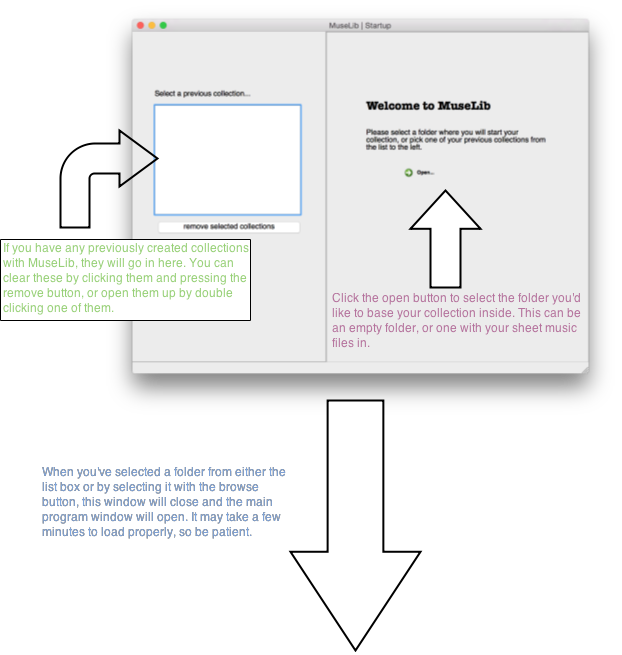
\includegraphics[width=400pt]{startup}
\caption{The window which will display on startup}
\label{fig:startup}	
\end{figure}

\subsection{Main view}
After the program has loaded, the main window shown in figure \ref{fig:main} will display. Panels to the left of this pane show a full listing of the files in your collection, which can be sorted by title, composer or lyricist, followed by a pane which displays any playlists you have created, followed by a third pane displaying playlists the system has generated for you. The auto generated playlists will automatically update with new pieces when you press the "refresh collection" option, located in the file menu.
\begin{figure}[H]
\centering
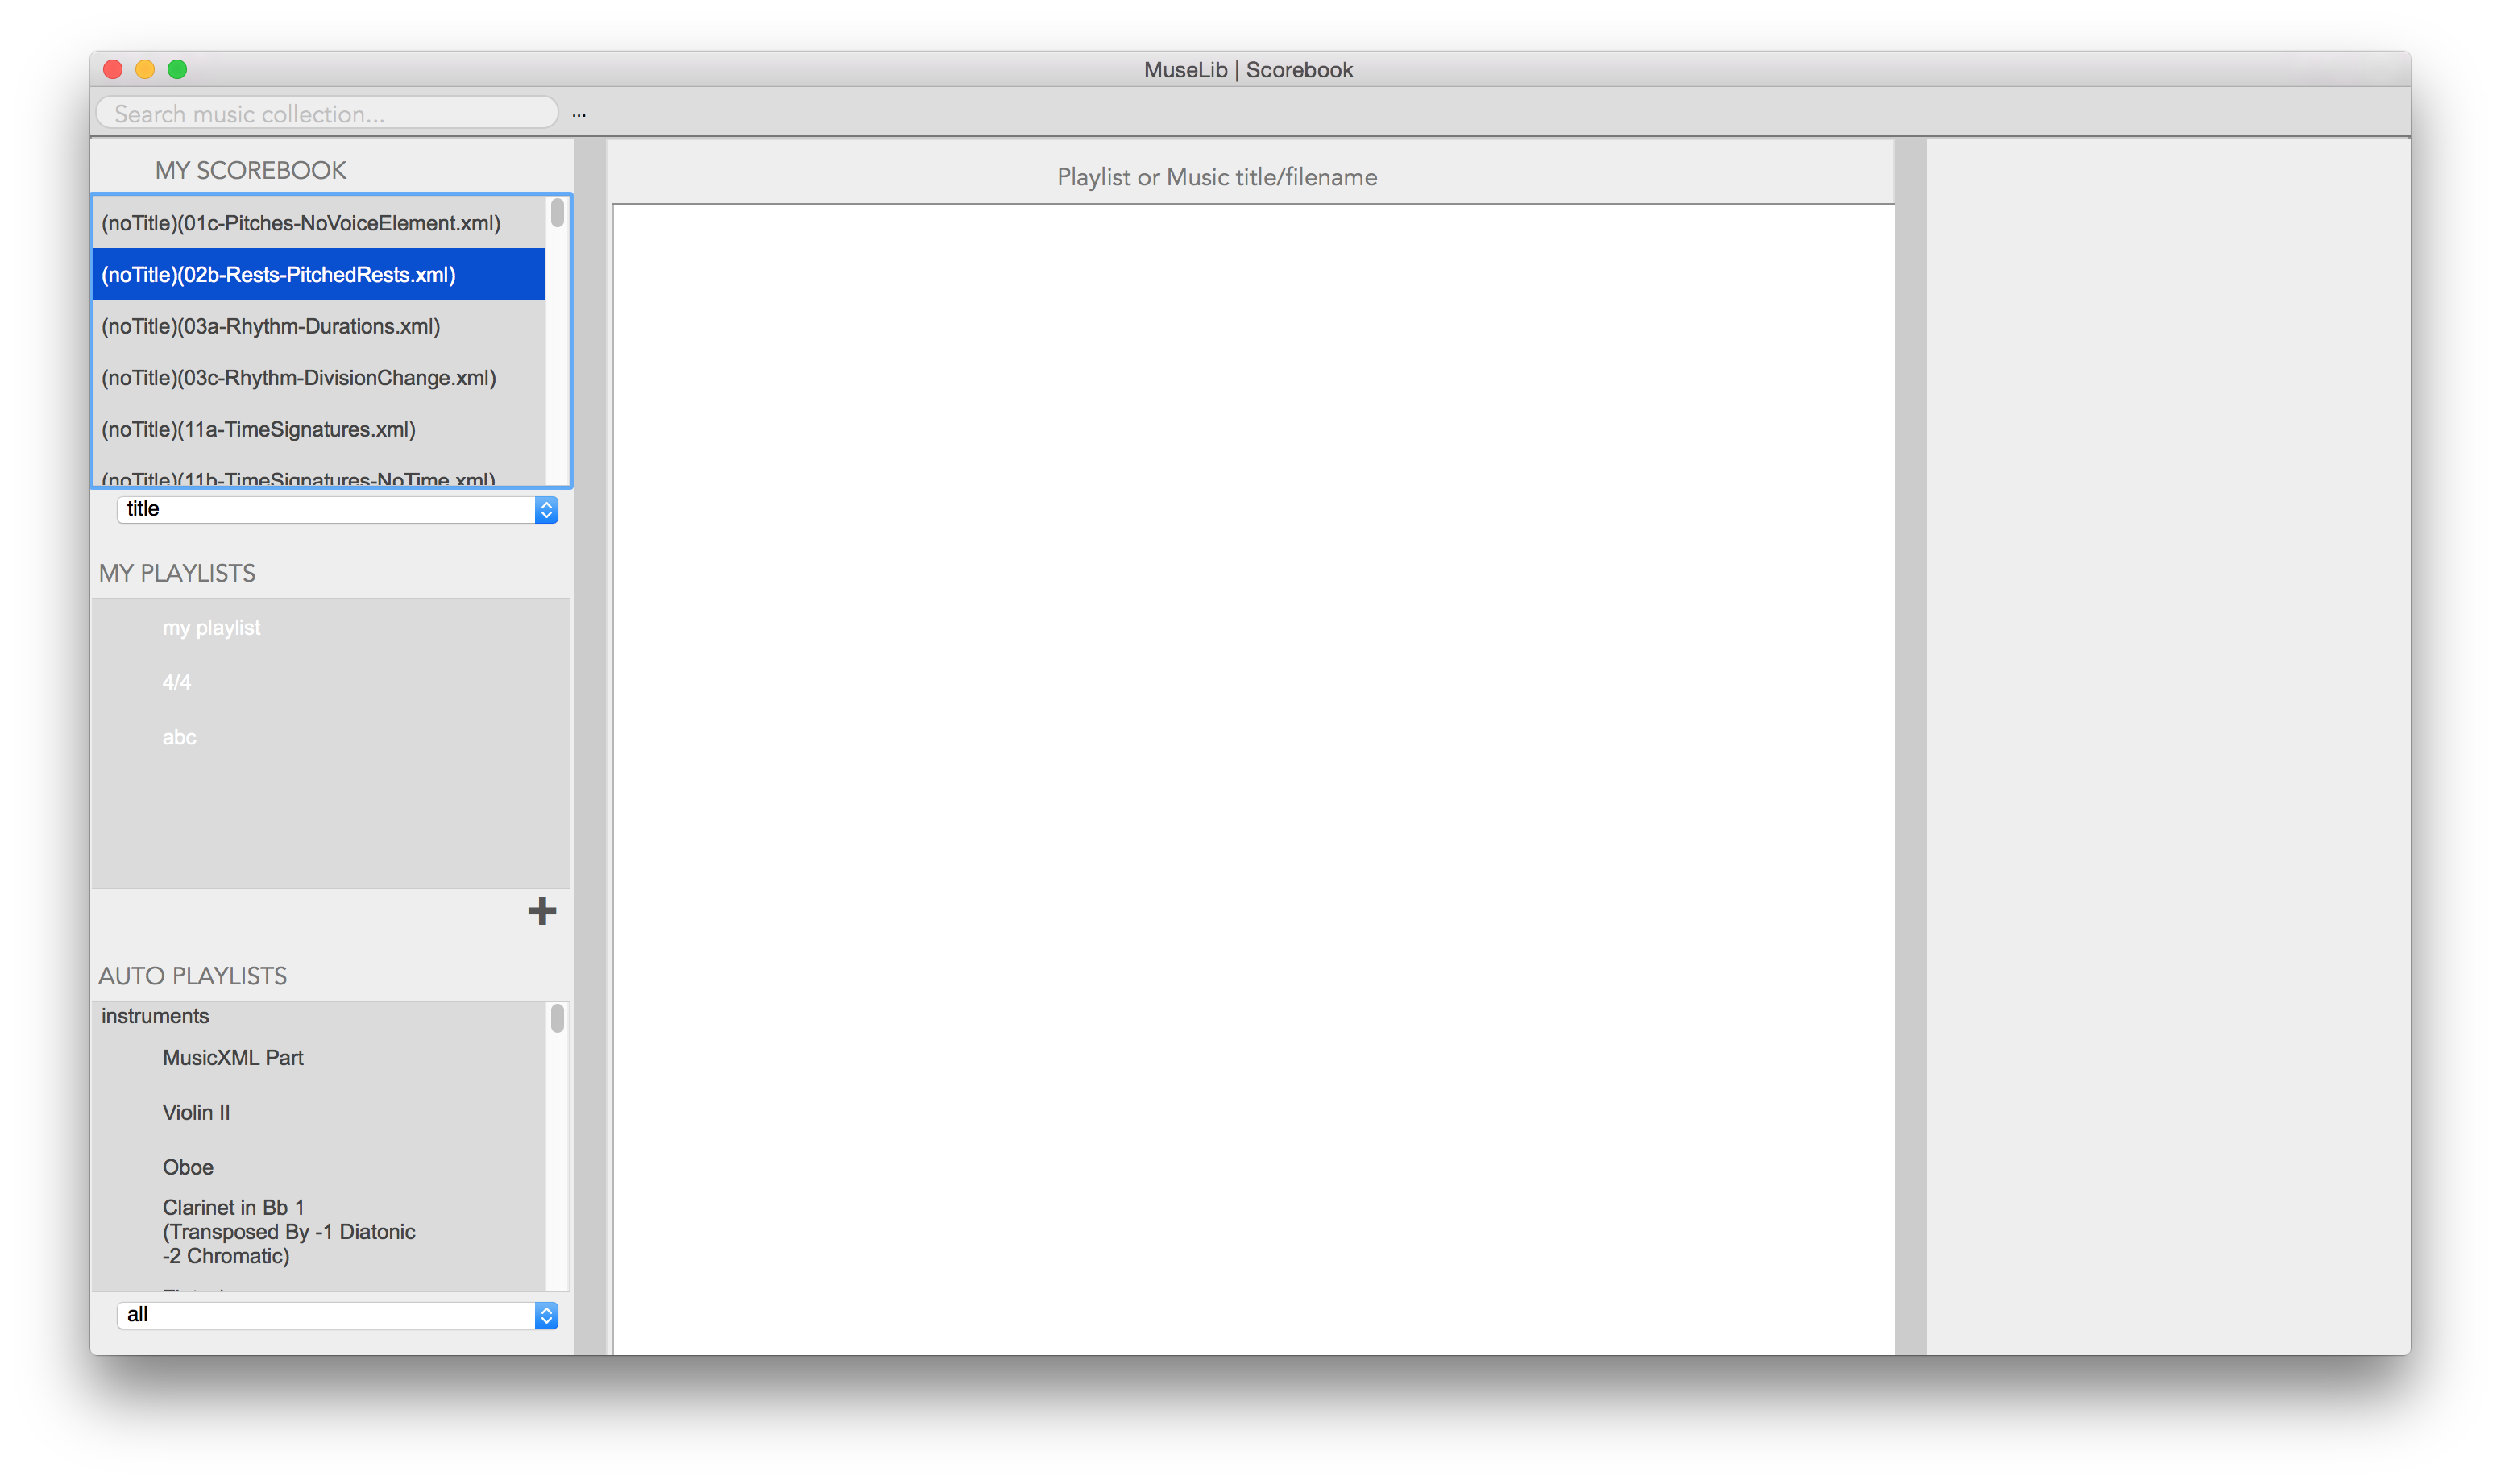
\includegraphics[width=500pt]{main_screenshot}
\caption{The window which will display on startup}
\label{fig:main}	
\end{figure}
\subsubsection{The User Created Playlist Widget}
The second widget from the top on the left is called the user created playlist widget. This will display all of the playlists you have created, as shown in figure \ref{fig:createdplaylists}. 
\begin{figure}[H]
\centering
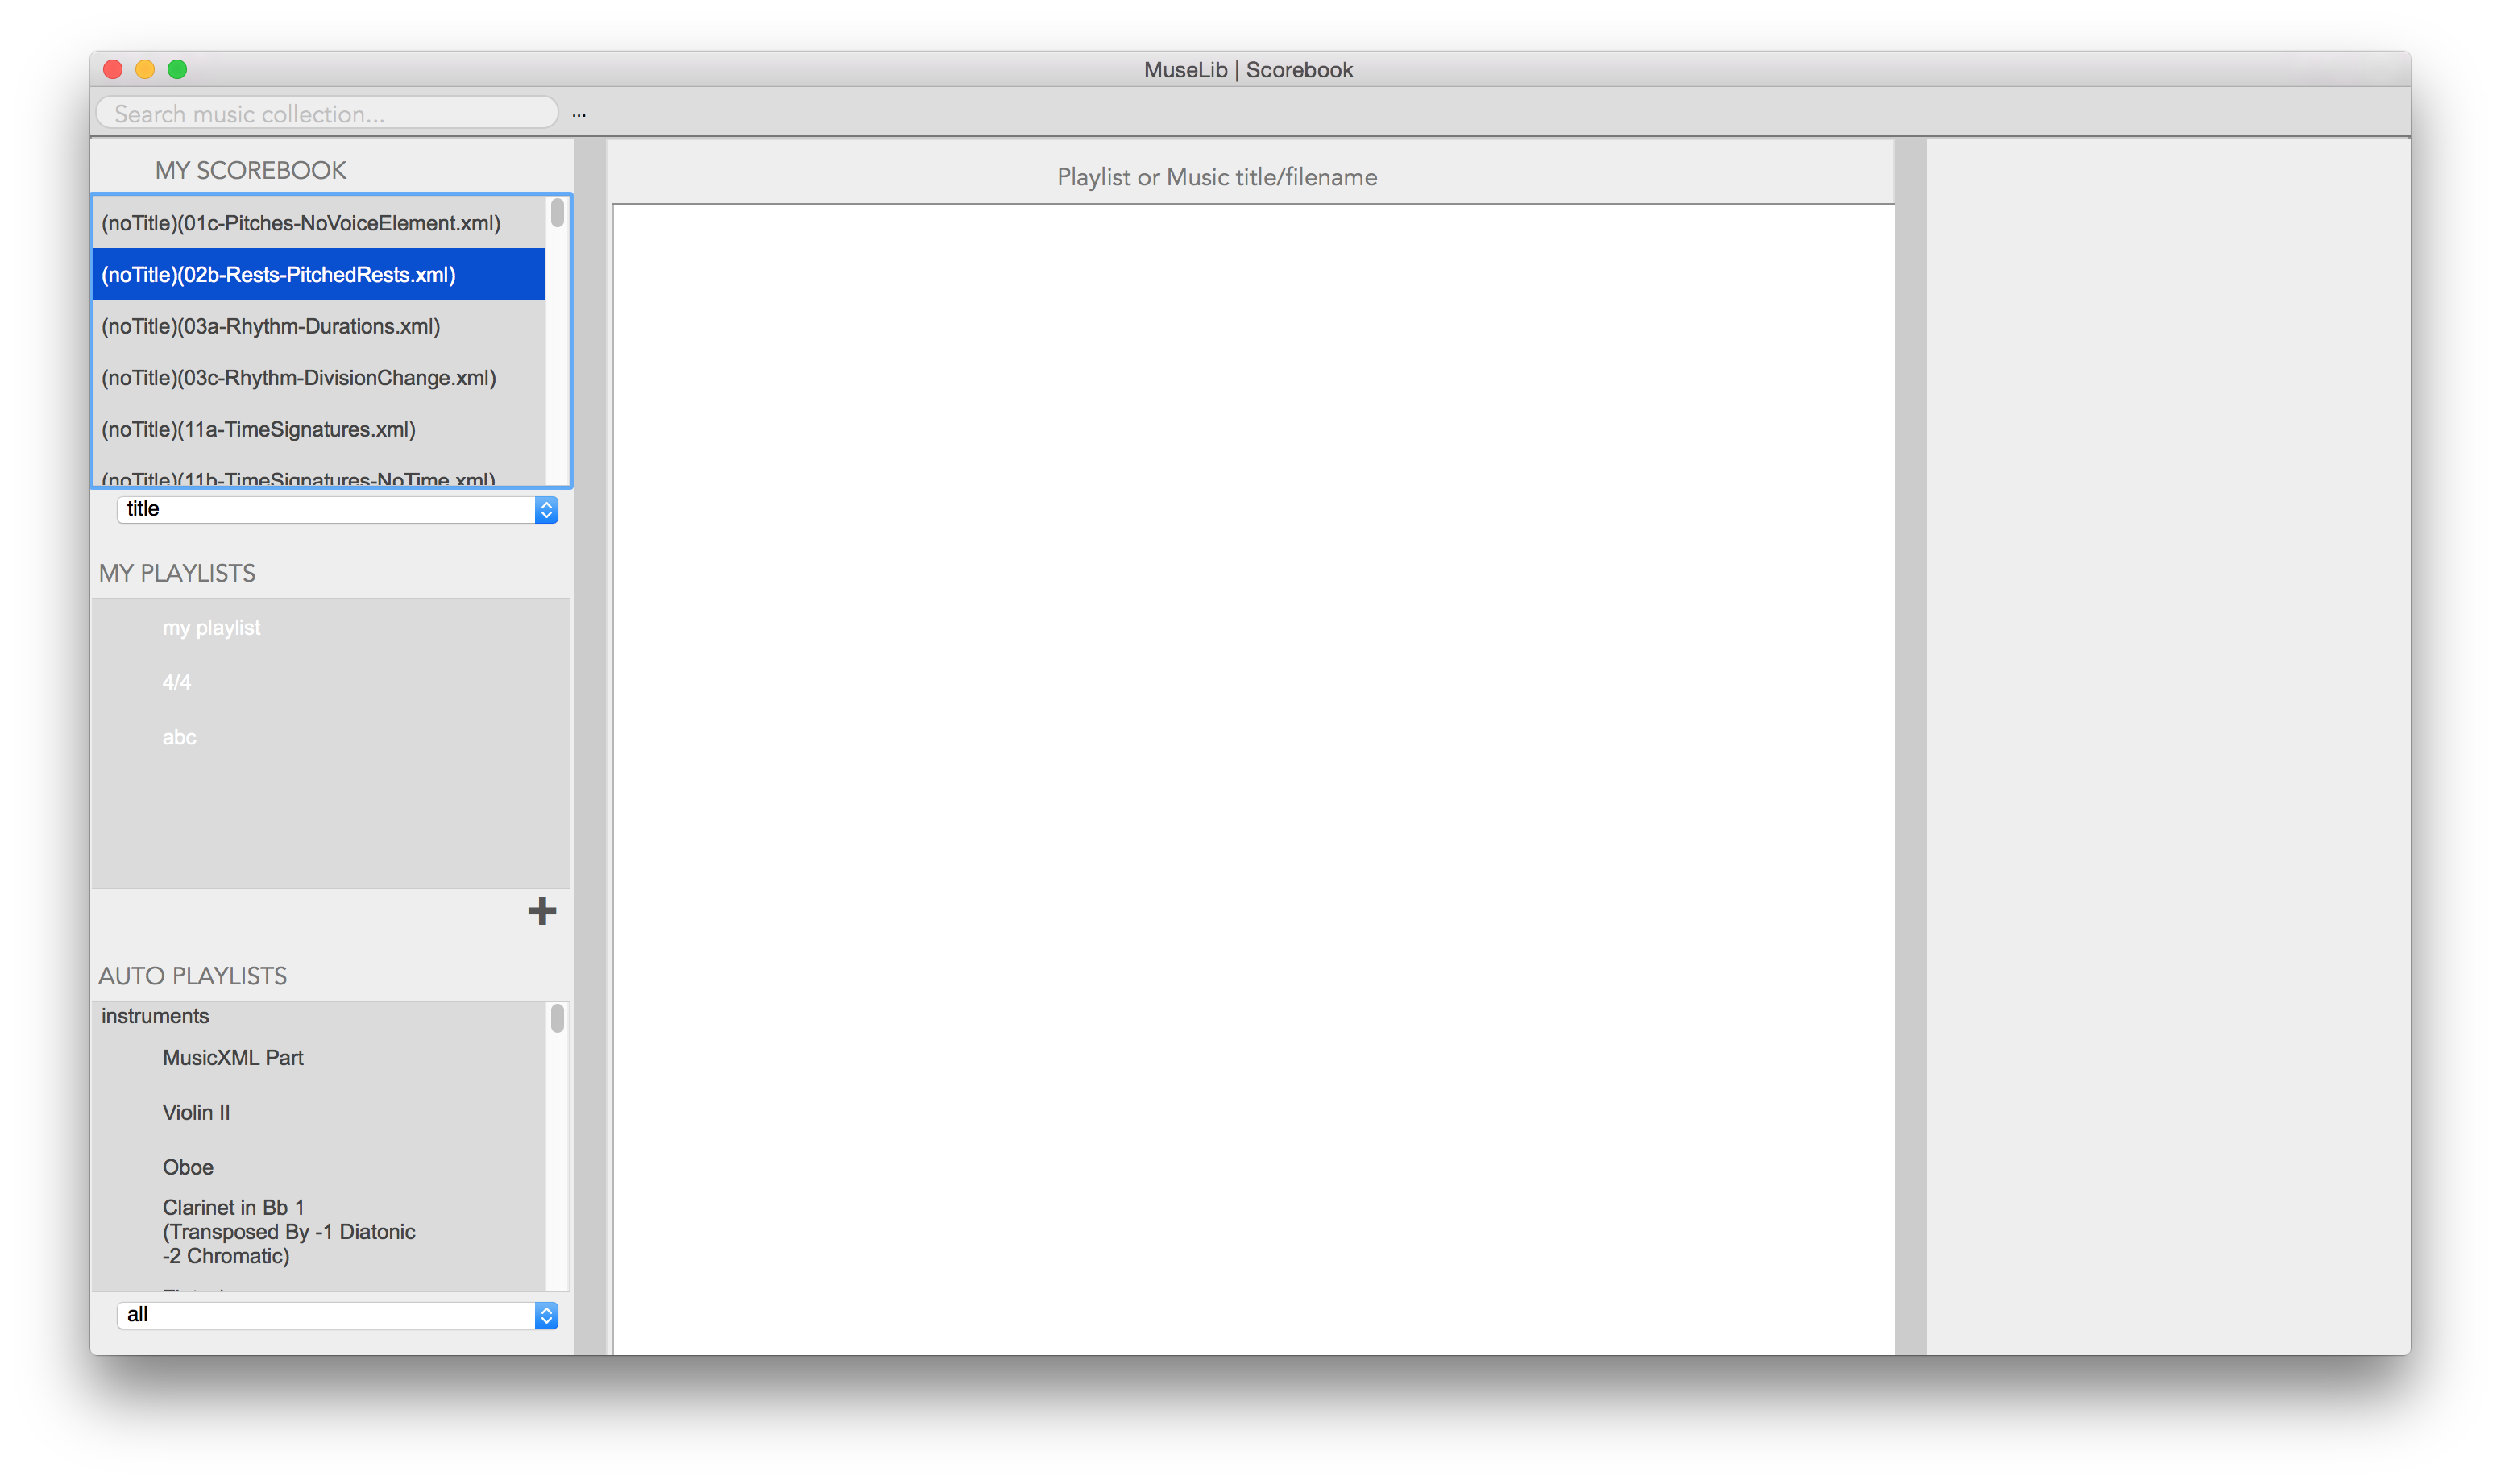
\includegraphics[width=500pt]{main_screenshot}
\caption{Window with playlists created by a user listed in second widget}
\label{fig:createdplaylists}	
\end{figure}

To add a new playlist to this list, press the add button, and a new popup will display as shown in figure \ref{fig:newplaylist}. Enter a title for this playlist, and search for pieces. The search functionality of this window is the same as the main window, as explained in section 2.3, so enter any information about the piece such as time signature, key etc in the same way you would in the main search box. These will be listed in the listbox below the text entry box, and can be reordered by dragging. Pieces can be removed from this list by selecting the item and pressing delete.
\begin{figure}[H]
\centering
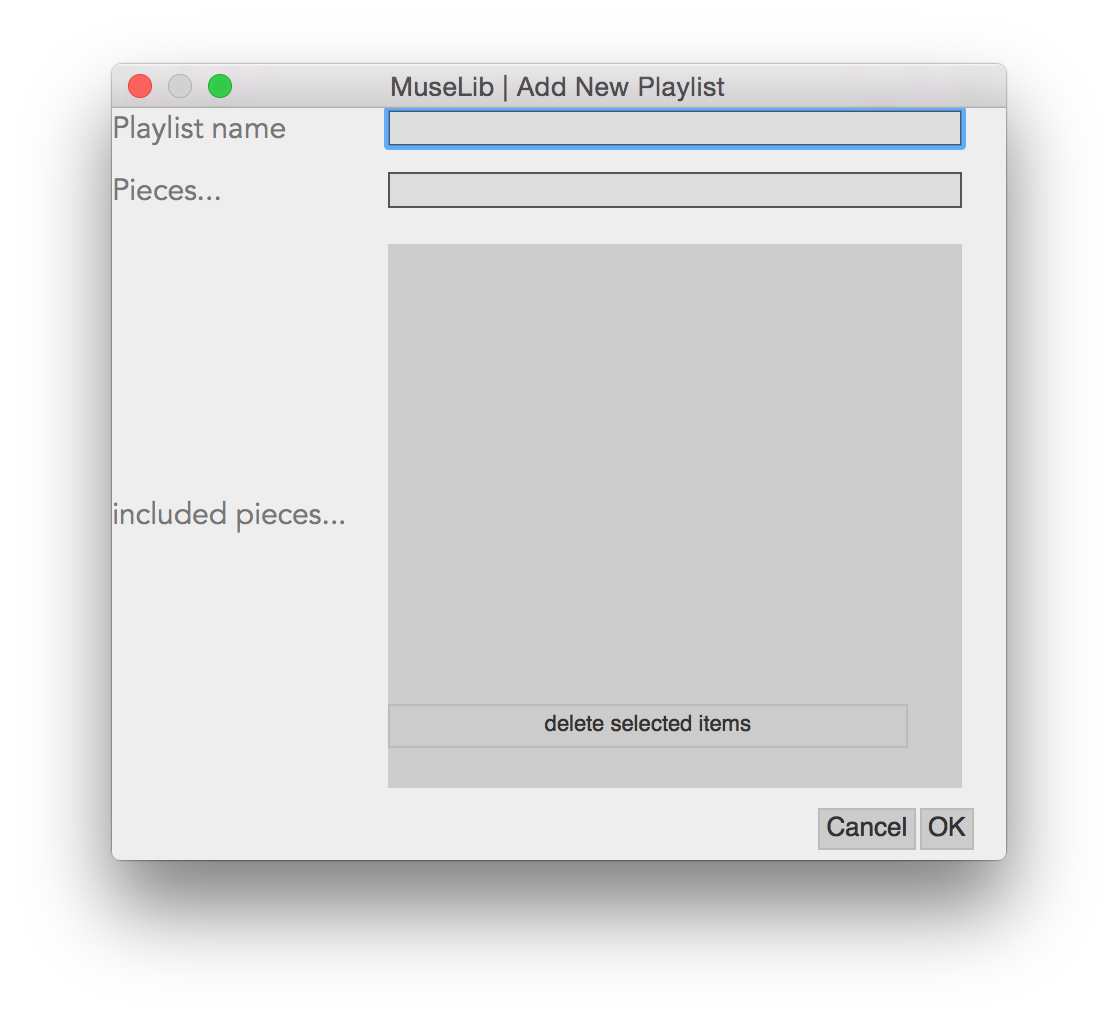
\includegraphics[width=\textwidth]{playlistpop}
\caption{Popup window for creating new playlists}
\label{fig:newplaylist}	
\end{figure}
Finally, press OK and the playlist will display in the widget to the left.

\subsection{Searching}
The search box at the top of the application allows you to browse your collection by entering information about the piece, as shown in figure \ref{fig:search}.
\begin{figure}[H]
\centering
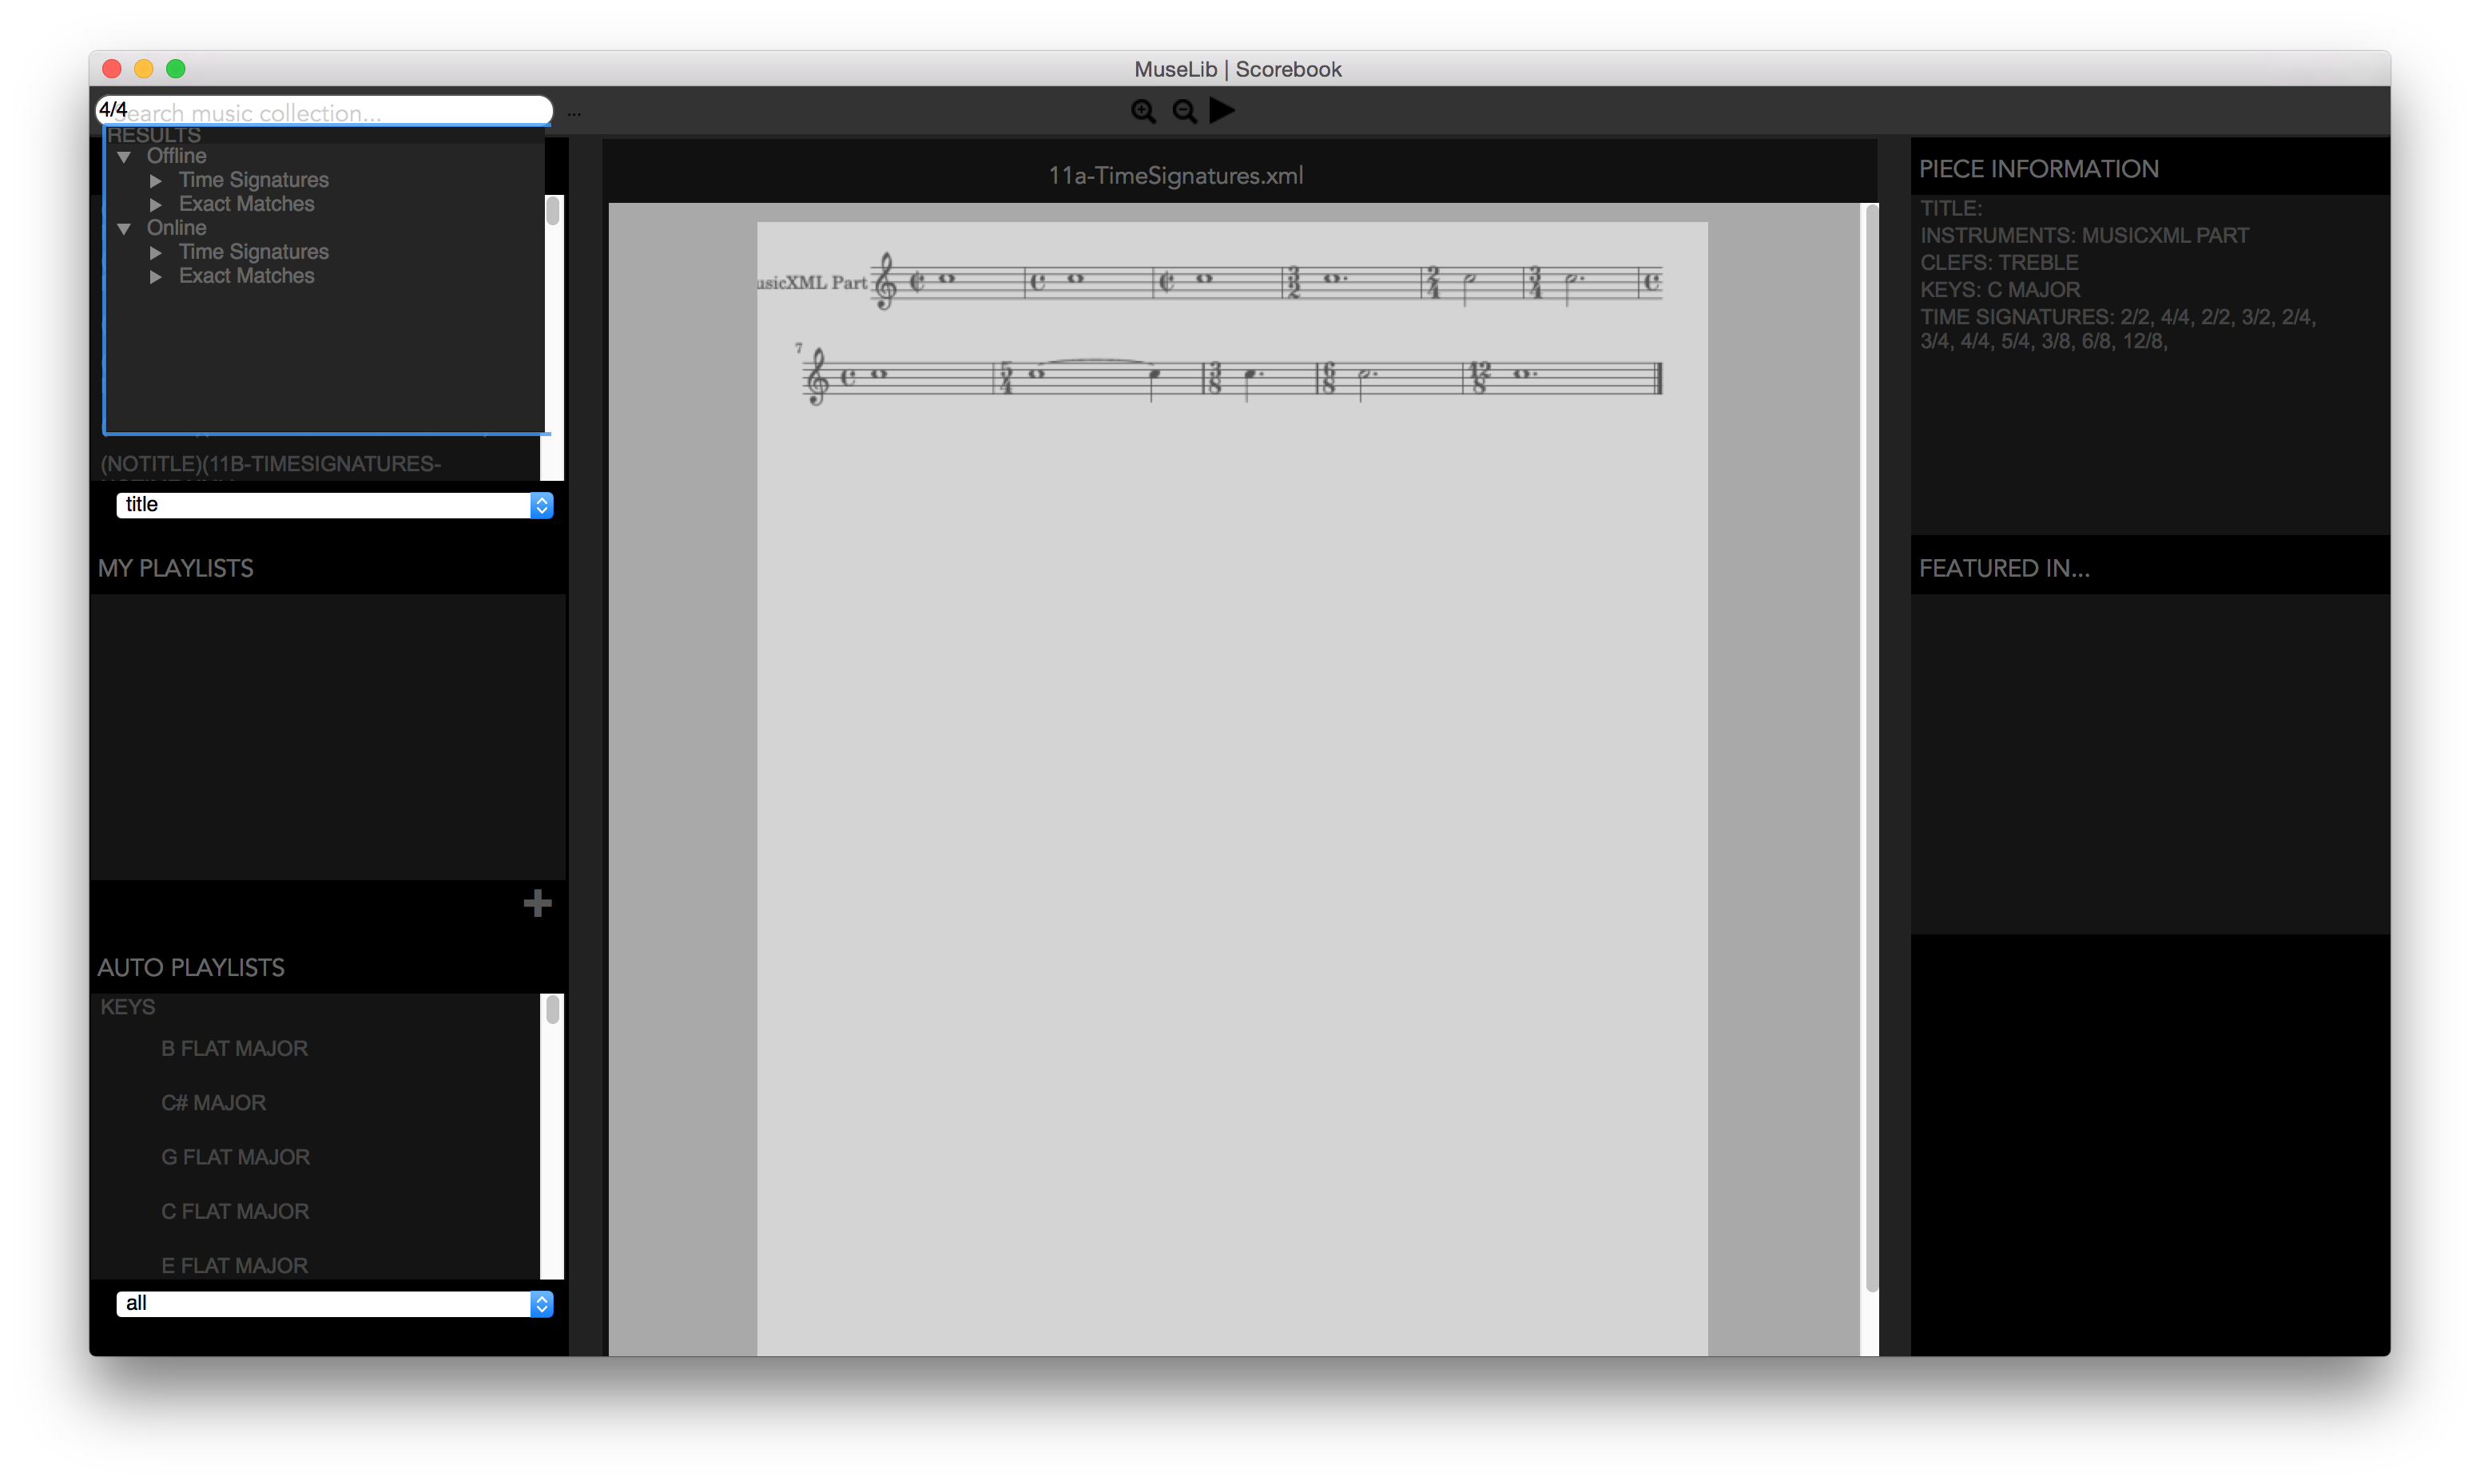
\includegraphics[width=500pt]{main_results}
\caption{Main window with search input results displaying}
\label{fig:search}	
\end{figure}

\subsubsection{Simple Searches}
In some instances, such as the query above, you may enter text into the box without needing to tell the system what you are looking for. Table \ref{table:commands} shows some of the commands you can use, separated by spaces.

\begin{table}[H]
\begin{tabu} to 1.05\textwidth {| X[l] | X[c] |} \hline
{Command} & {Result} \\ \hline
$<$letter$><$space$>$ followed by Major or Minor & System will look for pieces in this key (ignoring transposing instruments) \\ \hline
$<$number$>$/$<$number$>$ & System will search for a time signature \\ \hline
$<$rhythmicname$>$=$<$value$>$ & System will search for a tempo, where rhythmic name means quarter/crotchet, half/minim etc. \\ \hline
Text abc def & System will search individually for any pieces where the file name, title, composer, instrument names or lyricist match any of the individual words \\ \hline
"My name is fred" & System will search for the exact quote in all of the above \\ \hline
\end{tabu}
\caption{A table describing the command options for simple searches}
\label{table:commands}
\end{table}

\subsubsection{Complex Searches}
The structure laid out in section 2.3.1 manages to predict the majority of searches you might want to enter. However, some queries require more complexity, and as such "labels" are provided in order to achieve this. These are given in table \ref{table:commands_complex}.
\begin{table}[H]
\begin{tabu} to 1.05\textwidth {| X[l] | X[l] |} \hline
{\textbf{Command}} & {\textbf{Result}} \\ \hline
key:"C major" & System will look for pieces in this key \\ \hline
clef:treble & System will look for pieces with this clef in any part \\ \hline
meter:4/4 & System will search for a time signature \\ \hline
instrument:clarinet with:key:"C major" & System will search for pieces containing the instrument "clarinet" which is in the key of C major at some point in the piece \\ \hline
instrument:clarinet with:clef:bass & System will search for pieces containing the clarinet where the clarinet has a bass clef somewhere in the piece \\ \hline
instrument:clarinet with:clef:bass;key:"C major" & System will search for pieces containing the clarinet where the clarinet has a bass clef somewhere in the piece and is in C major somewhere in the piece \\ \hline
transposition:clarinet with:clef:bass;key:"C major" & System will search for pieces containing the clarinet, or if there is no clarinet, any instrument which has the same transposition \\ \hline
\end{tabu}
\caption{A table describing the command options for complex searches}
\label{table:commands_complex}
\end{table}

\subsubsection{Downloading new files}
When you search for files, the system will also provide you with suggestions which are located in online collections. You may choose to add these files to your collection simply by double clicking. This will open up a popup box as shown in figure \ref{fig:license}, which shows the license terms for that particular piece. When you click OK, the system will download and display the file.
\begin{figure}[H]
\centering
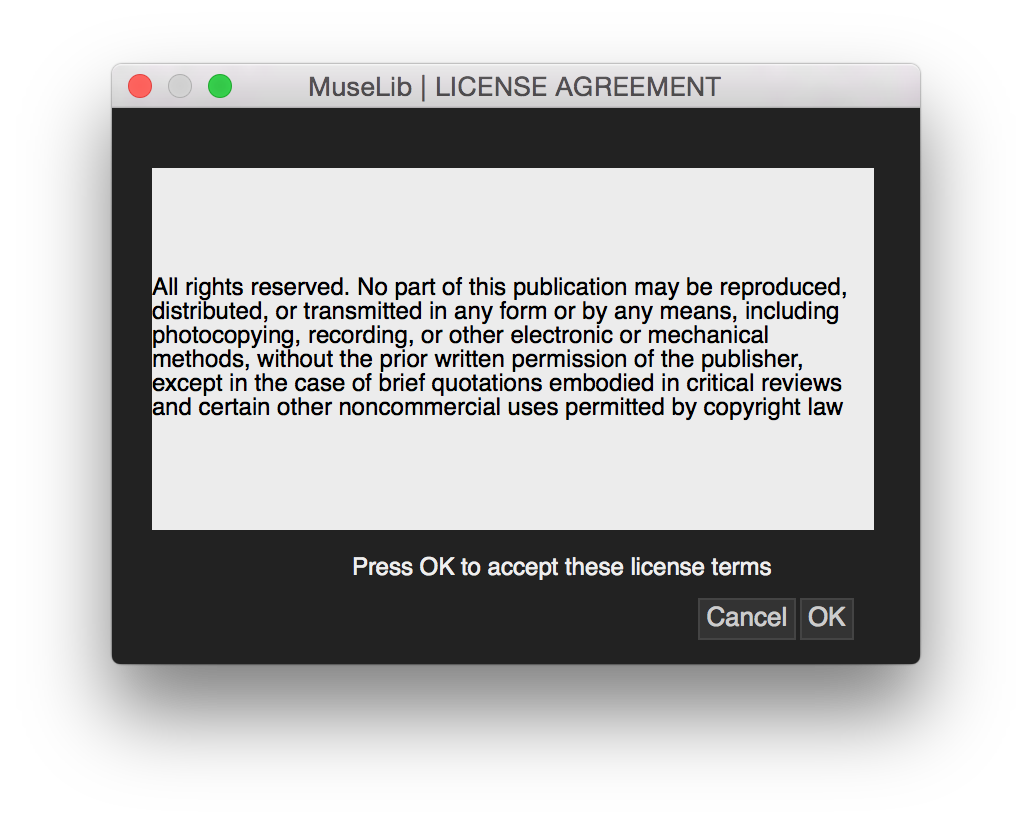
\includegraphics[width=400pt]{licensepop}
\caption{The popup which displays when a piece downloads}
\label{fig:license}	
\end{figure}

\subsection{Piece view}
When you view a piece, it will display in the middle portion and update the panes to the right according to data found, as shown in figure \ref{fig:piece}. The first pane to the right is for information about this piece. This displays all the information the system knows about the given piece.
The second pane displays any playlists you have created which feature this piece.
The third pane is a minimised version of the playlist browser. This will only display if you loaded this piece from the playlist view, as shown in figure \ref{fig:playlist}

\begin{figure}[H]
\centering
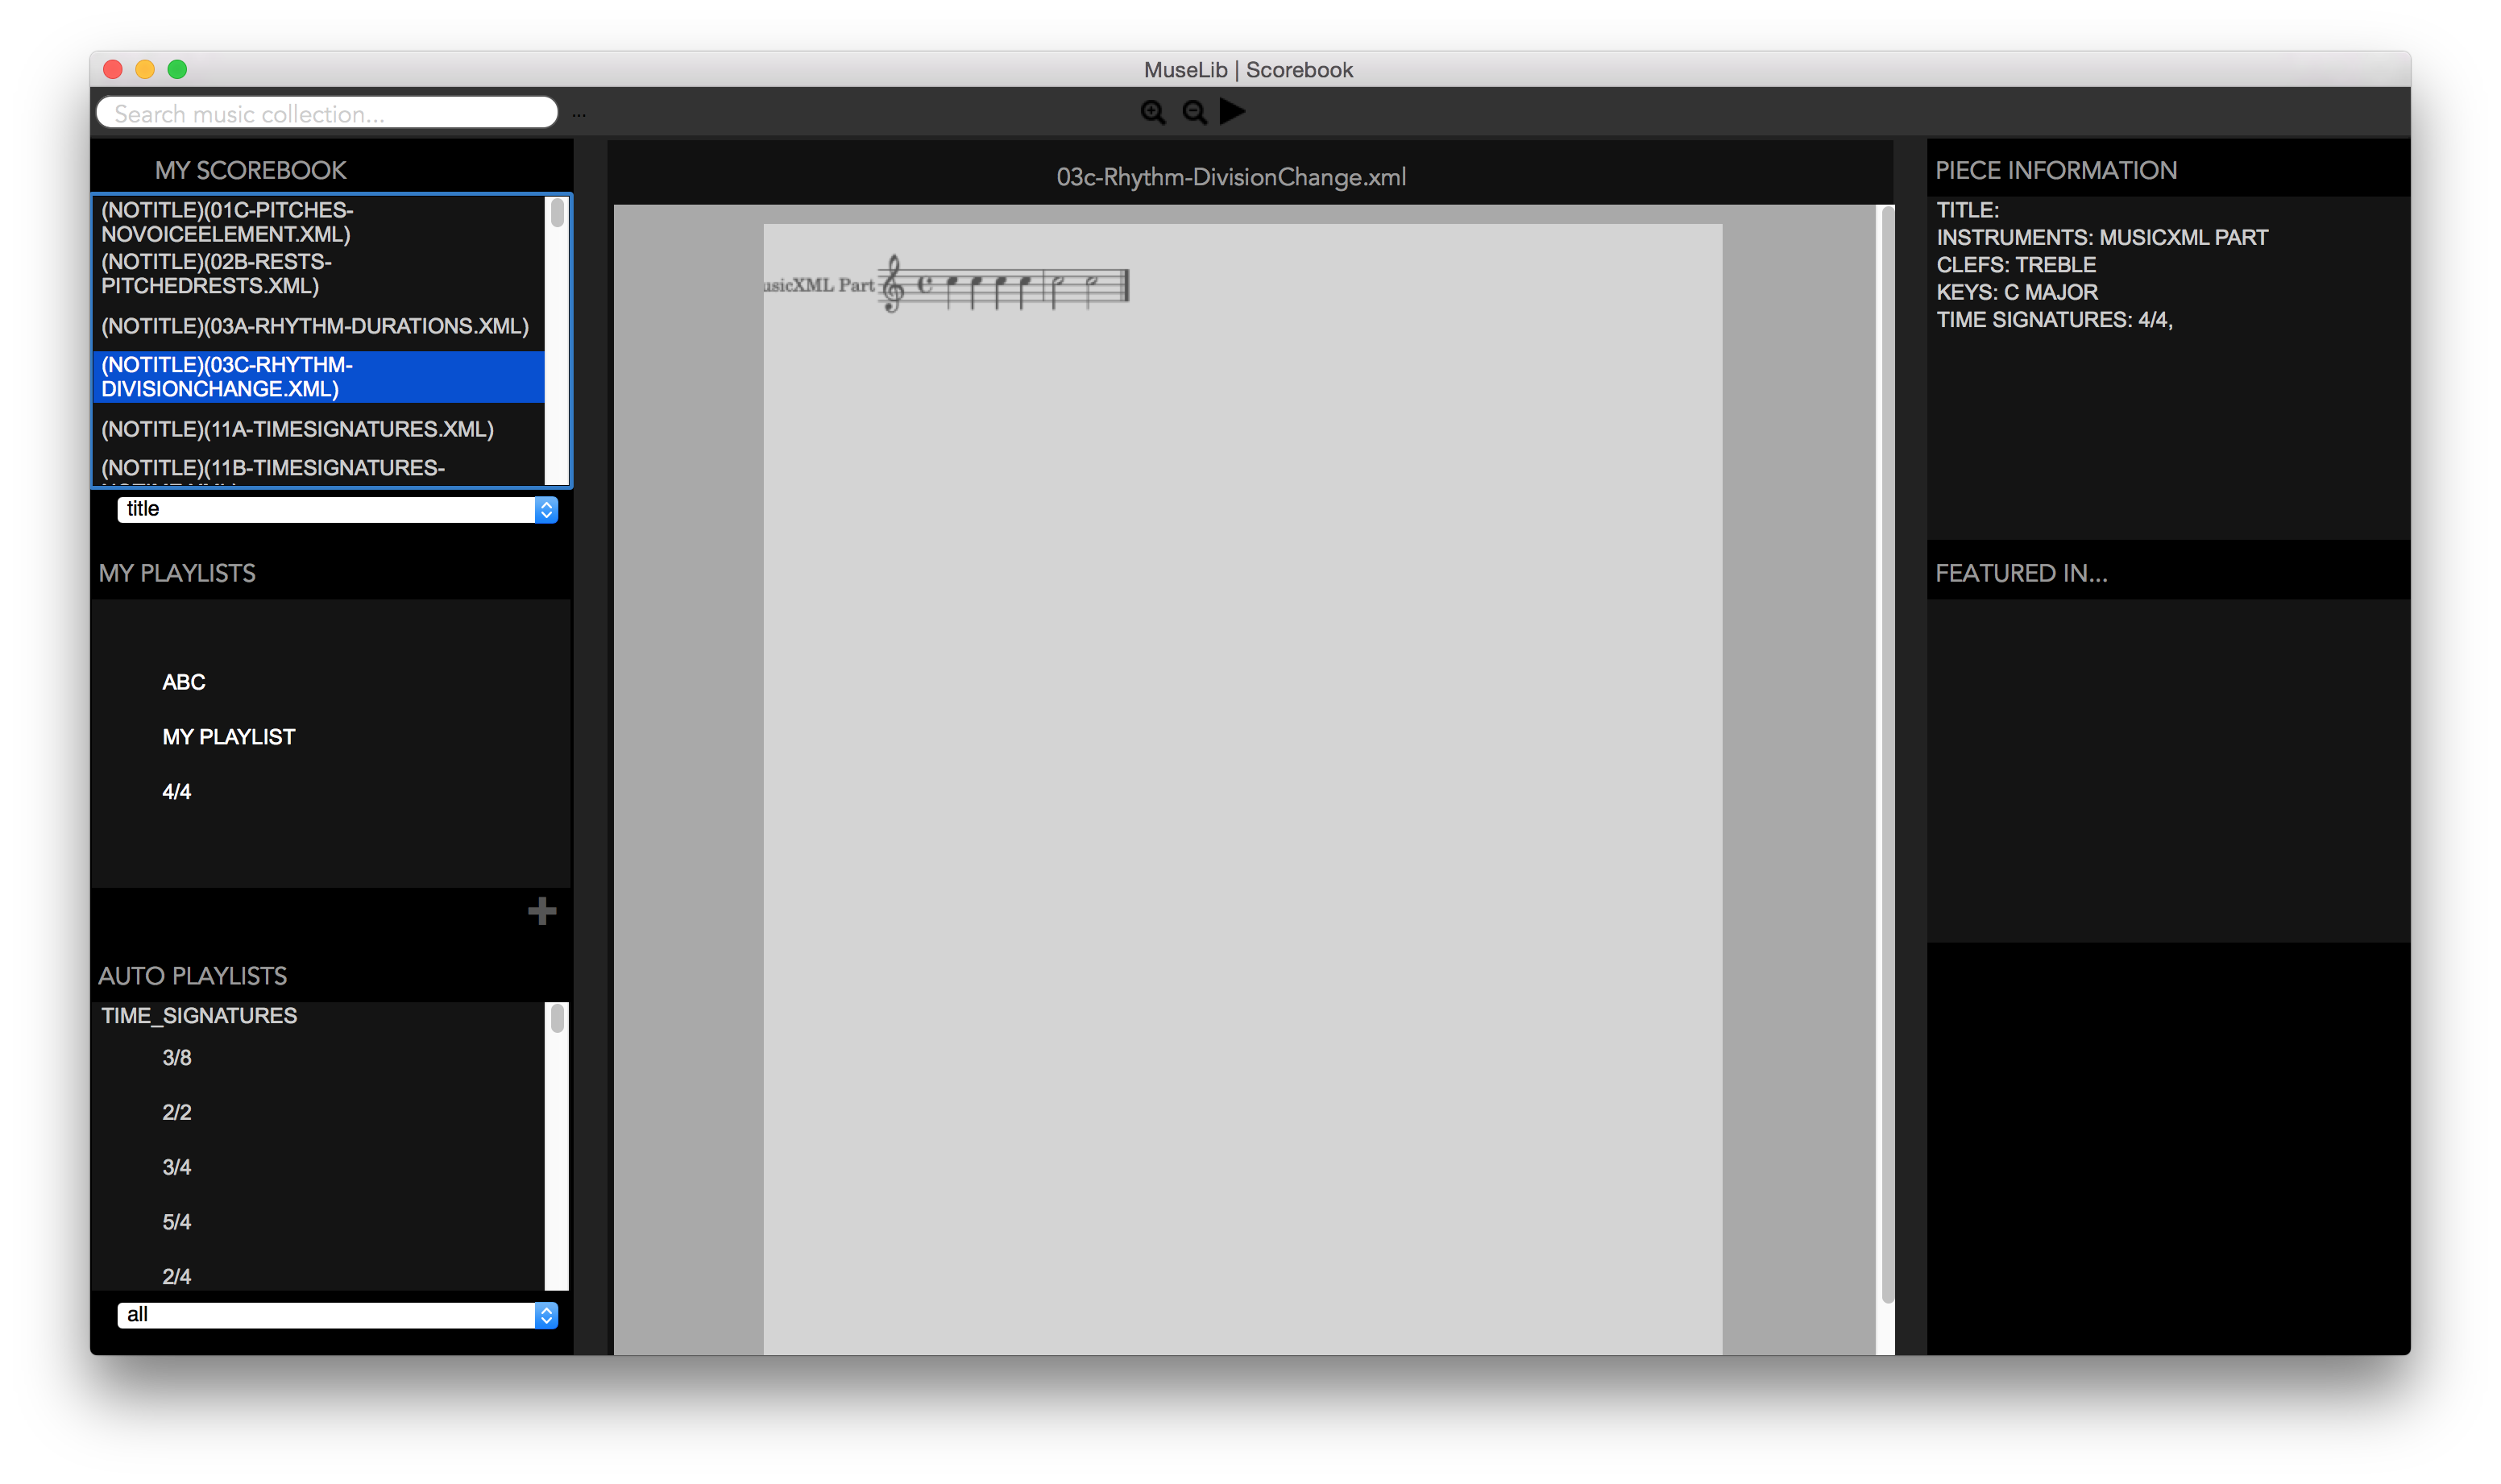
\includegraphics[width=500]{main_piece}
\caption{The main view showing a loaded piece}
\label{fig:piece}	
\end{figure}

There are also two buttons above the piece of music, the first of which allows you to zoom in, and the second zoom out. The third button is a feature which has yet to be put in.
\subsection{Playlist View}
When you select a playlist from either the user created widget or the auto generated playlists widget, the main window will update as shown in figure \ref{fig:playlist}. This displays a full list of pieces in the playlist together with all of the associated data.
\begin{figure}[H]
\centering
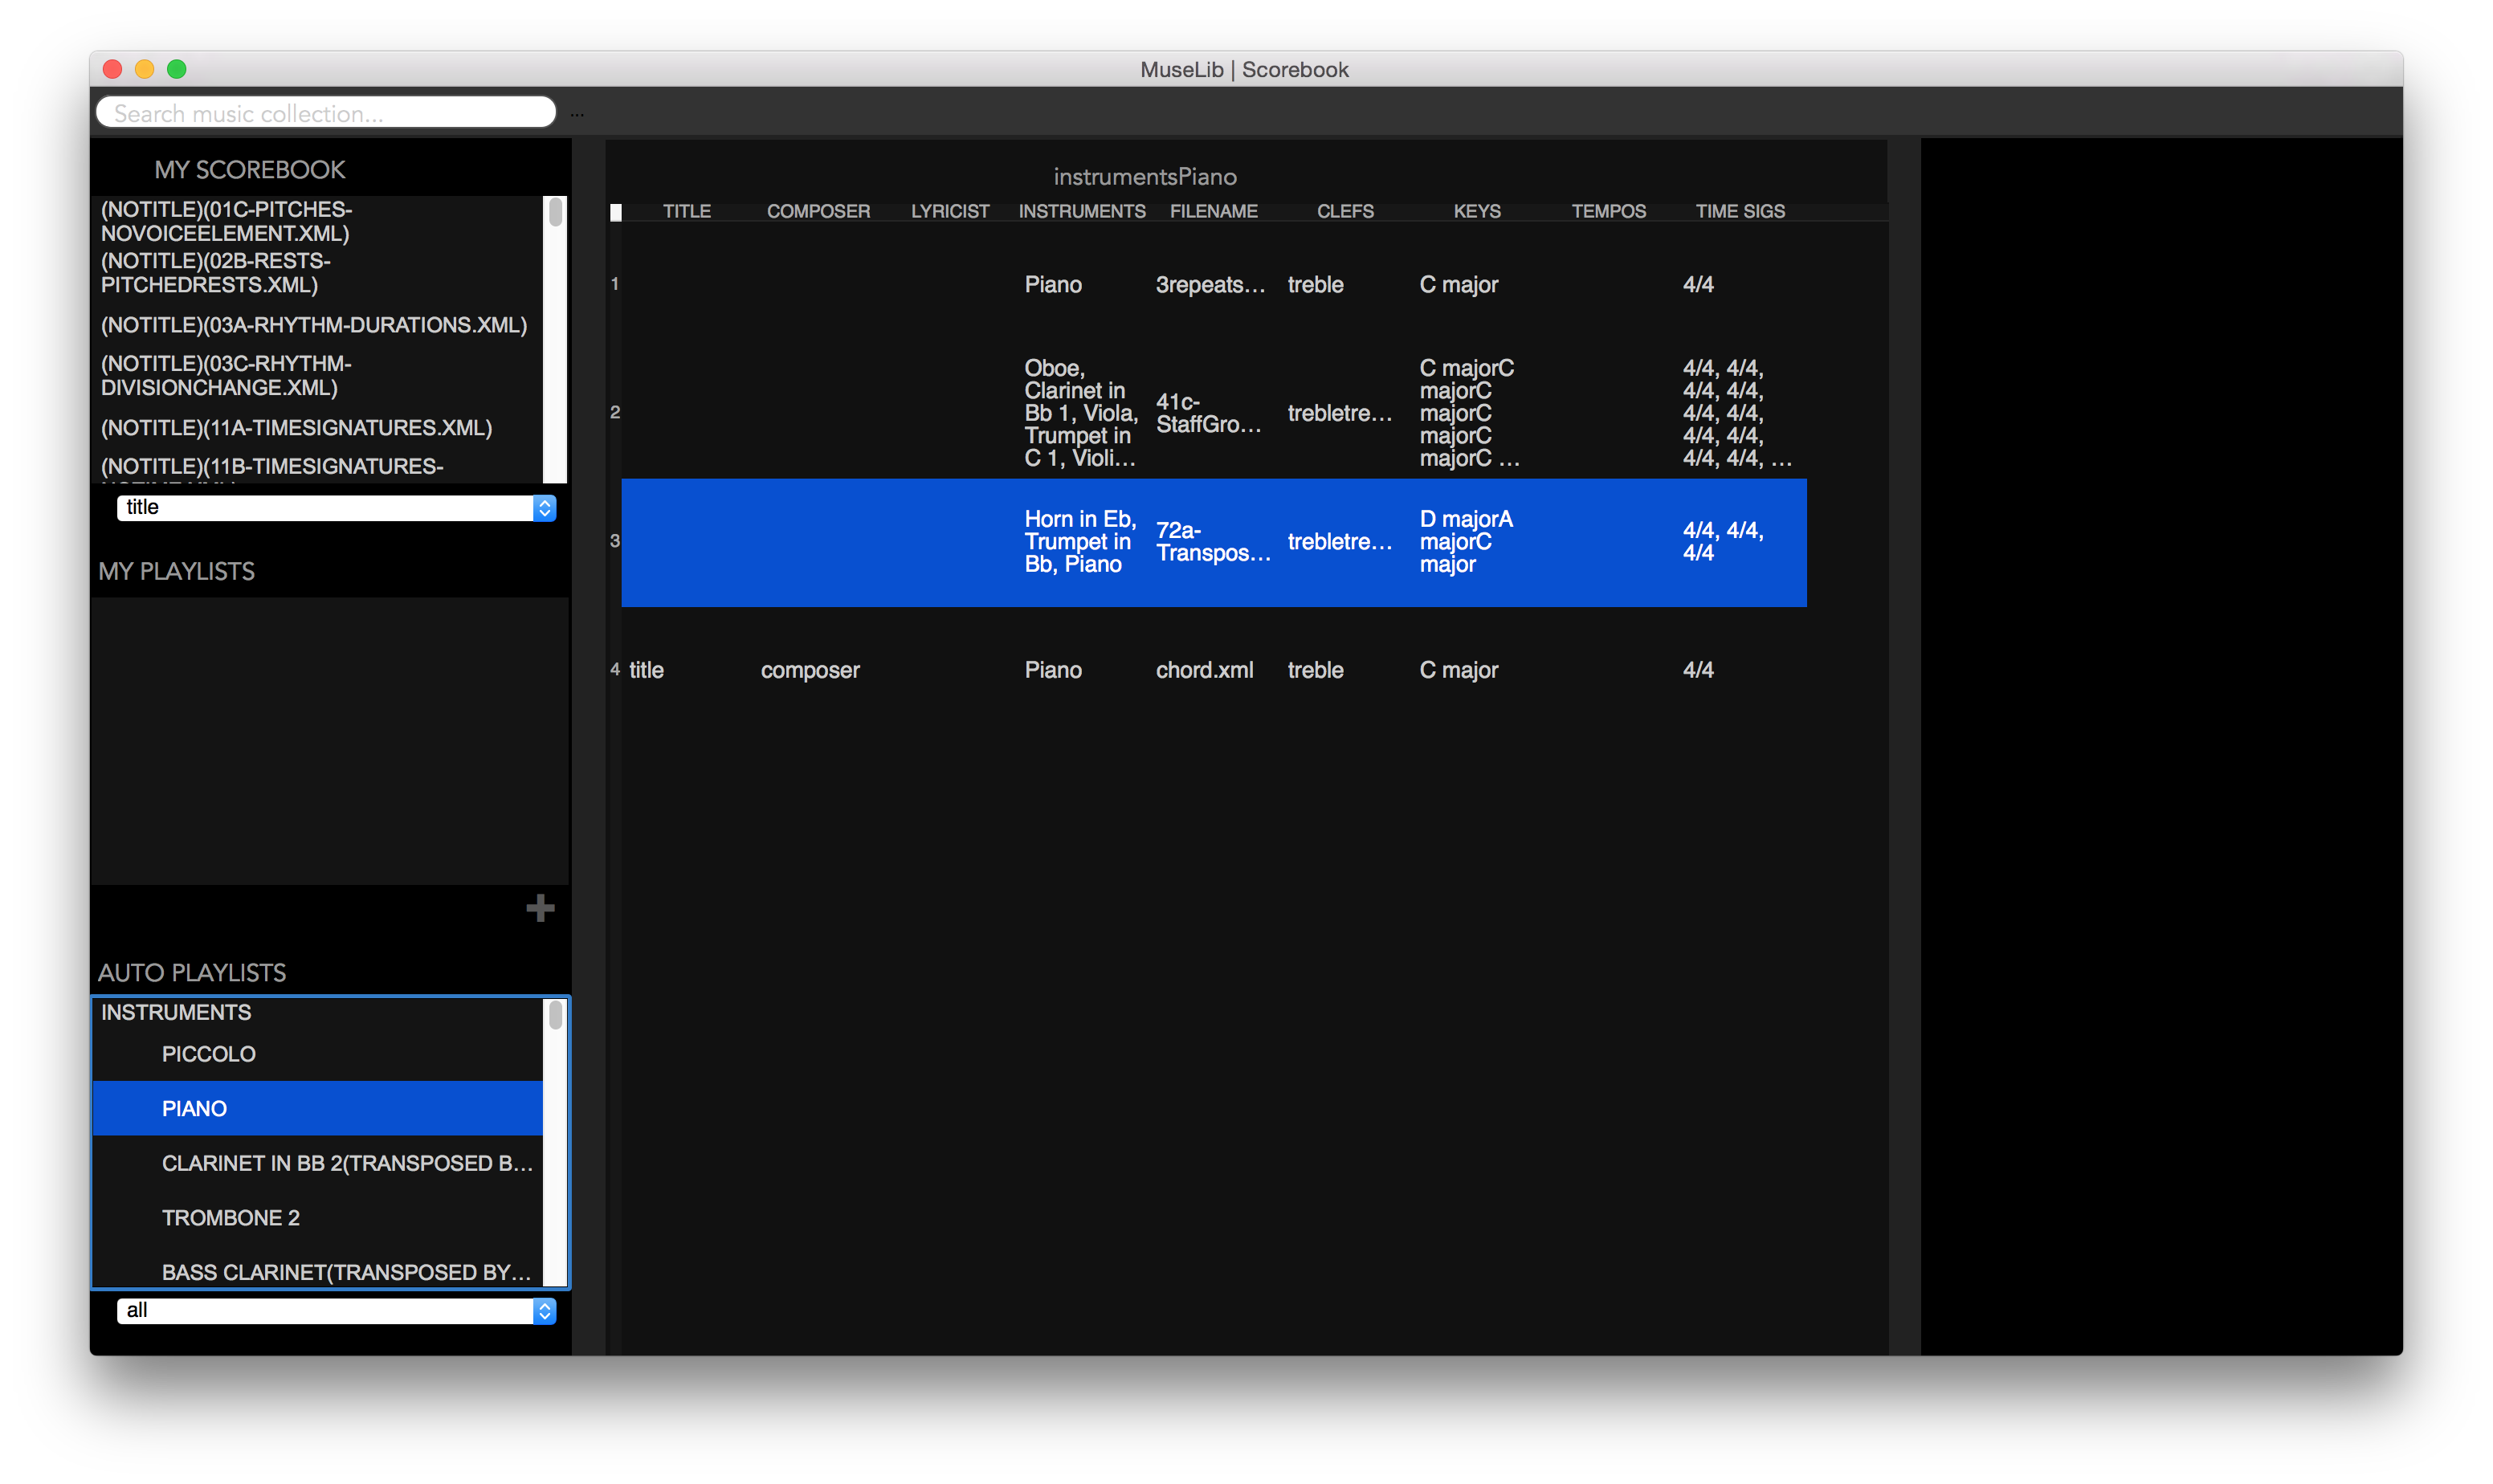
\includegraphics[width=500pt]{main_playlist}
\caption{The playlist view}
\label{fig:piece}	
\end{figure}

\subsubsection{Viewing a piece from the playlist view}
When you double click any of the pieces in a given playlist, the view will update as shown in figure \ref{fig:playlistbrowser}. A third widget has been displayed on the right, showing a full listing of the playlist. The widget has also highlighted the current piece you have selected.
\begin{figure}[H]
\centering
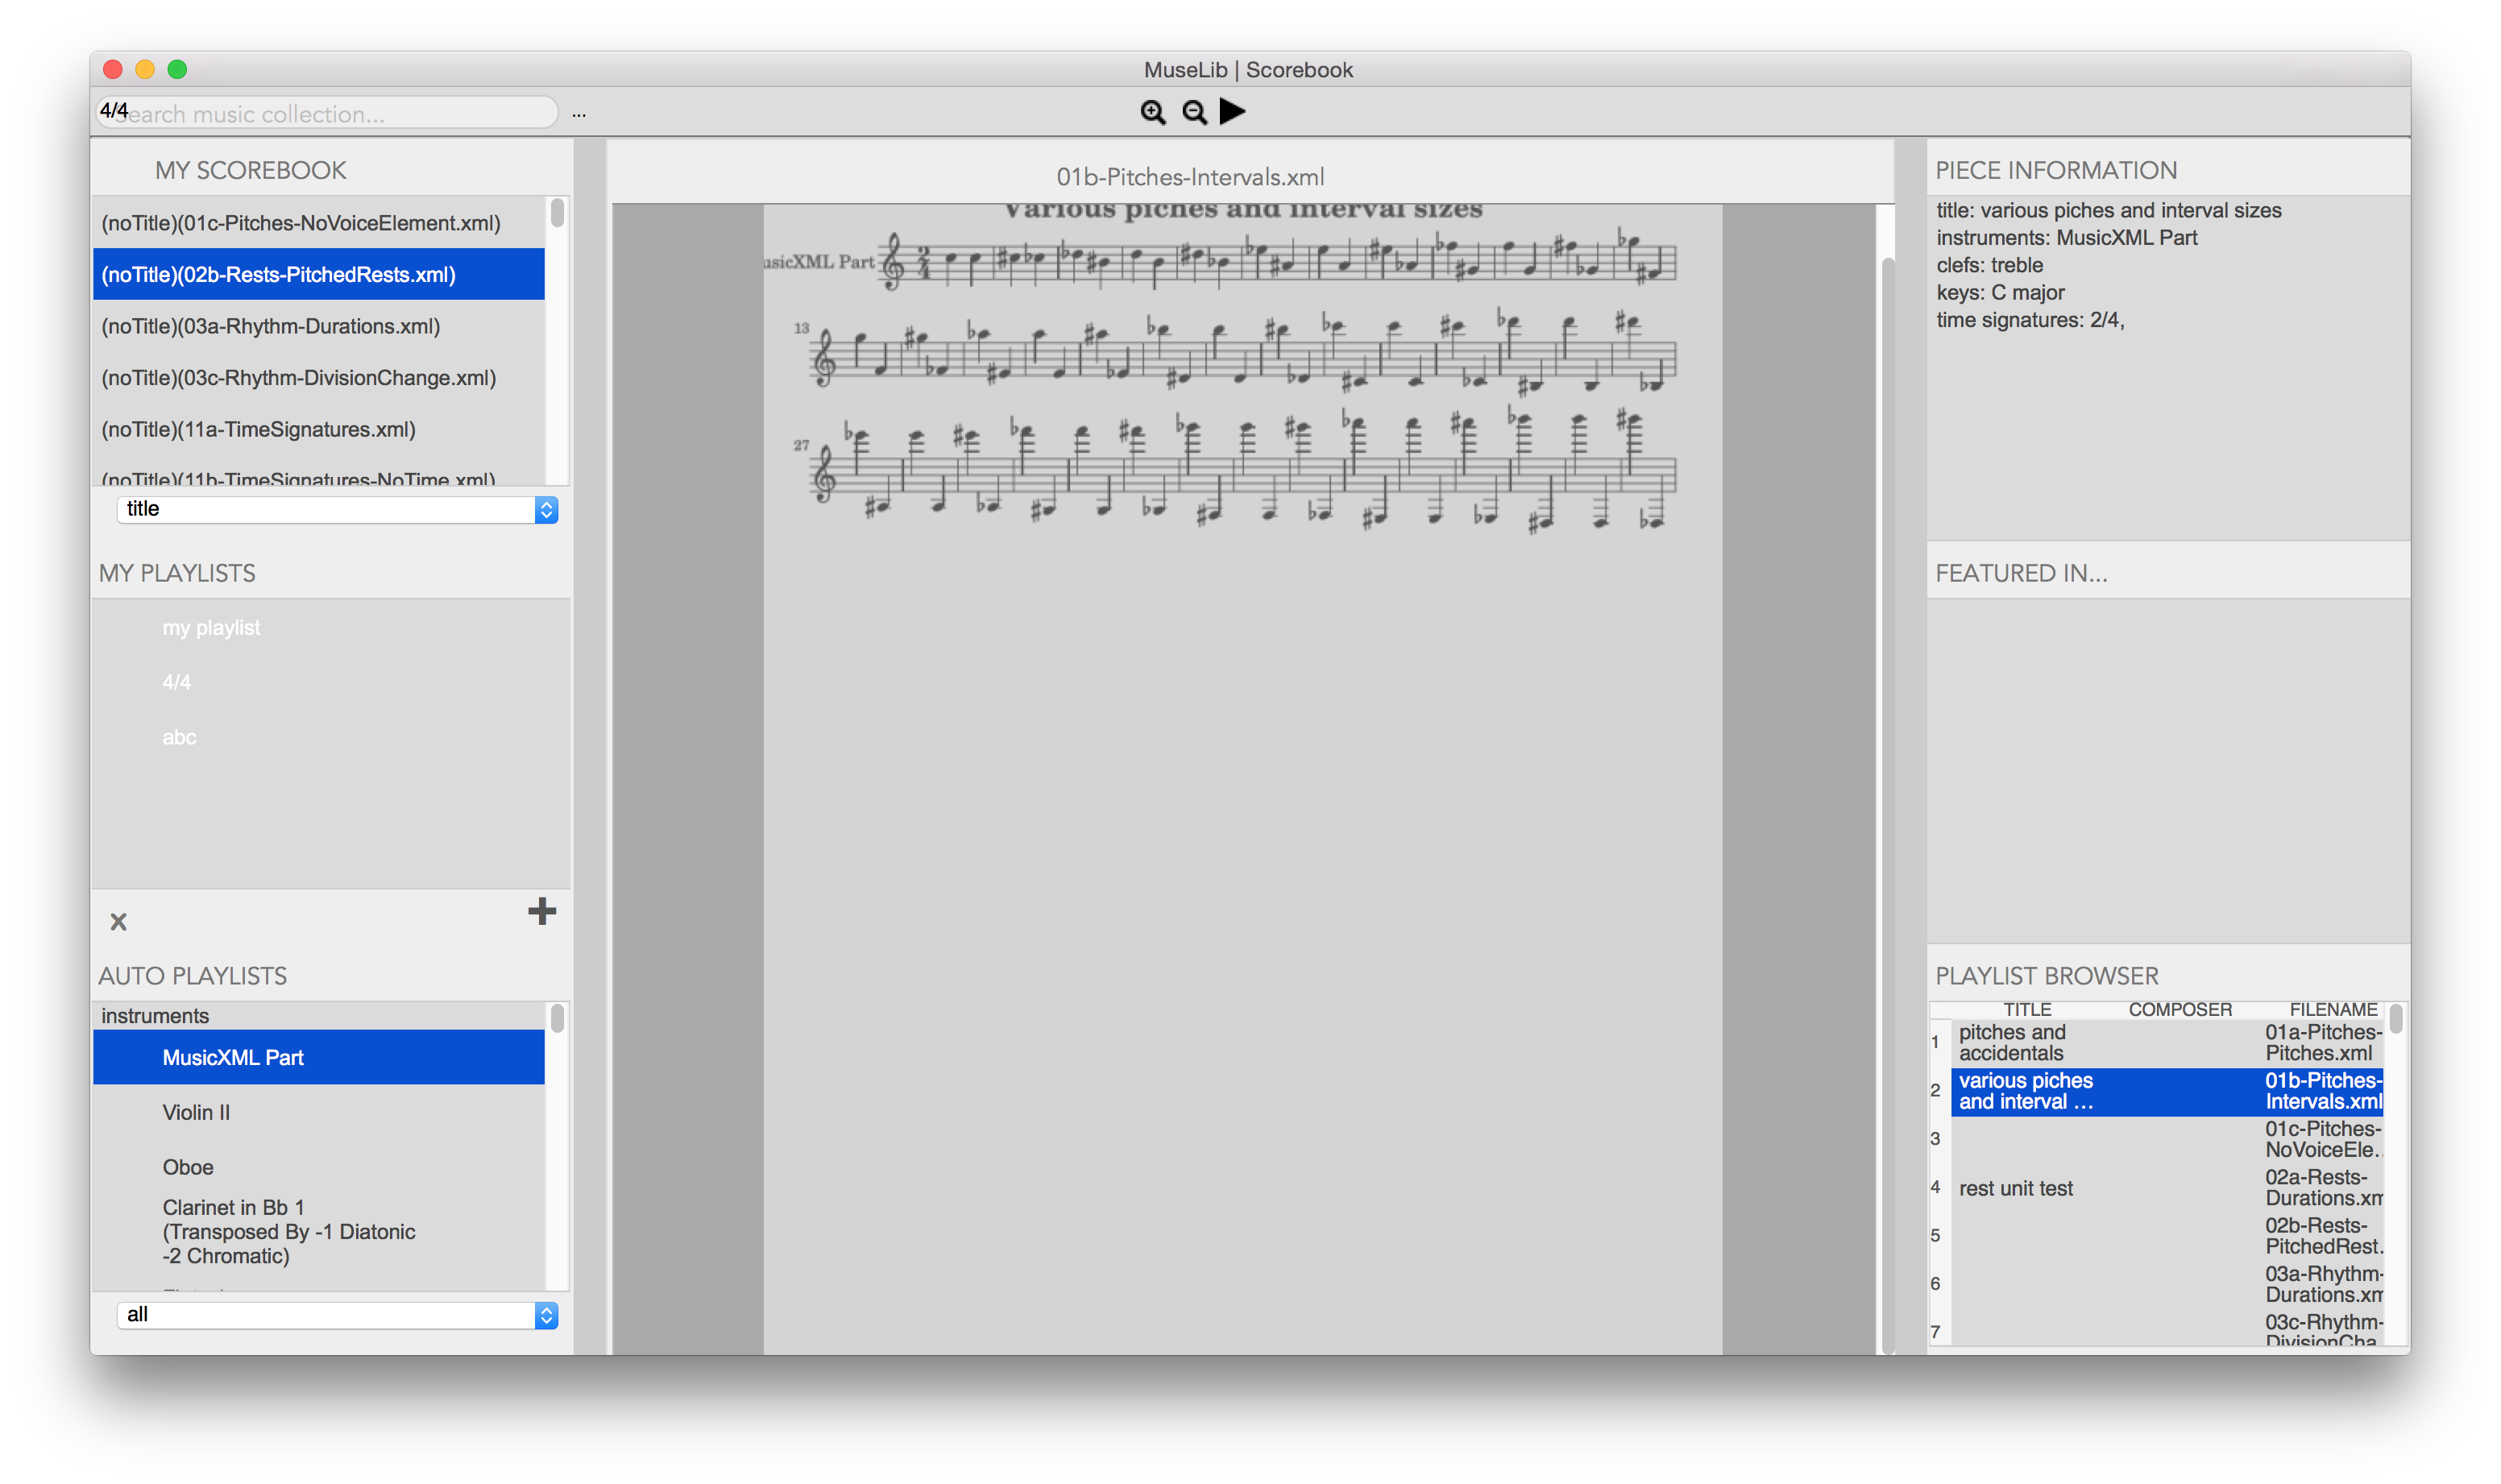
\includegraphics[width=500pt]{playlistbrowser}
\caption{The window which will display on startup}
\label{fig:playlistbrowser}	
\end{figure}

\subsection{Popups and Error Windows}
\subsubsection{The Import Popup}
If you wish to add a new file from inside the application which does not reside in the main collection folder, you may import it using the import window. To open it go to File->Import from the main window. The popup in figure \ref{fig:import} will display.
\begin{figure}[H]
\centering
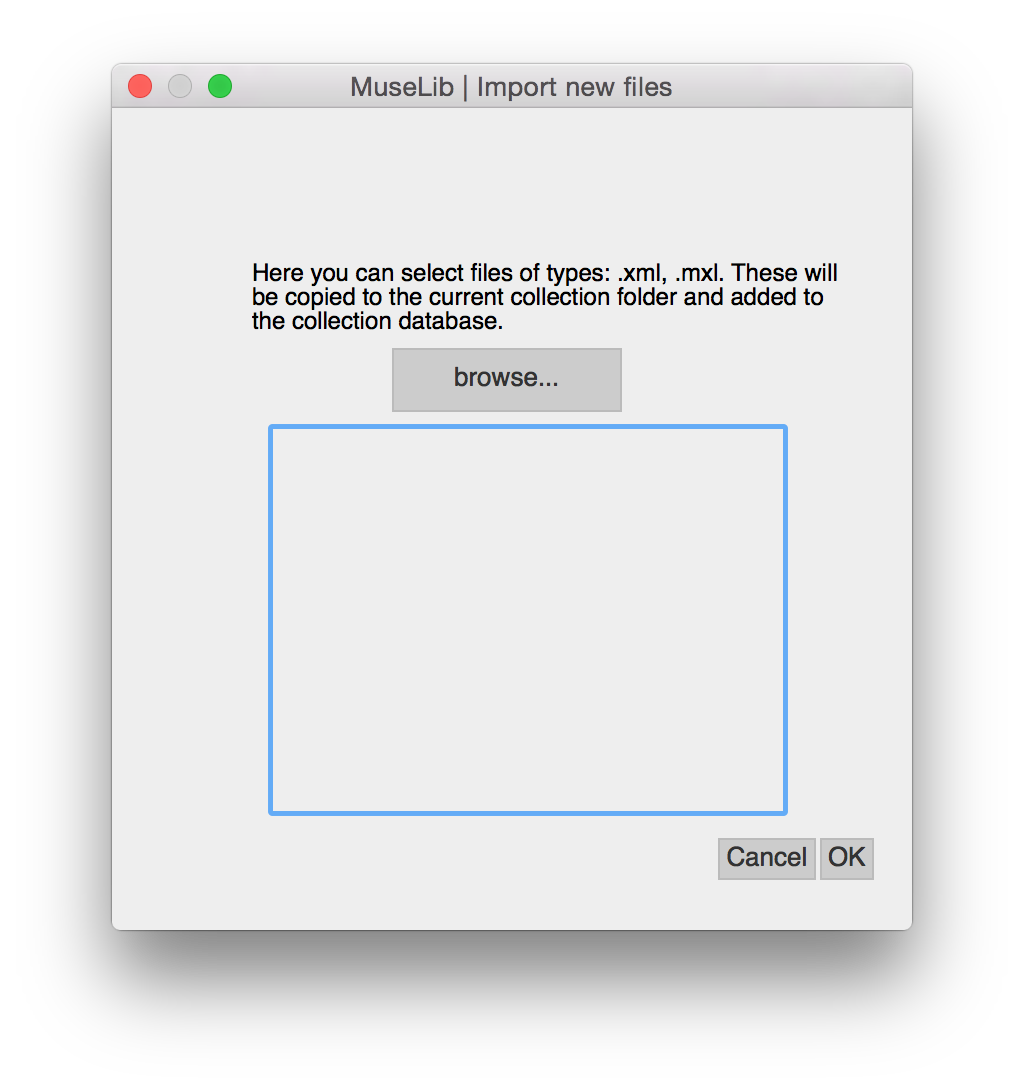
\includegraphics[width=500pt]{importpop}
\caption{The import popup window}
\label{fig:import}	
\end{figure}
Click browse to find the file. This window will allow you to select multiple files by browsing for one, selecting it and then browsing again. The list of files to copy will display in the listbox below the button.


\subsubsection{Error Popup}
Occasionally, files produce problems the system cannot handle - this includes drum tab and guitar tab. At other times there will be problems in the process the application could not process for different reasons, such as downloading files without internet connection. When these occur, the popup in figure \ref{fig:error} will display. If you find any odd errors, please report these to a developer.
\begin{figure}[H]
\centering
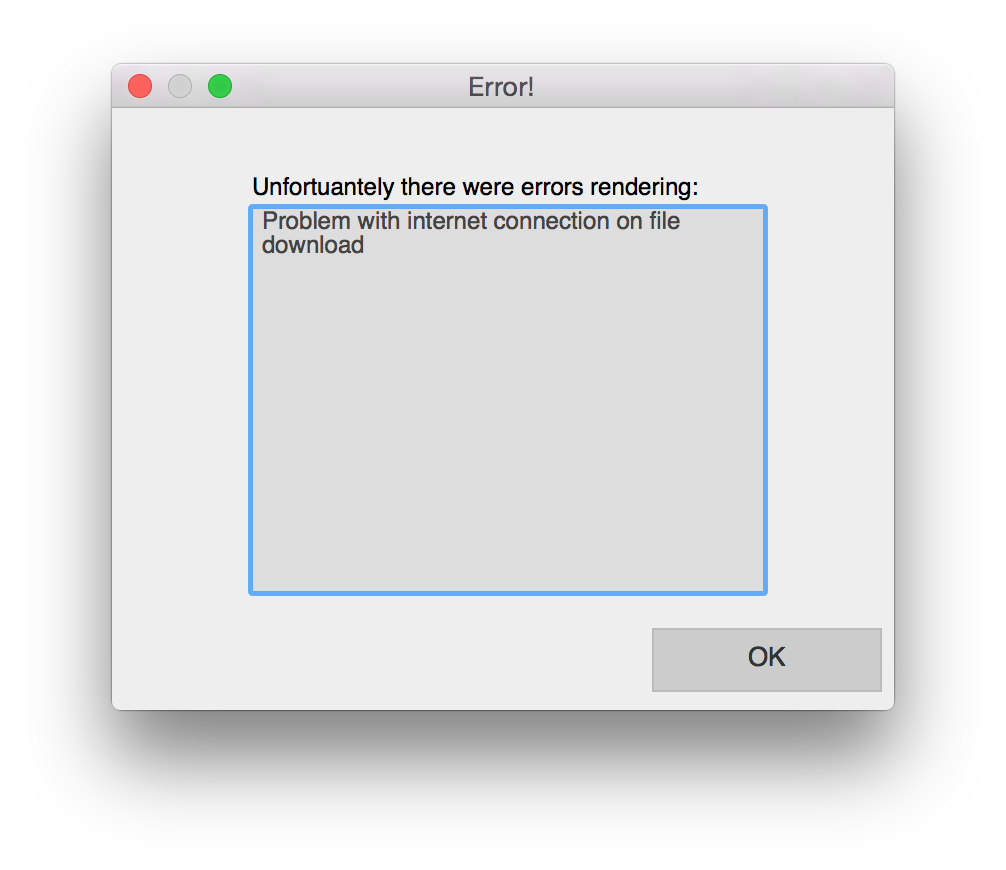
\includegraphics[width=500pt]{errorpop}
\caption{The window which will display on startup}
\label{fig:error}	
\end{figure}

\subsection{Customising your display}
\subsubsection{Themes}
The system comes with three different themes - the default which is light, dark and electric blue. These can be changed by clicking them in the theme menu as shown in figure \ref{fig:themes}. Their respective screenshots are shown in figures \ref{fig:theme1}, \ref{fig:theme2}, \ref{fig:theme3} and \ref{fig:theme4}.
\begin{figure}[H]
\centering
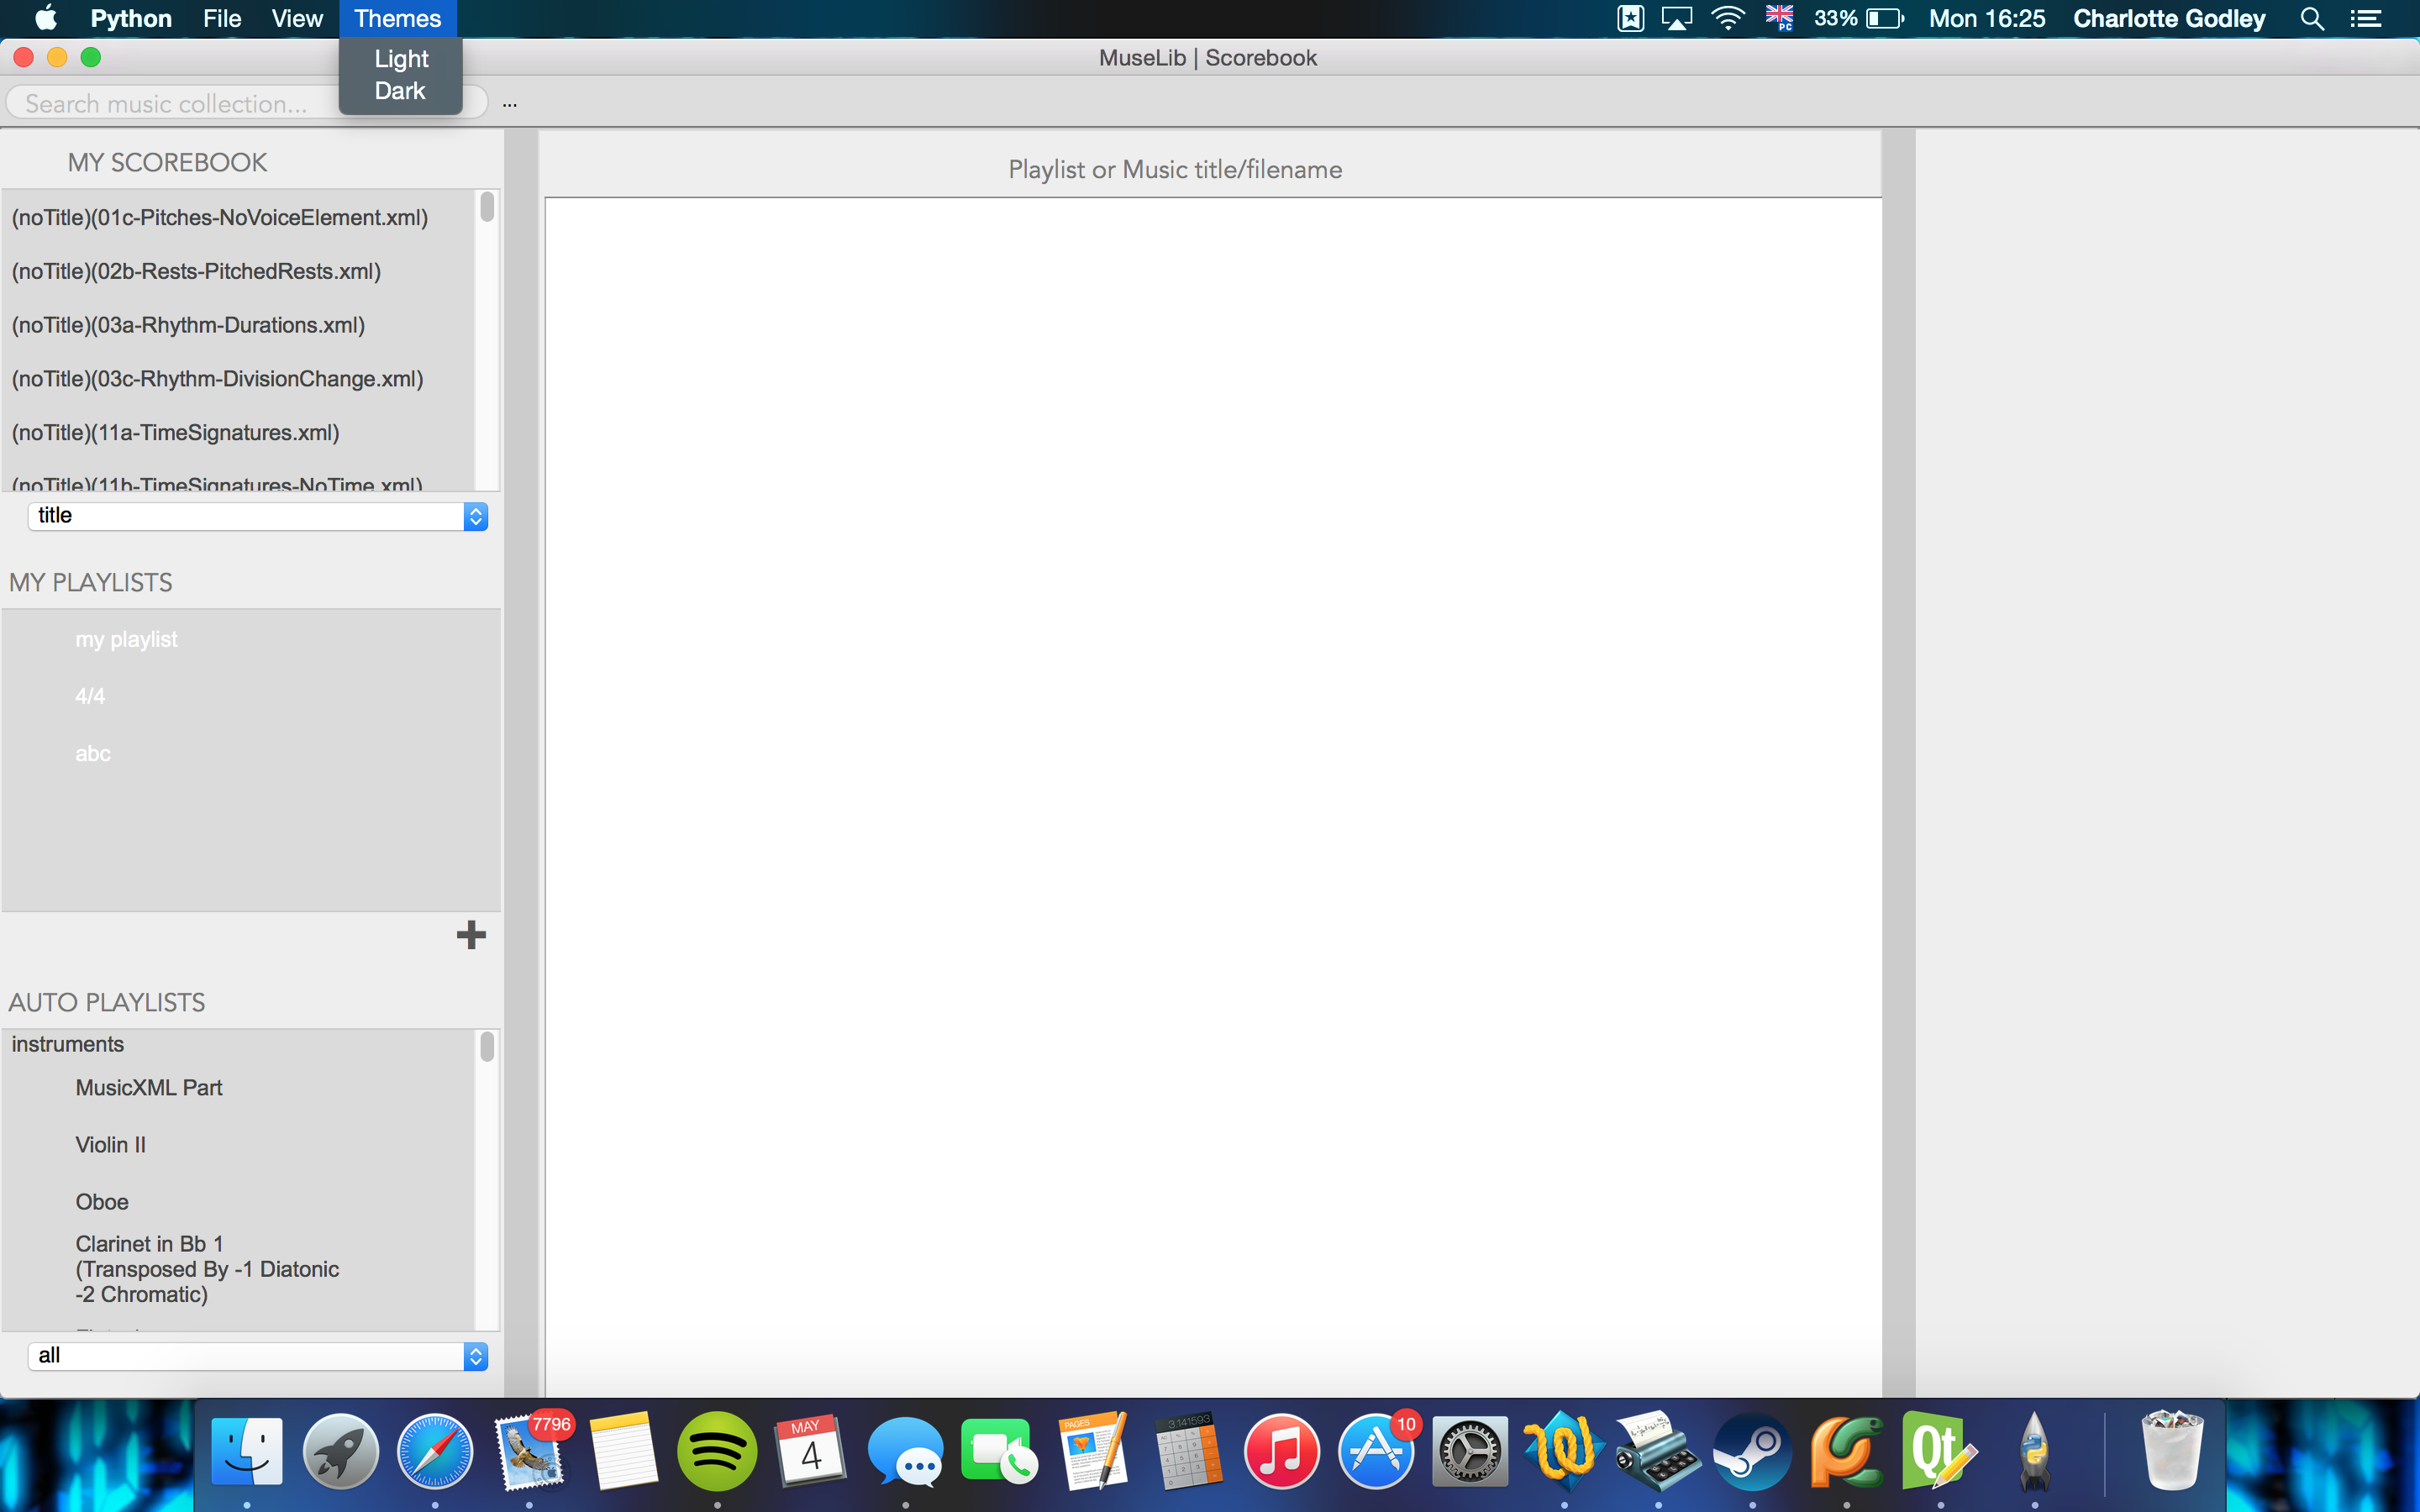
\includegraphics[width=500pt]{theme}
\caption{The themes menu}
\label{fig:themes}	
\end{figure}

\begin{figure}[H]
\centering
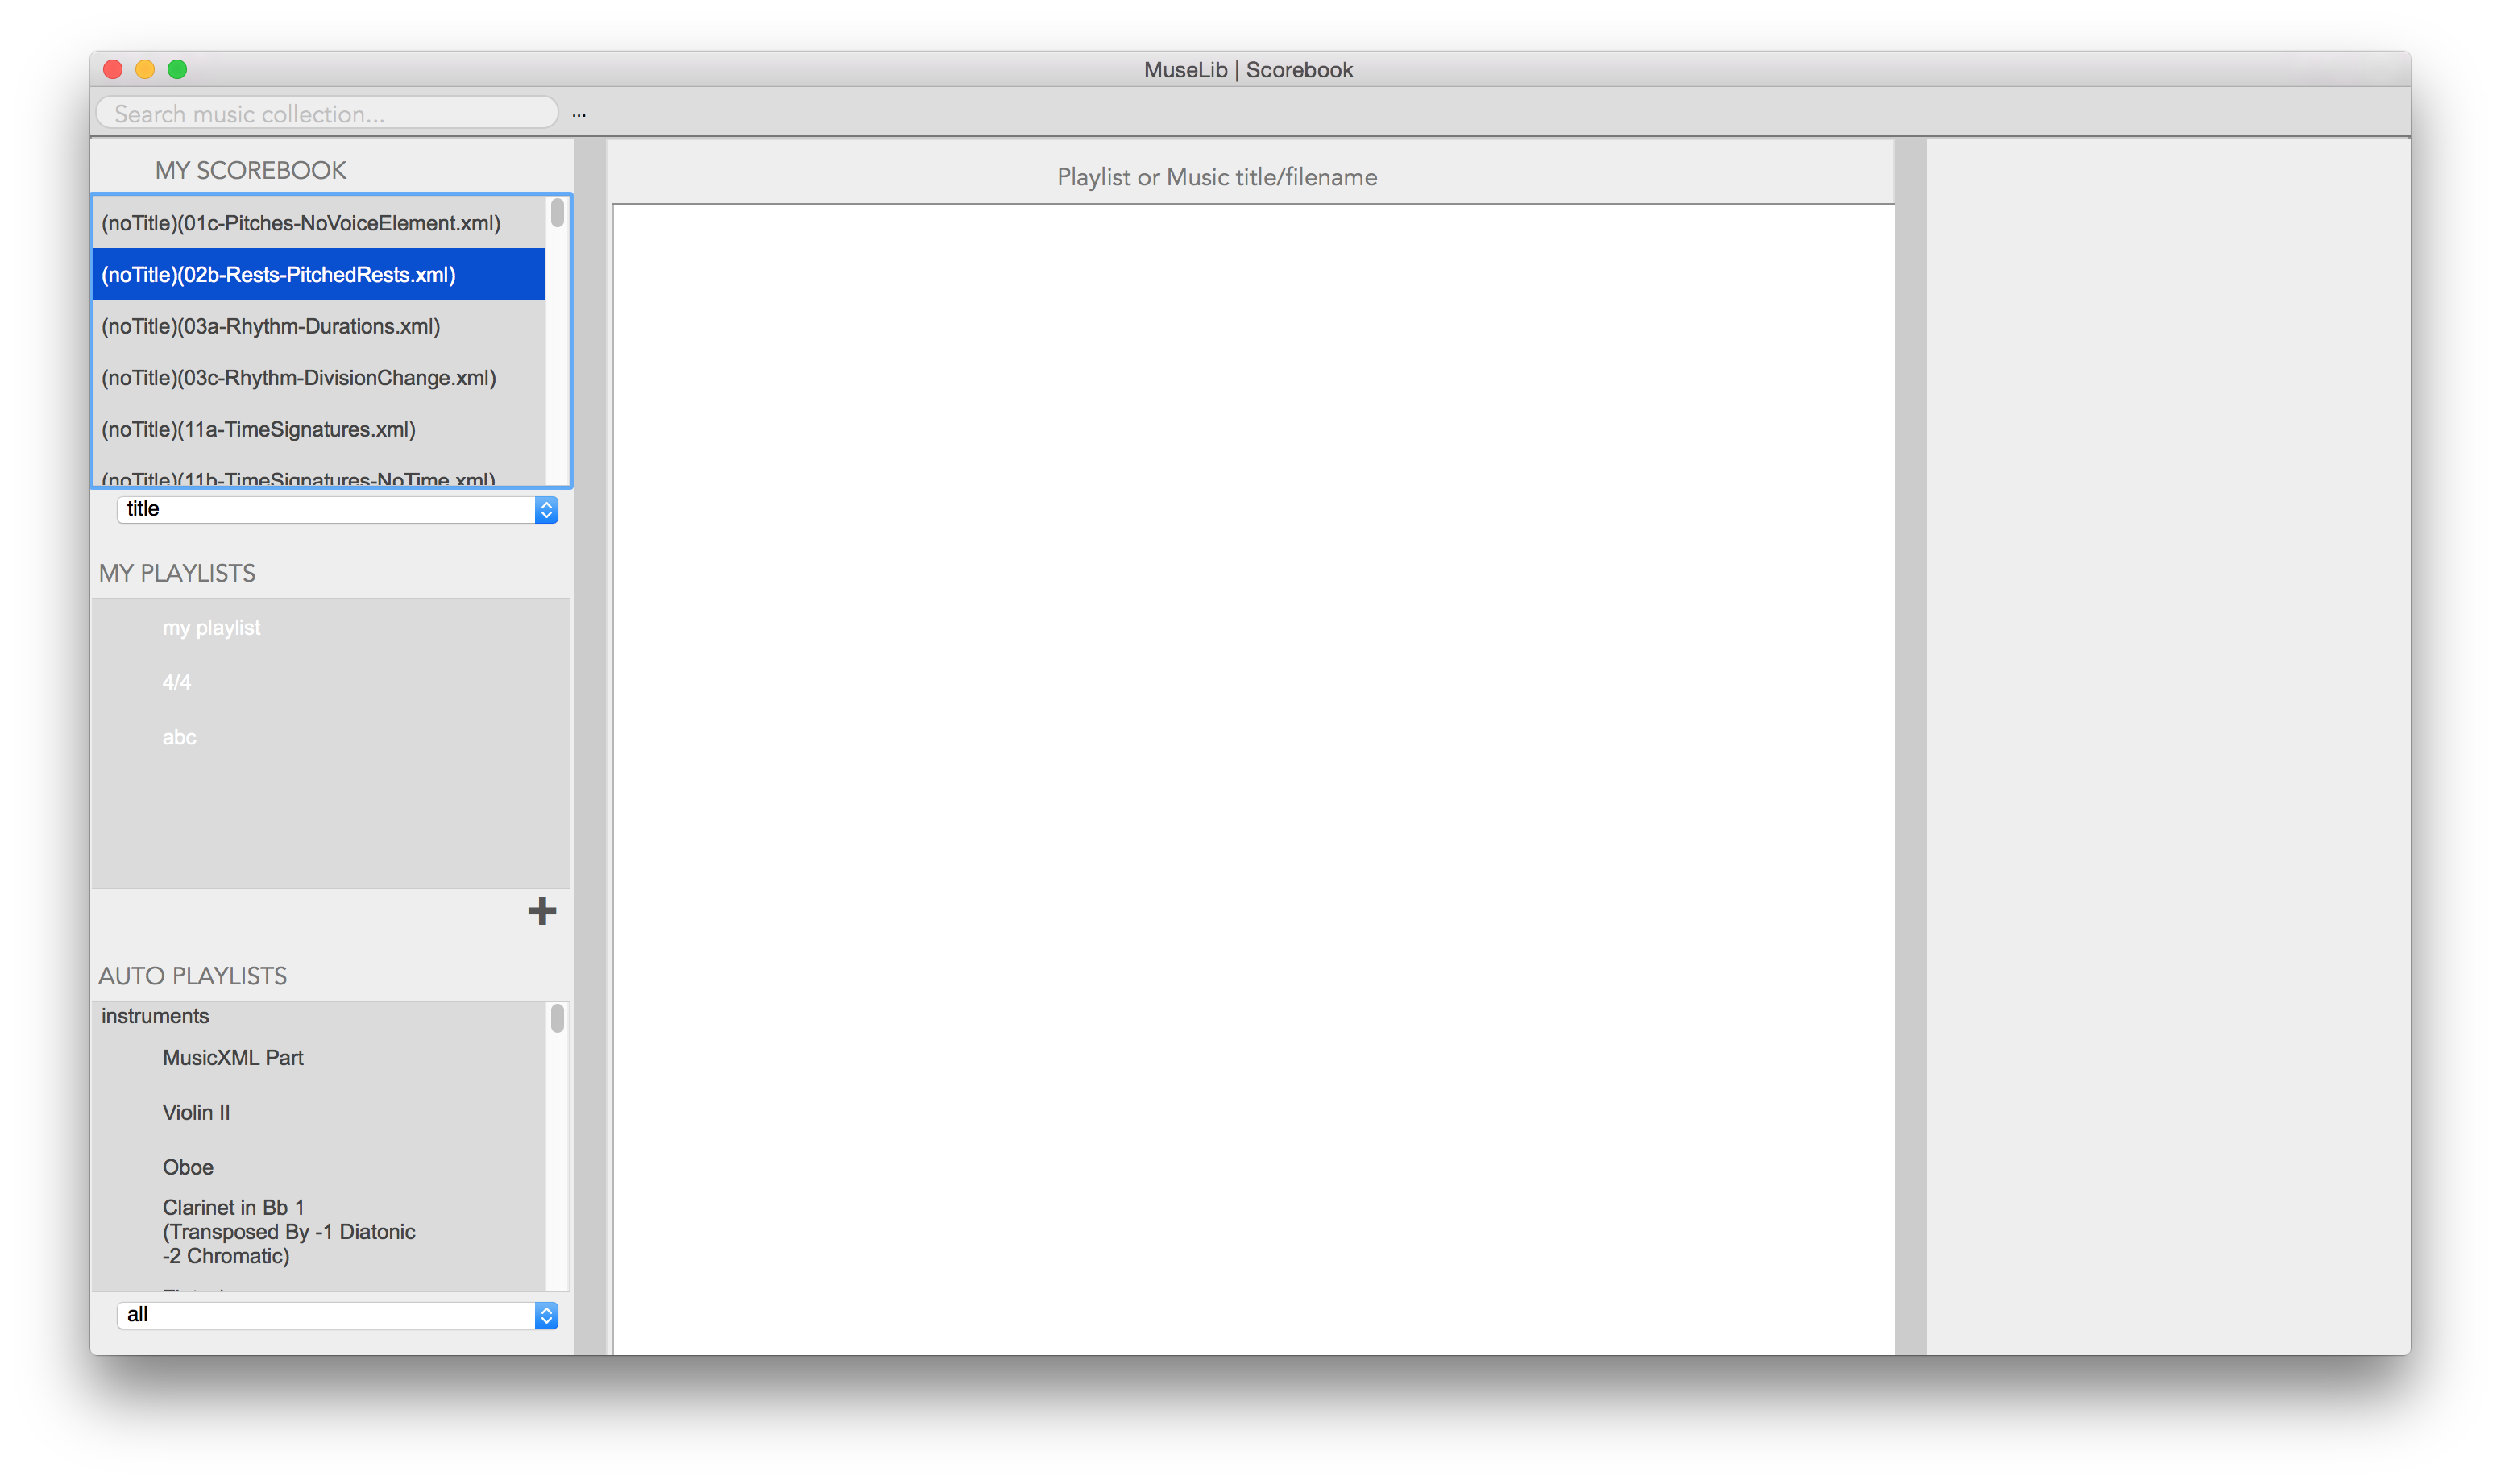
\includegraphics[width=400pt]{main_screenshot}
\caption{The light theme}
\label{fig:theme1}	
\end{figure}

\begin{figure}[H]
\centering
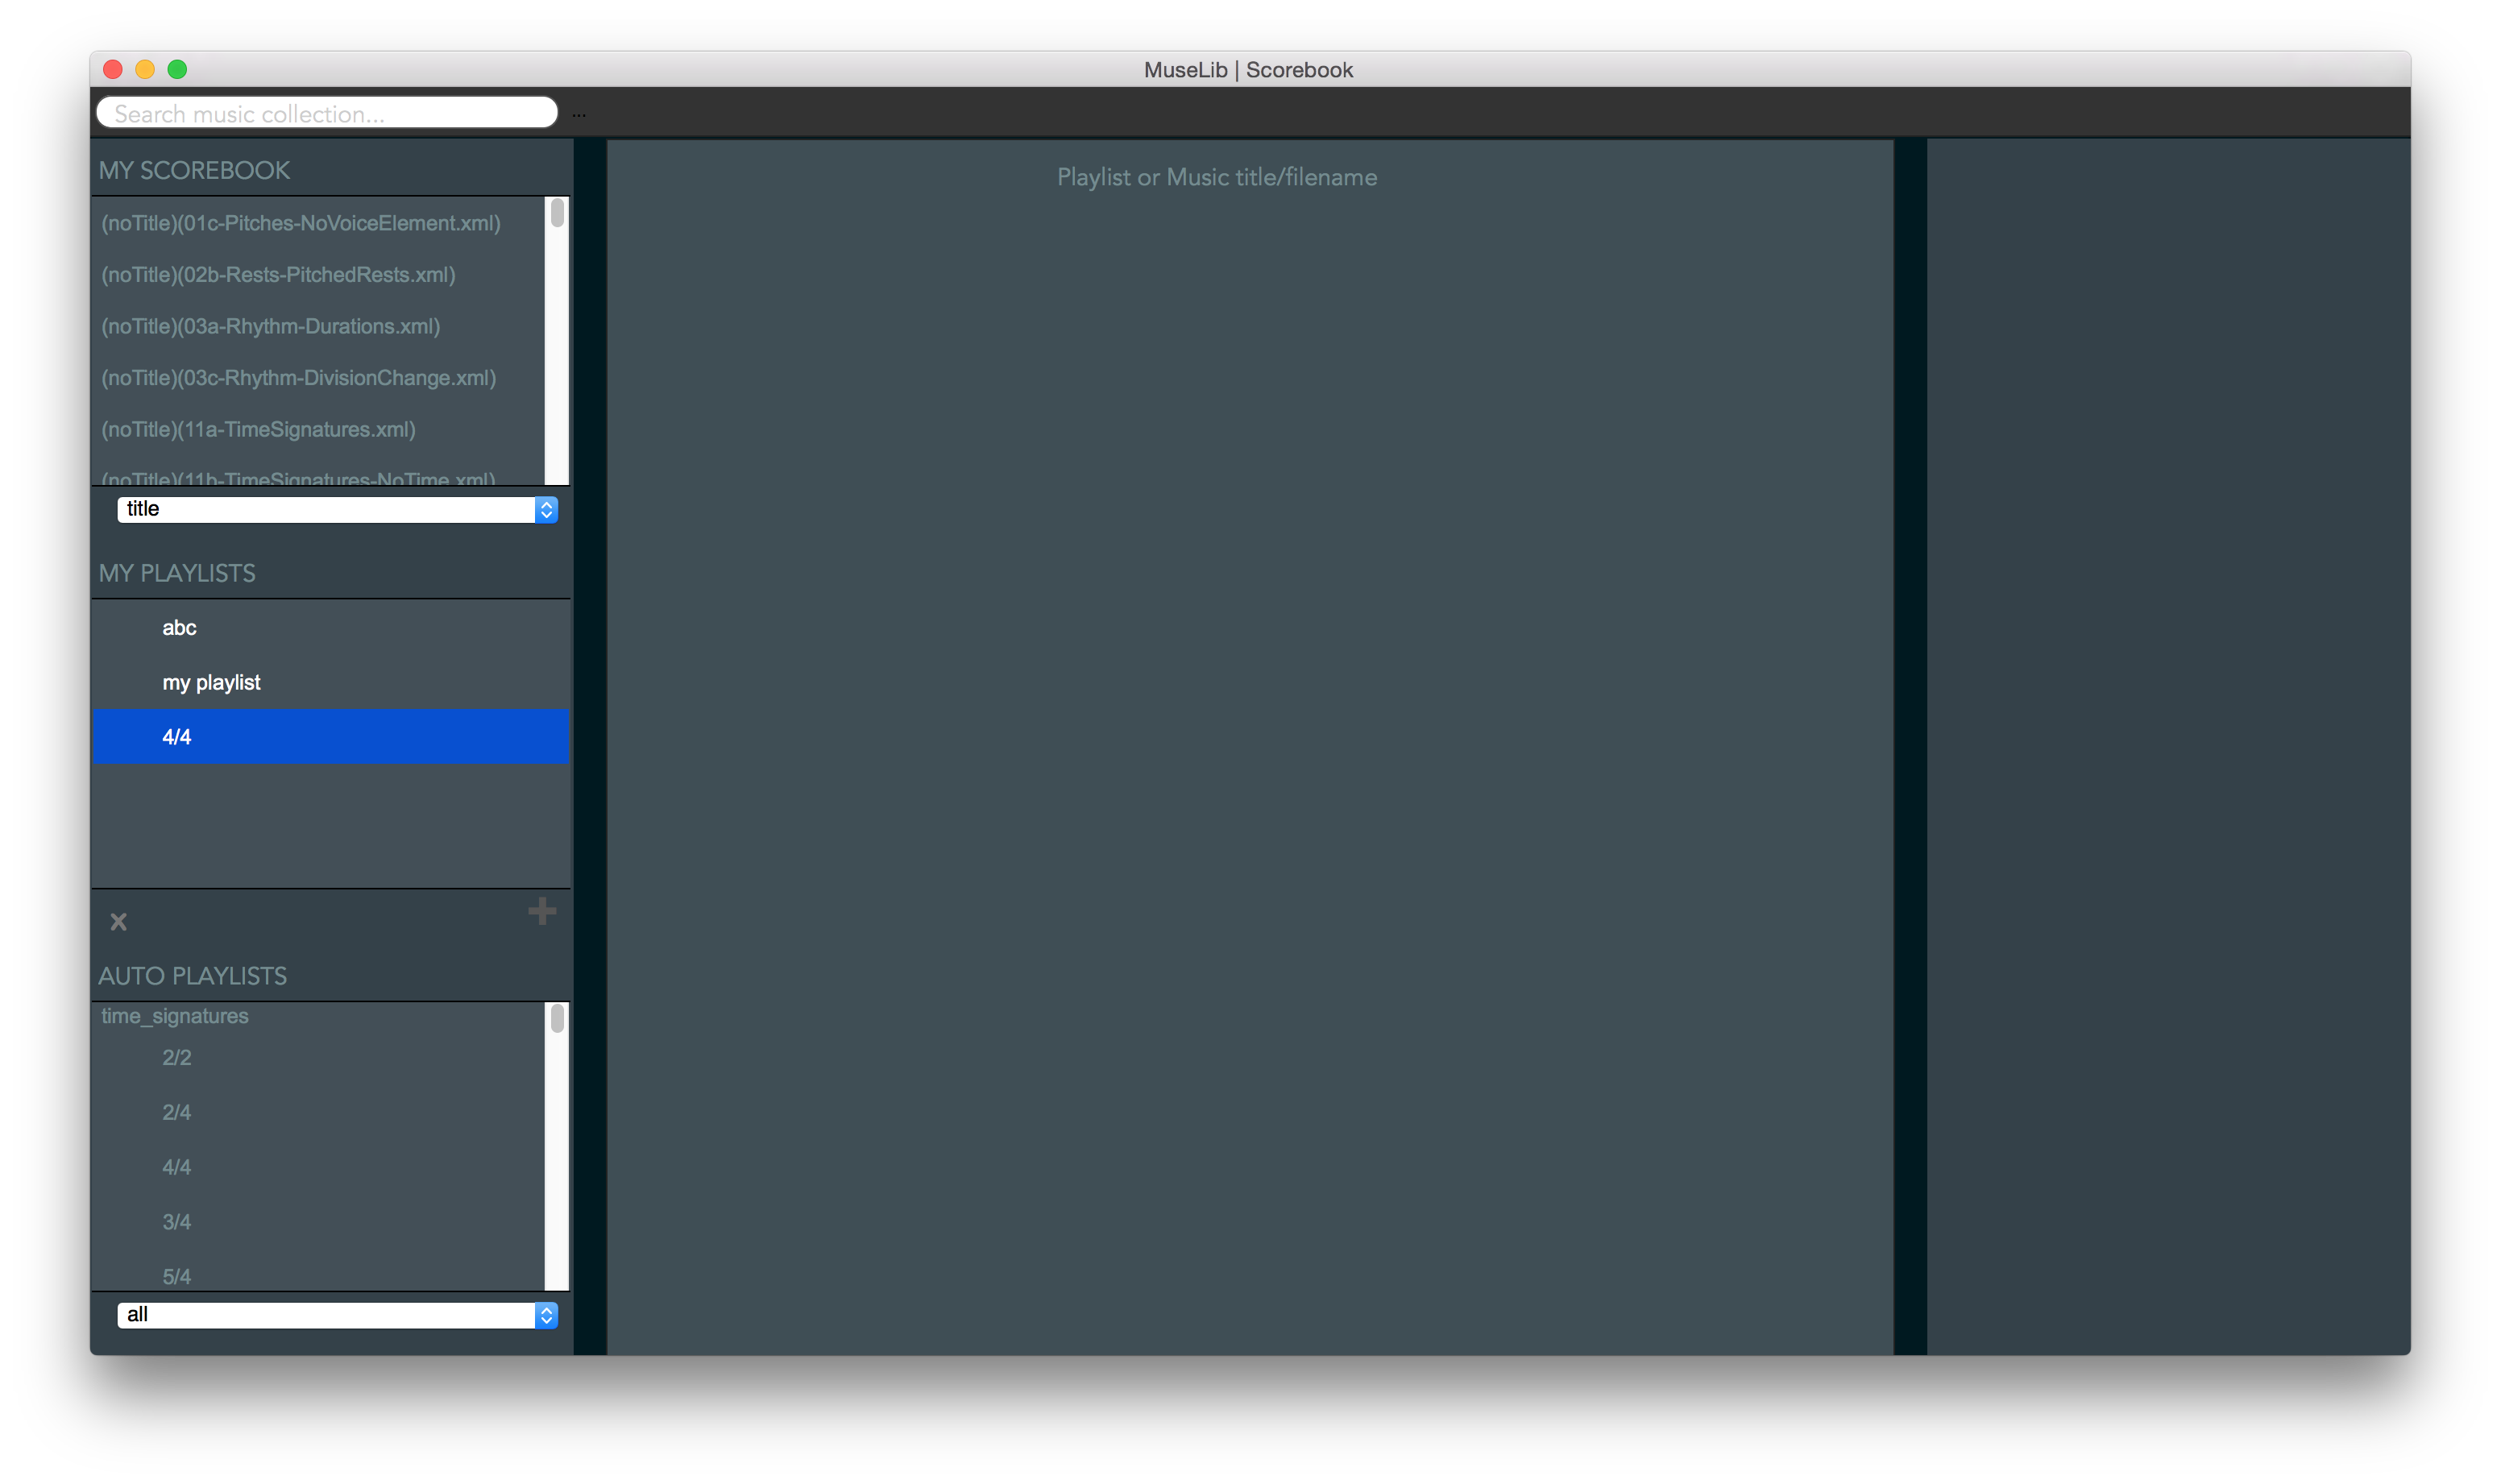
\includegraphics[width=400pt]{main_dark}
\caption{The dark theme}
\label{fig:theme2}	
\end{figure}

\begin{figure}[H]
\centering
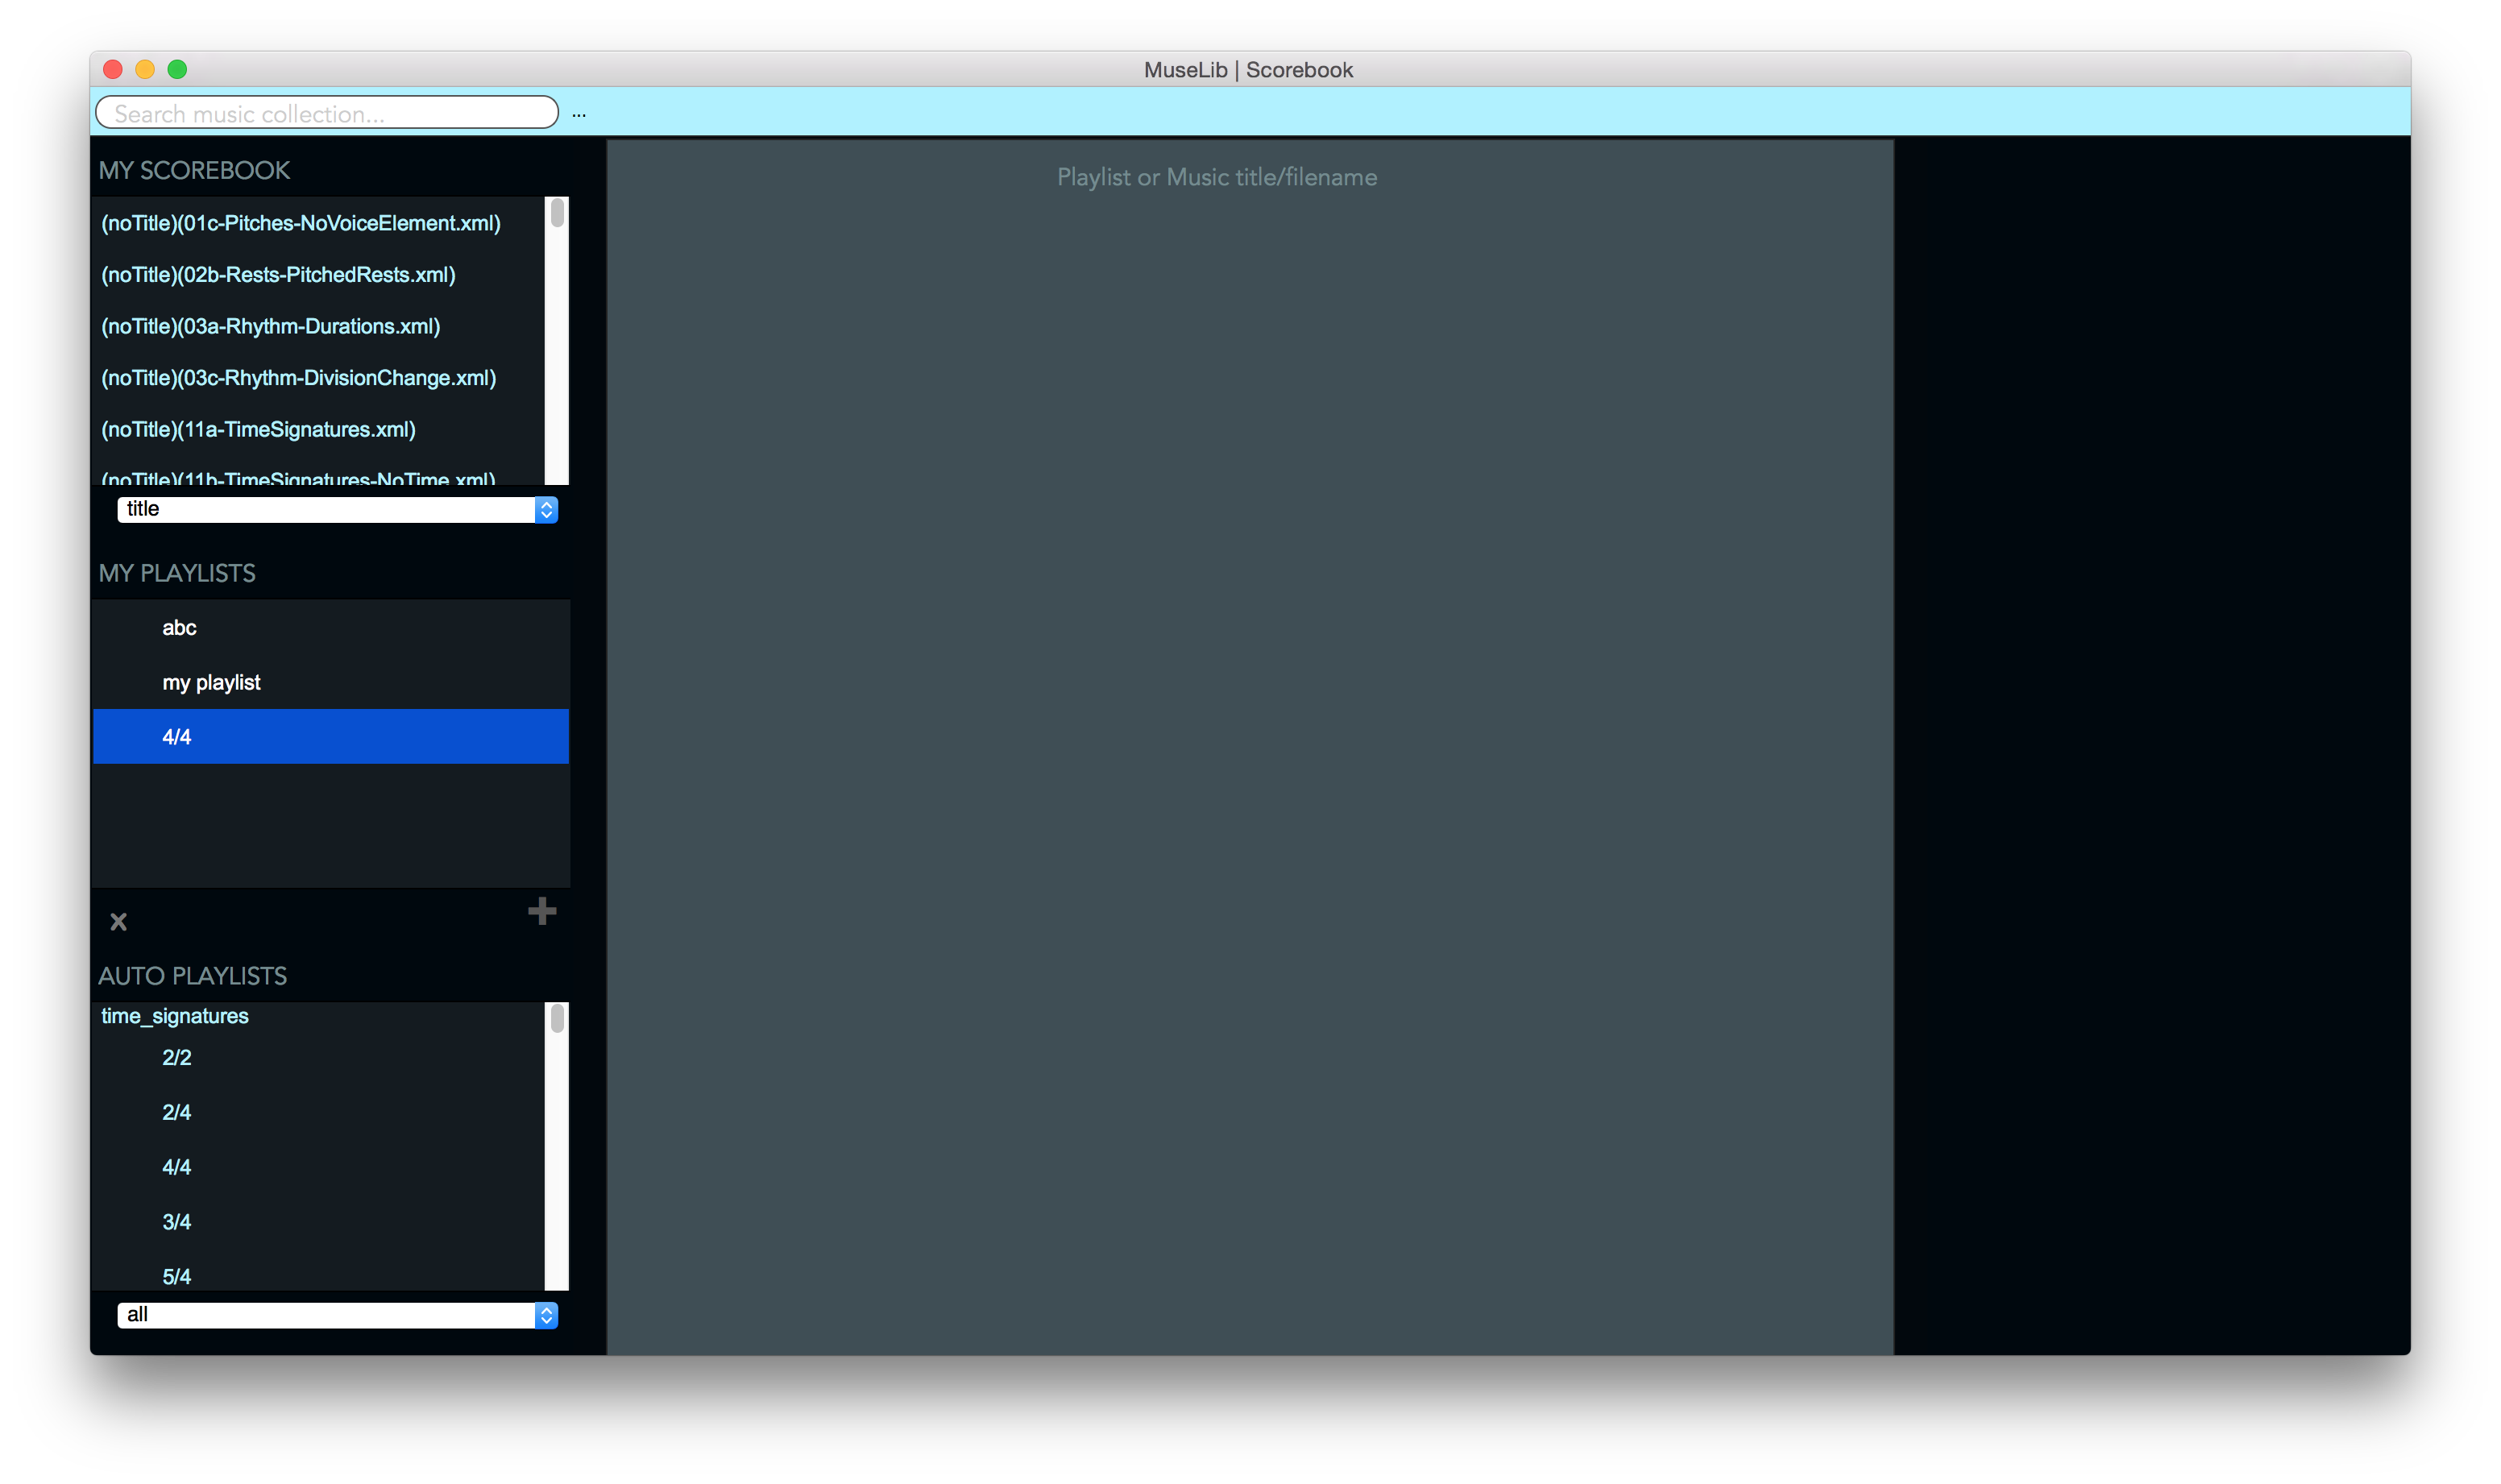
\includegraphics[width=400pt]{main_electric}
\caption{The electric blue theme}
\label{fig:theme3}	
\end{figure}

\begin{figure}[H]
\centering
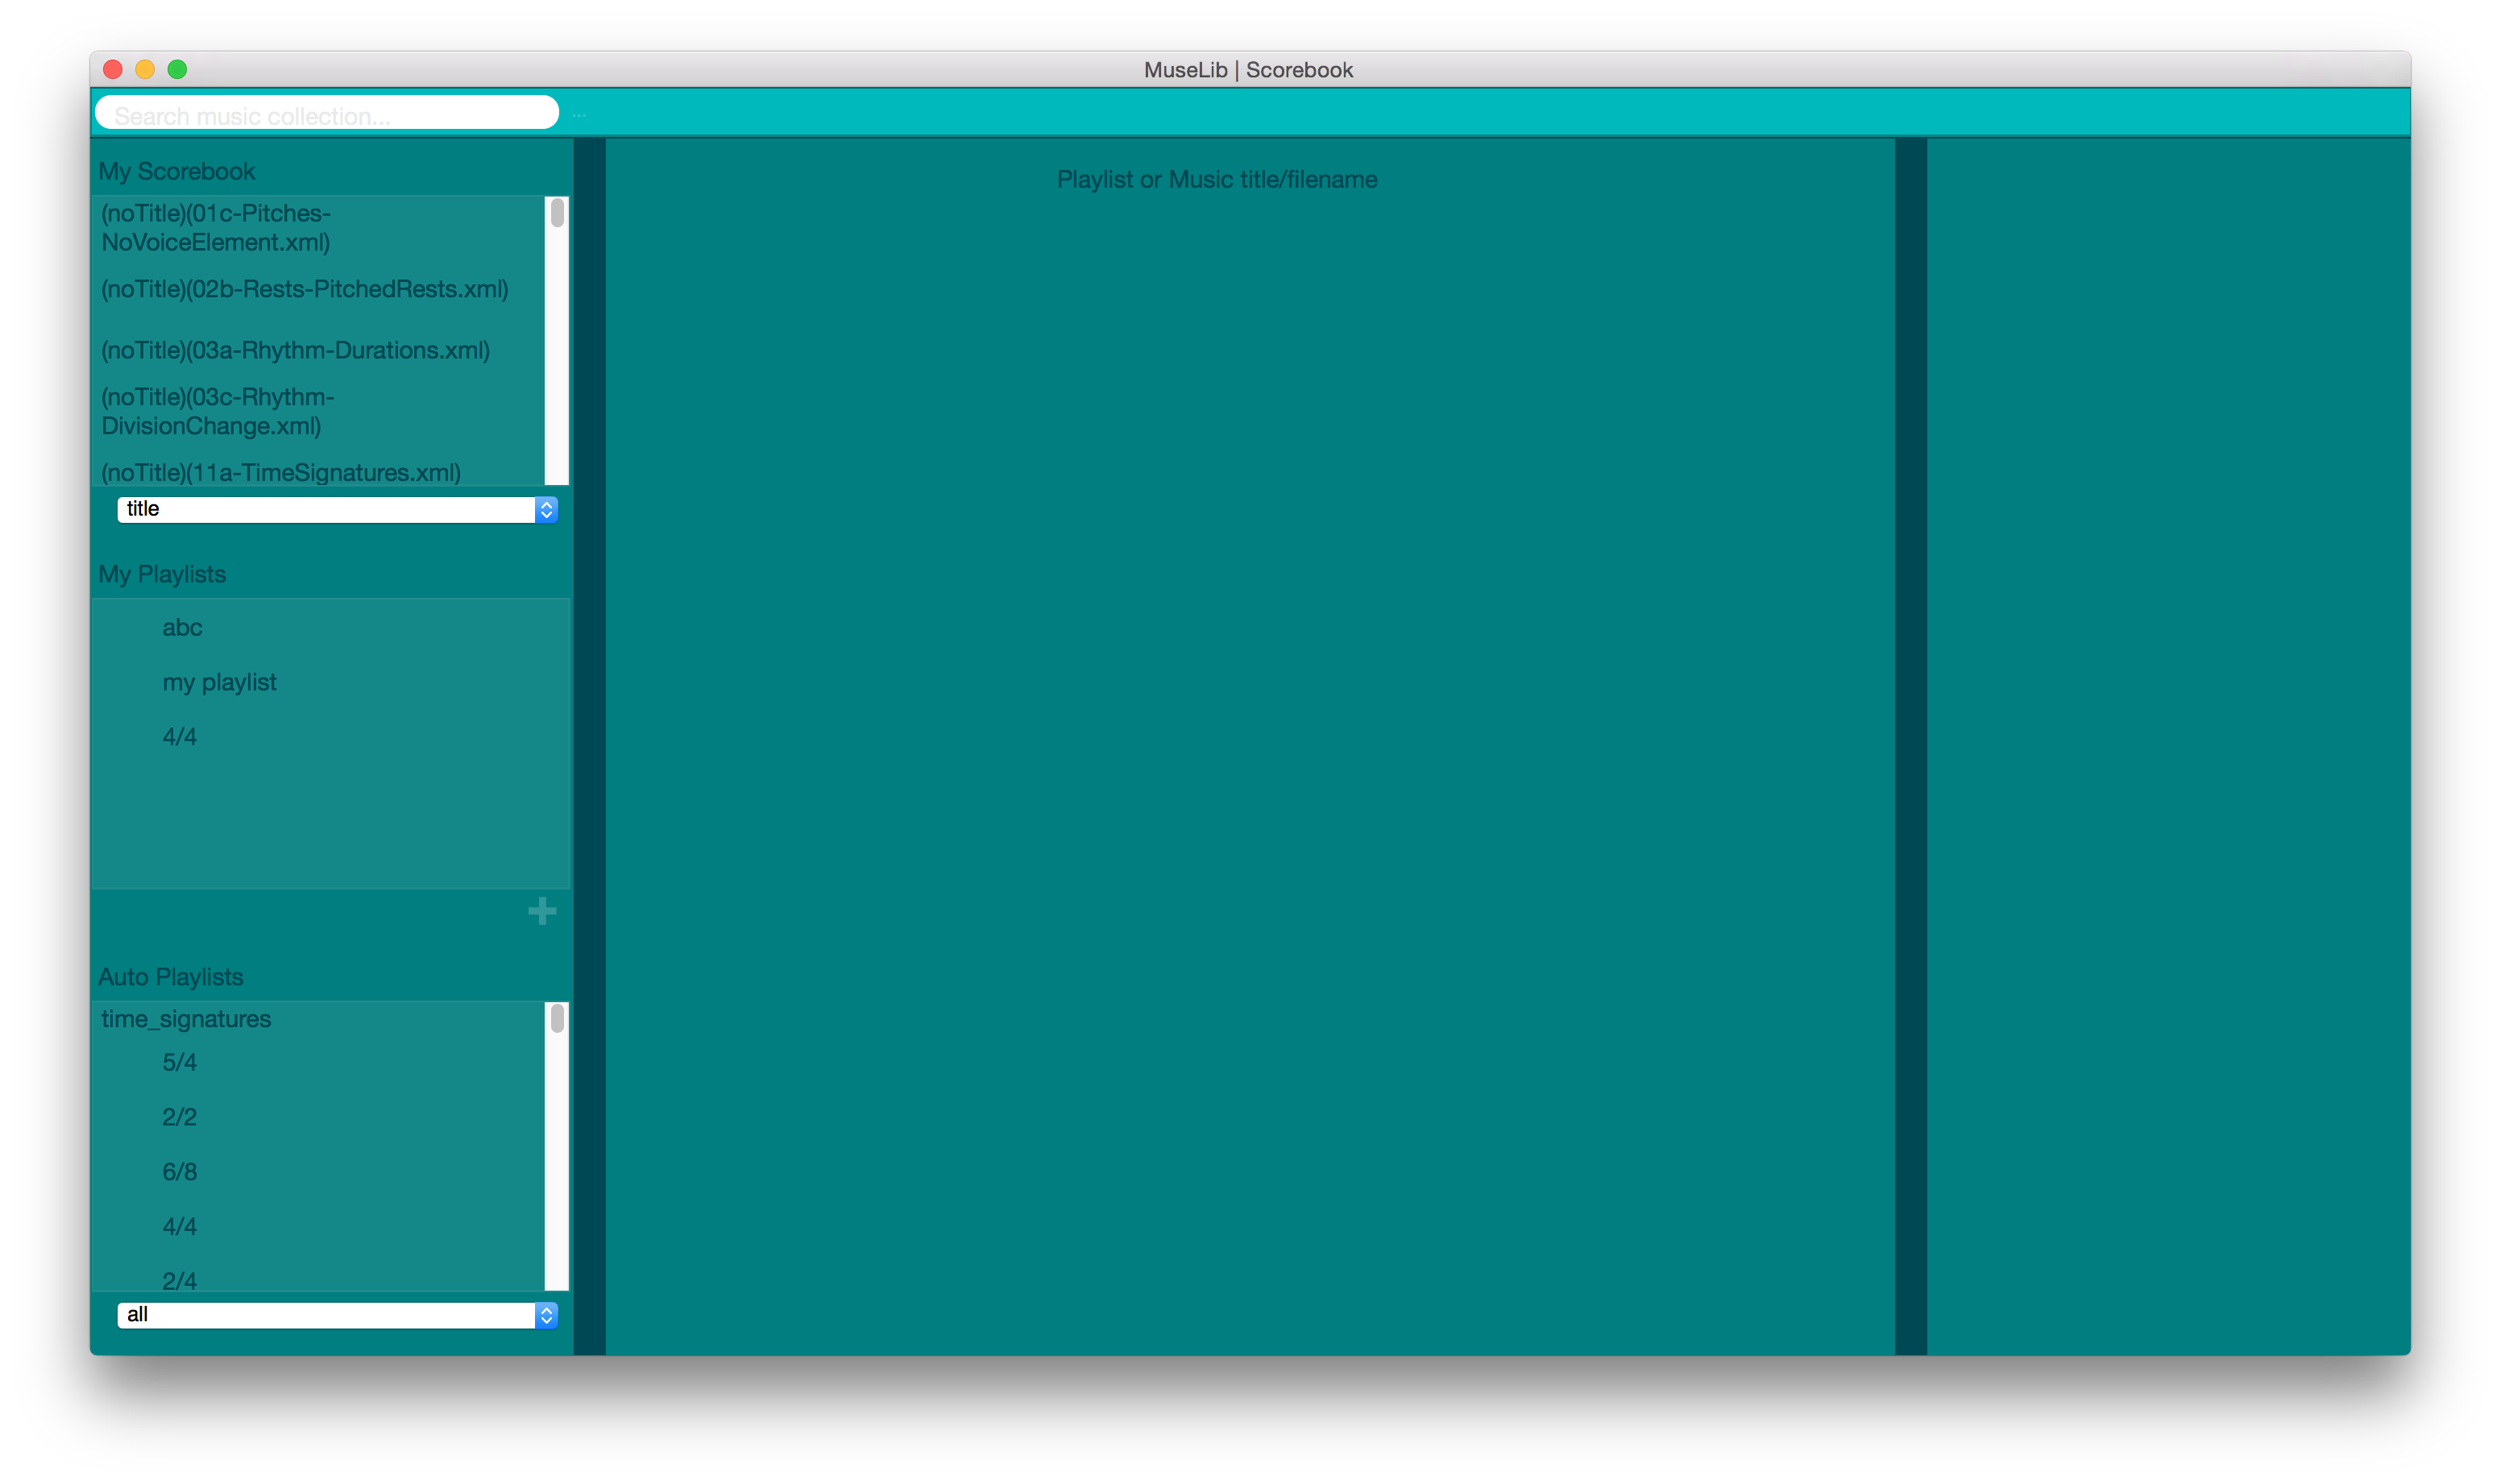
\includegraphics[width=400pt]{teal}
\caption{The teal theme}
\label{fig:theme4}	
\end{figure}

\subsubsection{Customising your widget views}
Any and all of the widgets to the right and left of the main pane can be hidden or displayed using the View menu, as shown in figure \ref{fig:view}.

\begin{figure}[H]
\centering
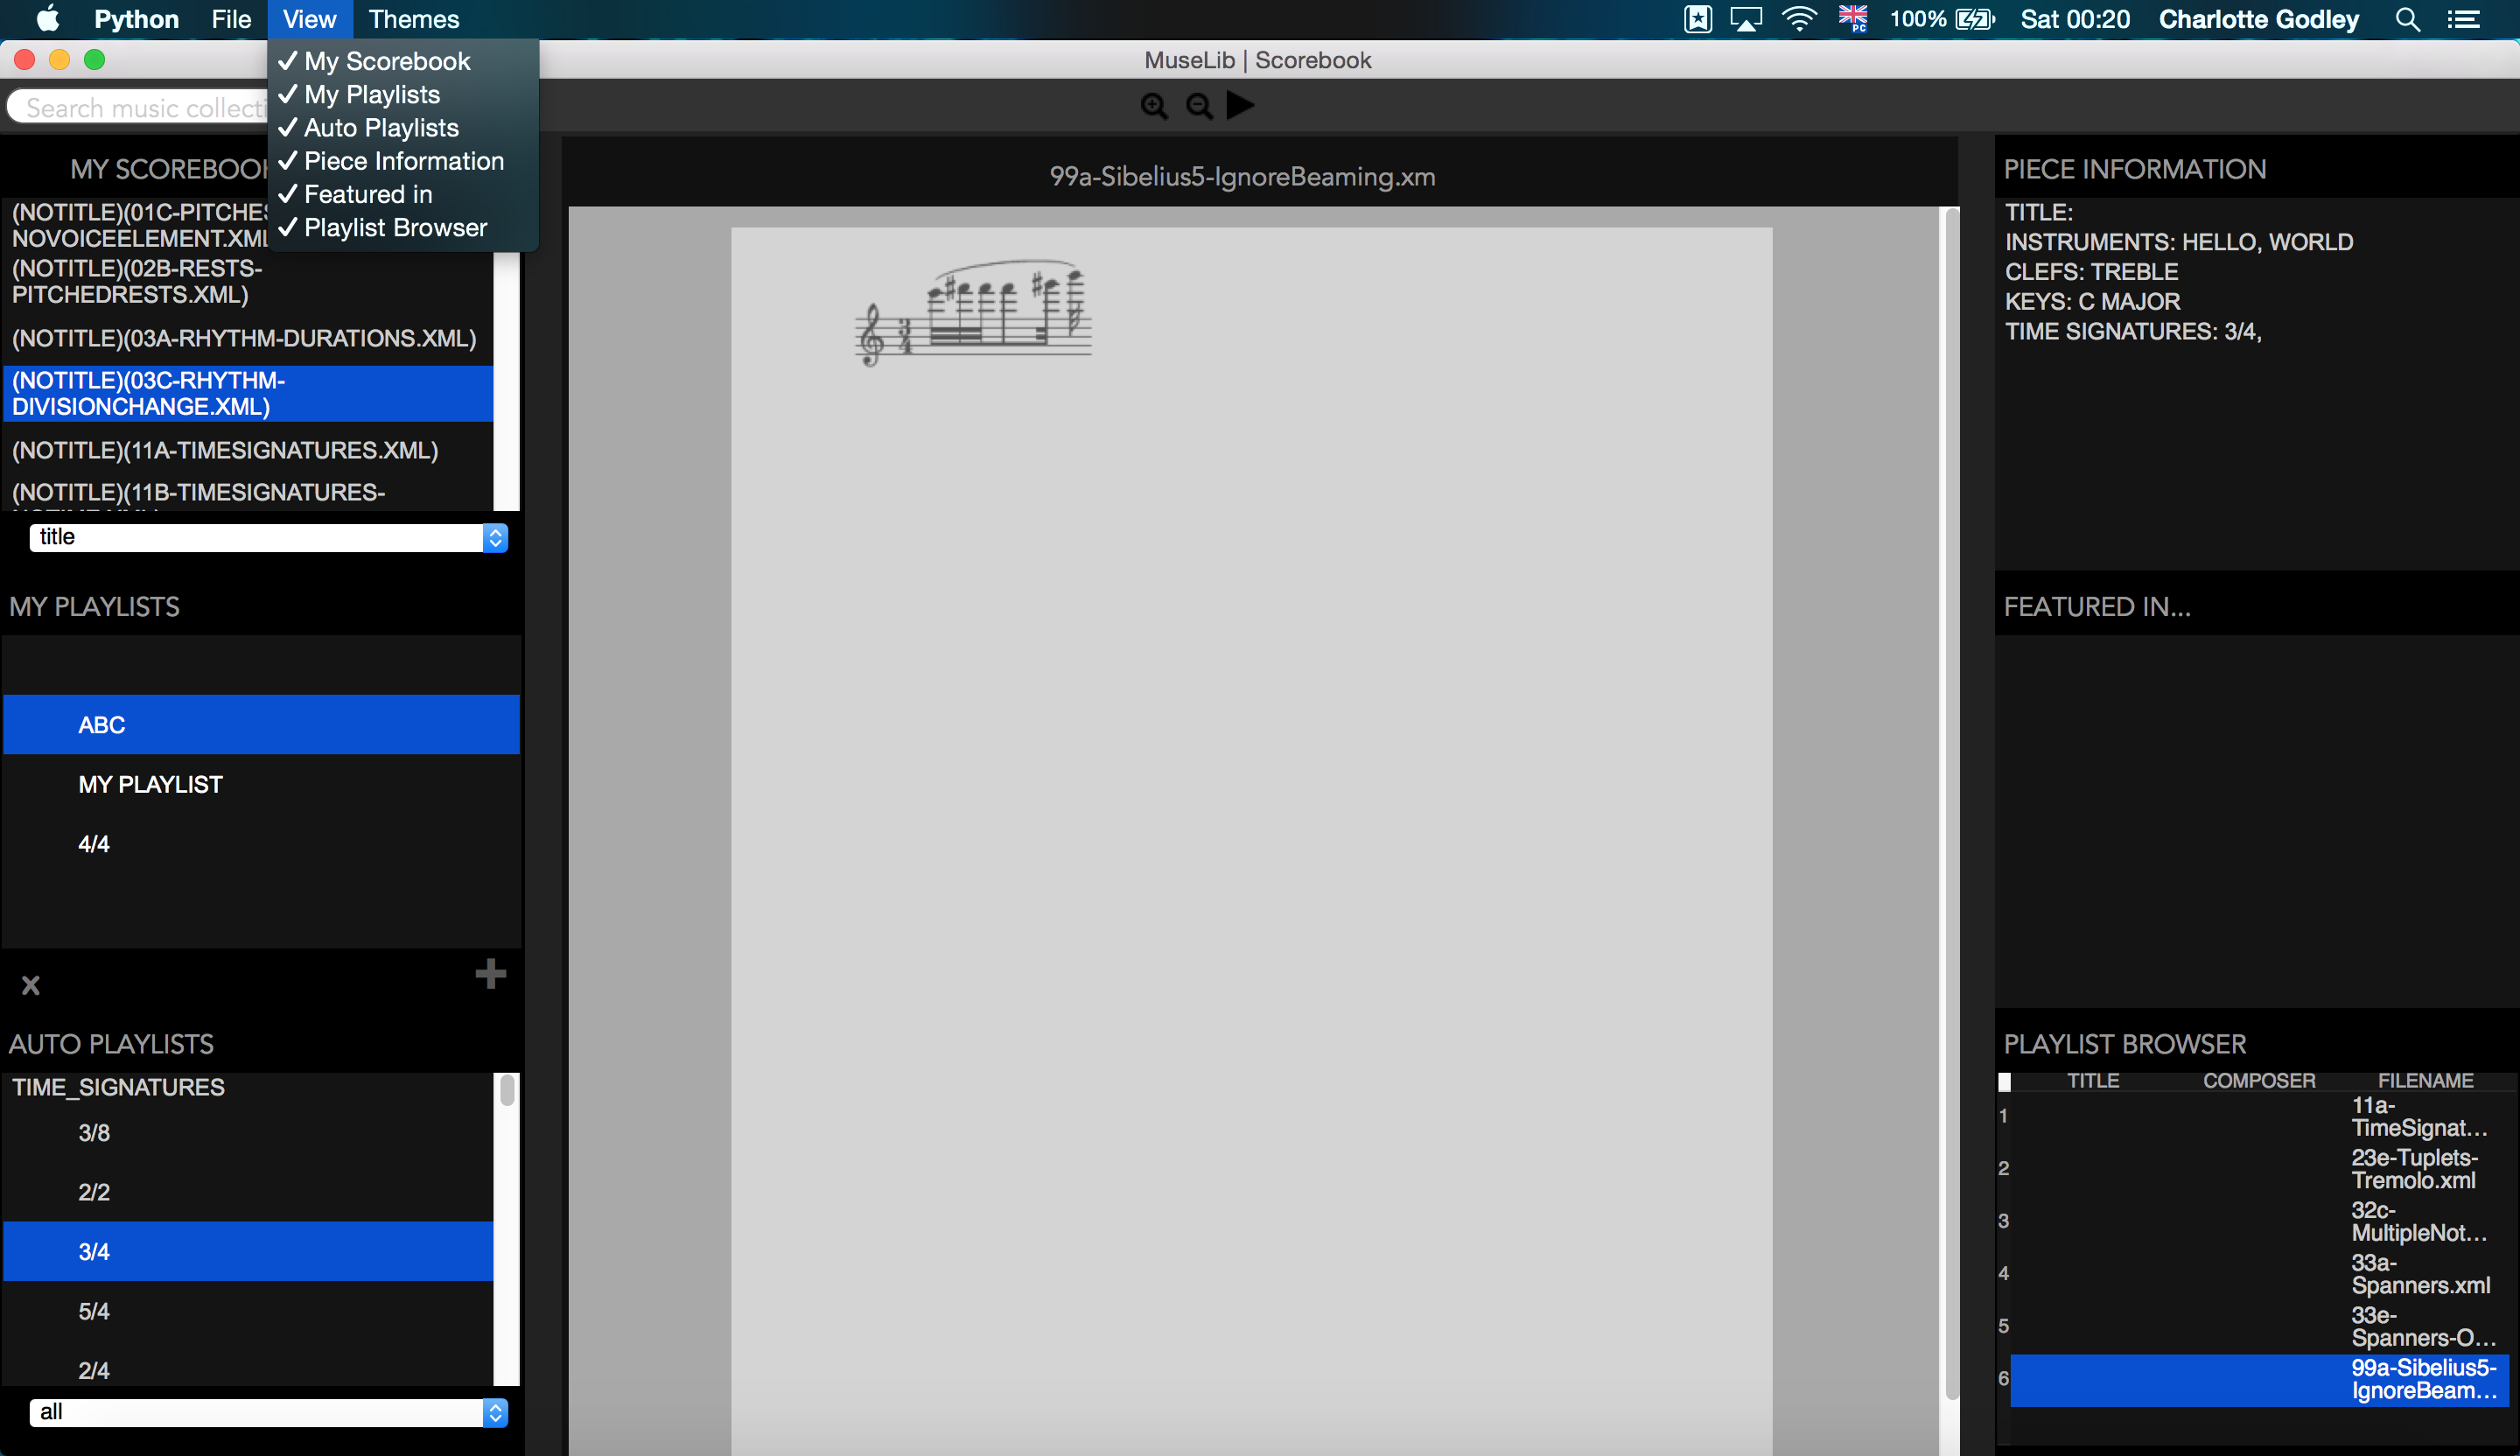
\includegraphics[width=500pt]{view}
\caption{The view menu}
\label{fig:view}	
\end{figure}



\section{Background}
\subsection{Problem Context}
This problem's main focus is the difficulty of organising classical sheet music, and how this can be made easier by the automatic extraction of key pieces  of information. In order to understand what a performer may want to know about a particular piece, it is important to have a brief understanding of the elements of musical notation common to all compositions.

The key element of this form of notation is the staff, as shown in figure \ref{fig:staff}. This is a grouping of five horizontal lines, with each line or space in the staff indicating a different sound pitch, a term meaning the relative "highness" or "lowness" of the sound \parencite{classroom}.

\begin{figure}[h]
    \centering
        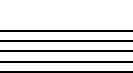
\includegraphics{staff-crop.pdf}
    \caption{A blank staff}
    \label{fig:staff}
\end{figure}

This staff is divided by bar lines, vertical lines delineating grouped units of sound and silence (formally referred to as notes and rests), which provides an indication of the unit's relationship in time by its juxtaposition to other groupings in the composition. These groupings are called measures or bars, with each bar having a variable maximum of notes and rests. 

\begin{figure}[h]
    \centering
        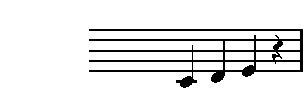
\includegraphics{bar_with_notes-crop.pdf}
    \caption{A bar containing three notes and one rest}
    \label{fig:staff-notes}
\end{figure}
\subsubsection{Clefs}
In the system of staff notation, sound frequencies, or pitches, are denoted by letters A-G - after each cycle of the letter names, the next pitch above it will be the start of a new cycle. The cycles are often split by octaves, a term meaning eight pitches, for example A to A or E to E. 

In order to provide a link between the lines and spaces of a staff and pitch name, a clef symbol is necessary.
\begin{figure}[h]
    \centering
        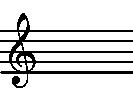
\includegraphics{clef-crop.pdf}
    \caption{A staff with a treble clef}
    \label{fig:clef}
\end{figure}

Each clef symbol denotes a different pitch name - figure \ref{fig:clef} shows a G. The center around which this symbol is drawn - in figure \ref{fig:clef}, the second line from the bottom of the staff - indicates that this line or space will be known as the pitch name denoted by the symbol. From this the reader can infer all other pitches by counting through the letters of the cyclic octave system, so in figure \ref{fig:clef}, the space above becomes an A, and the space below becomes an F.

This symbol is important to a musician as different clefs are used to position the majority of the pitches in a piece on the staff, as this makes it easier to read. From this a performer can infer the average range of a piece, and predict whether this will be comfortable for the performer's chosen instrument or voice.

\subsubsection{Keys}
A second important indication to the player is the key, denoted by a key signature.
\begin{figure}[h]
    \centering
        
\includegraphics{key-crop.pdf}
    \caption{A staff with a key signature}
    \label{fig:key}
\end{figure}

The key signature is a collection of symbols at the beginning of the piece which indicate which pitches should be raised by half pitches, and which should be lowered. Raised pitches are called sharps, indicated by the \# symbol, whilst lowered pitches are called flats, indicated by the $\flat$ symbol. Each key, which has a letter name and key type (which can either be "major" or "minor"), has a different combination of flats or sharps. 

This is a useful piece of notation to a musician as pieces in less common keys, such as C\# major or F\# major, may prove more difficult for the user to perform, and therefore they may want to filter out pieces in these particular keys. Similarly, in the case of singers, a singer's range may sit comfortably in one or two keys and they would perhaps want to find pieces in only these keys. 

\subsubsection{Meter}
The third symbol denoted at the beginning of a measure is the meter or time signature, displayed as two numerals positioned like a mathematical fraction.

\begin{figure}[h]
    \centering
        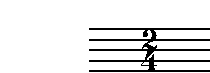
\includegraphics{meter-crop.pdf}
    \caption{A staff with a 2/4 time signature, or meter}
    \label{fig:meter}
\end{figure}

The upper number of a meter symbol indicates the amount of beats in the bar. A beat simply refers to a note or rest, and the type of beat is indicated by the lower number. In the case of figure \ref{fig:meter}, 2/4 indicates a measure will contain 2 crotchets, or quarter-length notes. The most common time signature is 4/4, which for this reason is usually denoted with a C in place of the fraction, meaning "Common time".

This information is important as it tells the performer how the rhythm and beat of the piece should be felt, counted and performed, and is useful for searching purposes as different meters give the piece a different feeling, dictating the sort of occasion this piece would accompany. 

For example, 2/4 is commonly used for march pieces, and 3/4 is commonly used for waltzes and dance pieces.

\subsubsection{Tempo}
The speed of a particular piece, or the tempo, is indicated by an equation.

\begin{figure}[h]
    \centering
        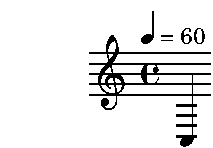
\includegraphics{tempo-crop.pdf}
    \caption{A staff with tempo marking}
    \label{fig:tempo}
\end{figure}

The equation above the staff in figure \ref{fig:tempo} indicates that the piece should be played at 60 beats per minute. The symbol dictating the sort of beat per minute depends on the time signature, here a crotchet (or quarter note) is given as the piece is in 4/4 time. Sometimes, this will be accompanied by a text direction to indicate speed or style, such as Andante, indicating a walking speed.

This indication would prove a useful identifier as pieces of different tempos provide variation in performance lists, so a concert organiser may want to find pieces with a variety of tempos.

\subsubsection{Further metadata}
Aside from these symbols, there are some items of textual information useful to the user. 

The first of these would be the parts in the piece and their transpositions. A part refers to a grouping of measures given to one performer, as shown in figure \ref{fig:parts}. "Part" used in a general sense usually refers to the names given to the left, in this example, "Clarinet in B$\flat$" and "Flute".
\begin{figure}[H]
\centering
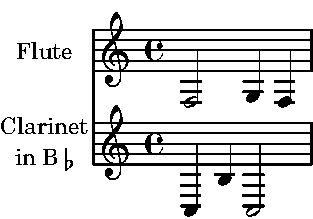
\includegraphics{multiparts-crop}
\caption{Two separate parts in one score}
\label{fig:parts}	
\end{figure}



Parts would be relevant as a particular group of instrumentalists may need parts that fit their instruments. If this is not the case for a given piece, however, a part written for a different instrument, for example, the Alto Saxophone rather than the Tenor Horn, may be compatible with the instrument anyway, if the transposition matches the instruments together. 

An instrument which has a transposition means that, whilst most instruments would play a note as it is written, a transposing instrument will automatically sound the note in a different key, as described earlier, which may raise or lower the sound of the note. For example, the note C played on an Alto Saxophone will sound as an E$\flat$, because it is in the key of E$\flat$ major. 

Further to this, the user would want to know the piece's title, and names of publishers, composers, arrangers and lyricists of the work, commonly known as the bibliography of a piece\parencite{MIR}. Further to the composer name, it may be useful to know the date of composition as an indication of the era in which the piece was composed, such as Classical/Baroque/Romantic, though this would not always be written on the sheet music so may need to be researched using the Internet.

\subsection{Comparison of Technologies}
\subsubsection{Programming Language}
This project could be developed with a variety of programming languages, as displayed in table \ref{table:langs}.

\begin{table}[H]
\centering
\begin{tabular}{| l | l | l | l |} \hline
  {Language} & {Speed of development} & {Developer's Knowledge} & {Most recent use} \\ \hline
  C\# & Fast & A lot & 2nd year \\ \hline
  Python & Fast & A lot & In constant use for over a year \\ \hline
  C++ & Slow & Average & 2nd year \\ \hline
\end{tabular}
\caption{Table of languages considered}
\label{table:langs}
\end{table}
The first language in consideration is C#. C# is mostly used on Windows due to the main compiler being closed source, but with some platform independence due to the Mono Project, which is feature-complete to C\# 10 \parencite{MonoDev}, or Xamarin Studio and other such tools, but the developer has not developed any applications with C\# for use on multiple operating systems. 

In terms of speed of development, the developer considers that the language syntax is reasonably intuitive and consistent, but that by virtue of the language being statically typed, considerations such as dynamic typing and the need to write more code in terms of key strokes, the second language consideration has the advantage.

Finally, due to the language being mostly for Windows and largely being closed, C# has a lower amount of Open Source projects on the popular Open Source Code Repository Github, as shown by the graph in figure \ref{fig:graph}. Whilst this is not necessarily important to development at this stage, the developer intends to Open Source the project and if there are more repositories for Python, as the graph indicates, this would potentially mean there would be more potential contributors.

\begin{figure}[h]
\centering
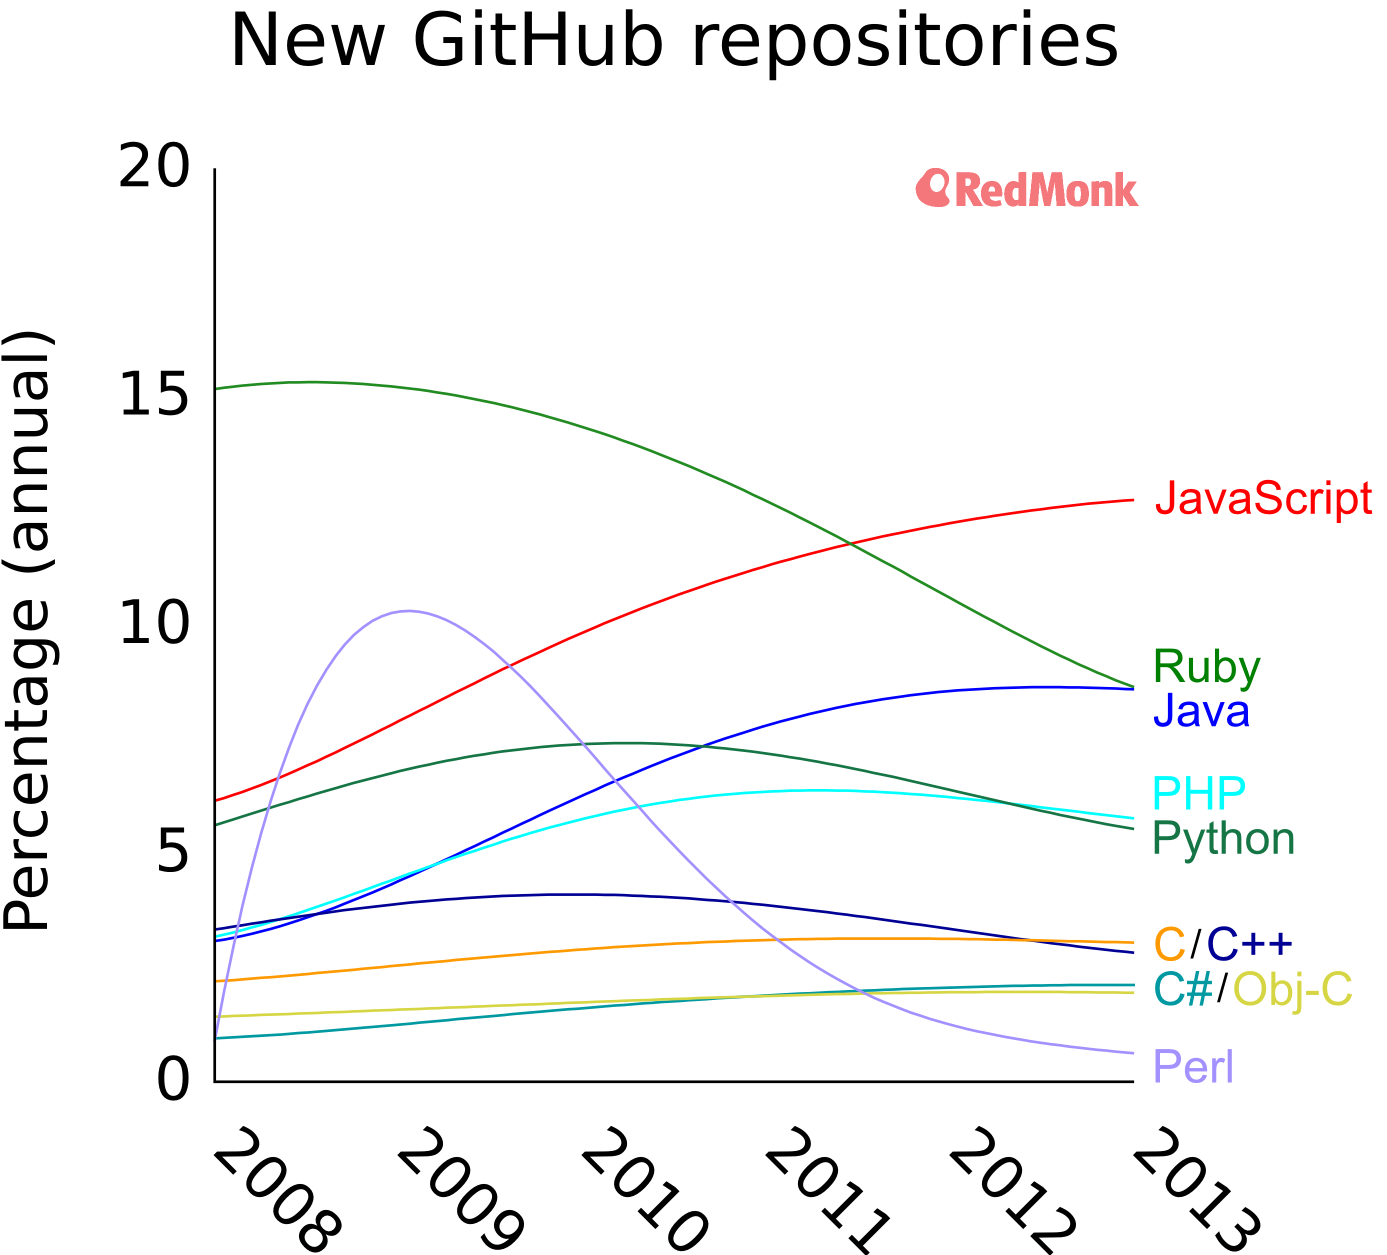
\includegraphics[width=250pt]{github-repos}
\caption{A graph showing the percentage of repositories on Github in different languages}	
\label{fig:graph}
\end{figure}

The second language in consideration is Python. Python is cross platform, as it is included by default in OSX and Linux based Operating Systems with the ability to install it on a Windows operating system.

In terms of development speed and syntax, Python's syntax is the closest of the three considerations to english or pseudocode, and thus requires the least amount of key strokes. Being closer to english also means that the project is more likely to attract a wealth of less technical contributors, in particular musicians, as the language should be easier to learn how to use.

 Furthermore, as it is dynamically typed this allows the developer to use a particular advantage of ducktyping whilst developing, meaning that so long as a class has a particular behaviour, the program can use the class for it's purposes and ignore differences to other classes without implementing an interface.
 
 Lastly, there are many current projects written in Python in the area of Music research \parencite{pmus}, which means the project will be easier to integrate and communicate with other projects or build upon the work of others without needing to port software to Python.

The third and final language in consideration is C++. Whilst C++ is arguably the closest to native code and therefore the language which will be the best for cross platform development, the syntax and memory management issues of C++ mean that development can be slower, particularly when the developer does not feel as competent using this language.

It is for these reasons that Python has been chosen as the development language. Beyond the selection of Python, it is important to discuss and consider which version to use, as Python 3 was introduced in 2008, but Python 2 continues to be maintained and was updated to include many of the backwards compatible features in 2010. Whilst this seems an obvious choice as Python 3 is the latest version, many projects still have issues updating and using Python 3 as it was deliberately not backwards compatible \parencite{Foundation2}.

Upon due consideration, Python 3 has been selected, though if the project requires legacy libraries this may have to be evaluated again. This decision has been made because at this stage the project does not appear to require libraries which do not work with Python 3, and therefore the developer should make every effort to keep the project up to date with the latest version.

\subsubsection{File format}
The project will require at least one default format for it to process music, which needs to have detailed information about what the score contains. Table \ref{table:formats} describes the options considered.

\begin{table}[H]
\centering
\begin{tabular}{| c | c | } \hline
  {\textbf{Format}} & {\textbf{Purpose}} \\ \hline
  muscx & MuseScore notation \\ \hline
  SIB & Sibelius notation \\ \hline
  new format & this project only \\ \hline
  MusicXML & sharing music between software \\ \hline
\end{tabular}
\caption{A table showing the different file formats considered}
\label{table:formats}
\end{table}
The first two options, muscx and SIB files, are formats used by the open source notation software MuseScore \parencite{MuseTour}, and the world's most popular proprietary notation software, Sibelius \parencite{avid}. Using either or both of these files would mean the majority of users would be able to use the application. 
However, both options couple this project with those particular packages, when users could still choose other software to write music with. Furthermore, the formats are specifically designed for those software packages and may have nuances which make development for this project more difficult. Additionally, Sibelius is proprietary so borrowing their file format may cause copyright issues.

The third option is to create an entirely new format. This would mean the file format was designed to the requirements of the project and therefore be entirely customisable and extensible. However, this project is created with the intention of organising, not composing music, so the project would also need to produce a converter from other file formats which is not desirable.

The fourth and final option is MusicXML, a file format intended for sharing and archiving the world's sheet music \parencite{mxml}. This particular format is used by a wide variety of software packages \parencite{mxml} and is included in the formats usable by both MuseScore \parencite{MuseTour} and Sibelius \parencite{avid}, therefore neither couples the format with a program nor requires manual creation and import of current music files. 

Aligning the project with an open format like this will make the project a better renderer, as the project will be designed to handle MusicXML more effectively than other packages which are designed to use their own format by default, then import or export to MusicXML, such as MuseScore \parencite{mscoreBugTracker}.

However, this particular format was designed by a third party, Make Music, who have a vested interest in the file format and it's structure as they produce Finale, another popular music editing package\parencite{mxmlSoft}. This means that the design aims of the file format have a particular alignment to that platform, and will not necessarily be logical to work with.

Using MusicXML also means that there will be a technical challenge of learning how to use and understand MusicXML, which may affect the development time adversely if the developer does not pick up enough initial knowledge to design the system effectively.

For reason of inclusion in composition software packages, MusicXML has been selected as the file format for the project. 

\subsection{Comparison of Algorithms for Rendering Music}
Figure \ref{fig:flow} shows a flow diagram for the system of rendering sheet music. Each decision taken in order to reach this method will be discussed in detail below.
\begin{figure}[H]
    \centering
    \includegraphics[width=80pt]{render_algorithm-crop}
    \caption{A flow diagram describing the rendering system}
    \label{fig:flow}
\end{figure}

\subsubsection{Algorithms for parsing XML to memory}
For the rendering of sheet music, the system must in some way manipulate an XML file to an output format.

The first option for this would be applying an XSL stylesheet, which is commonly the method of choice for rendering XML files in a web browser. This is not an option in MusicXML because the notation is too complicated and requires too many symbols, whilst XSL stylesheets are usually used for images and text representations. Sheet music is somewhere in between the two, and thus this option cannot be selected.

The second option would be to create or reuse a converter script from XML to the output format, meaning the output would be generated at the same time as the input. However, this couples the system with MusicXML and would slow down development if it were required to use a different additional input, or decisions were made to change the output format. Furthermore, the Big O representation of this type of script to any output format is $O(n^2)$, whilst the selected final option using objects would be $O(n)$.

The final option, which has been chosen for the project, is to create a converter script which would parse the MusicXML and create a hierarchy of objects. This avoids coupling directly to MusicXML as new formats of both input and output would only need a converter script creating to the object hierarchy which would then handle input or output to other formats.

However, whilst this avoids coupling, a technical challenge is created using this method in that the object structure needs careful planning to cater for the structure of MusicXML and the structure or method of output, which with little knowledge of the input or output format is difficult to achieve.

\subsubsection{Rendering Algorithm}
The program is required to take the object structure and transform it, in some way, to readable sheet music. The user should be able to pan around the sheet music and zoom in and out of it to view specific details.

This could be achieved using an entirely new algorithm, with the output going directly to the render window using different glyphs and fonts extracted from their relevant classes.

However, the functionality of panning and zooming using this algorithm may be difficult to optimise, as both could possibly require running the algorithm each time the user provides input. 

Furthermore, the conversion of even basic sheet music to a readable format would require a high level of precision and complexity, and creating a new algorithm would be considered reinventing the wheel, so to speak, as this is a process that has been covered by many different applications (like MuseScore \parencite{MuseTour}, Finale \parencite{mxml} and Sibelius \parencite{avid}). 
Lastly, the process of debugging whether the symbols are correct would require visual checking and would be difficult to debug automatically.

It would be possible to alleviate the panning and zooming problem by converting the collection of symbols to an image or PDF file and using a built in image rendering library, such as wxPython \parencite{WX}. However, this method still involves reinventing the wheel and incurs problems with visual debugging.

Considering these factors, it has been decided that the algorithm will be outputting files to a third party system known as Lilypond. Lilypond is a language and system developed to typeset the highest quality sheet music \parencite{Lilypond}, which takes an input file and outputs a PDF or image. As this is a language unto itself and has been in development for many years by the Open Source community, this will alleviate the problem of visual debugging - instead, each class can create a formatted Lilypond output based on its attributes and unit tests can automatically confirm that the result is as expected.

\subsubsection{Algorithms for parsing XML for information}
For the parsing of XML itself, there are two potential built in methods to choose from. The first, known as DOM or Document Object Model, loads the entire XML file into memory and provides methods to search the loaded file for specified tags. The developer has used this before in personal and industrial projects, and believes it is cumbersome to manipulate data in this way. Furthermore, this project is focussing on rendering the information rather than rendering it with precise formatting, and many software packages implant musicXML files with very complex formatting information which may or may not be necessary\parencite{MusicXMLPresentation}.

The second option is using a different api called the Simple API for XML (SAX). In this method, the program loads the XML file tag by tag, and connects to call backs when specified things occur in the file, for example a new tag or piece of data inside tags, or the closing of an old tag. This is easier to work with as functionality can iteratively be built up by creating handlers for each tag, and is better for memory management as only tags which are necessary to the project will have any effect on the object structure. For these reasons, this method has been selected.

\subsubsection{XML verification algorithm}
For both the algorithm options discussed in section 3.3.1, a further choice is whether to verify the XML parsed, using an online file validator, or presume the file is written in valid MusicXML. 

The usual choice is to verify all XML, and is therefore the default option for both methods of parsing. Whilst this confirms that XML is valid before starting parsing of a file which could be corrupt, the speed at which files will parse is greatly reduced according to the speed of the user's internet connection.
Furthermore, if the user is browsing their own music collection, it should not be necessary for the user to be connected to the internet.

Due to speed and functionality considerations, the choice has been made that the XML parser algorithm will not verify XML being converted to objects, or being examined for metadata. Given that most musicXML will be produced automatically by other programs, it is unlikely files opened by the project will be corrupt, though necessary steps will be taken to avoid this causing a problem in the program.

\subsection{Comparison of Algorithms for Organising Sheet Music}
The system design for the automatic extraction of meta information for each sheet music file is described by the flow diagram in figure \ref{fig:meta}. 
\begin{figure}[H]
    \centering
    \includegraphics[width=250pt]{metadata_algorithm-crop}
    \caption{A flow diagram describing the meta scanning system}
    \label{fig:meta}
\end{figure}

Figure \ref{fig:uiLoader} shows how the user interface will load the information and apply the rendering algorithm. Finally, figure \ref{fig:metaSearching} shows how search and autocomplete will function. The decisions made in order to arrive at these methods shall be discussed and compared in the following subsections.
\begin{figure}[H]
    \centering
    \includegraphics[width=250pt]{UI_loading_algorithm-crop}
    \caption{A flow diagram describing the loading of metadata and usage in the User Interface}
    \label{fig:uiLoader}
\end{figure}
\begin{figure}[H]
    \centering
    \includegraphics[width=250pt]{search_algorithm-crop}
    \caption{A flow diagram describing the loading of metadata and usage in the User Interface}
    \label{fig:metaSearching}
\end{figure}
\subsubsection{Metadata Model}
In order for the system to scan a file for data, a model of what data to collect will need to be designed and implemented. In normal circumstances there may be a model already described as standard for the subject area. In the case of music and music research, there are many facets and disciplines which have an interest in collecting data about music \parencite{MIR}. For example, a musicologist may want to study patterns, a sound engineer may want to study instrument timbres and transpositions, or an Artificial Intelligence researcher may want to study the generation of music in a general sense \parencite{creativeMachines}. 

For these reasons, there does not appear to be a standard model, and therefore this project will create a new, general model for music information retrieval.
There are two options in consideration for the model of data to collect.

The first is to collect general symbolic data, such as the elements described in the problem context - time signature, meter, clef, key, instruments, transpositions, and bibliography information. This provides data that will be useful to every musician reading the music, gives a reasonable amount of complexity and variation and allows for a wide range of searches.
However, this does not provide many specifics to instruments, as for example, a piece containing a lot of pitch movement or certain sequences of notes may prove difficult to one instrumentalist, but not to another. 
Furthermore, for the difficulty scanner objective this model would need to be expanded to include note durations and patterns, and apply some semantics to the model to deduce the grading.

The second would collect data with specifics according to instrument name, and make the parser apply certain rules to deduce what would be useful for each player to know. This provides more precision to the data and has a higher likelihood of being useful data to the user. 

However, this would be more technically challenging due to the need for semantics and specific structuring of data in a way that the first option would not, as the data has a lot more variance from piece to piece and part to part. 

Additionally, relying on the instrument name to deduce rules to apply may be a problem due to different spellings of names which would mean the scanner would have to prepare for all possible changes (for example some pieces may use plurals to indicate more than 1 instrument should play 1 part, and some pieces may provide the key as well as the instrument or some may use the default which the scanner would have to deduce, like "Clarinet" or "Clarinet in Bb"), and also have to handle language as different human languages use different instrument names, like Klarinette in German.

The developer has decided to use the first option, but design the system so that the parser could be expanded at a later stage of development to allow for difficulty ratings and other usecases.

\subsubsection{Memory considerations}
The metadata algorithm has been designed so that, for a given folder, the program will parse all of the files with the XML extension for the model described in the previous section. It will be necessary in some way to store this information, potentially both physically to avoid unnecessary repeat meta data scans, and in memory to allow the program to manipulate the data.

It would therefore be possible to simply extract the data and store it to an in memory object, which would then be loaded and saved to a serialised python object file. This would be quick to develop as it only requires using the Python serialisation libraries in collaboration with the XML acquisition libraries, and has a simple system design. 
However, the algorithms and overall design of the memory object would mimic much of the functionality of a database, so would be considered duplication of other people's work with little technical improvement. 
Furthermore, any extensions other developers made to improve or change the dataset would have to be written or connect to Python, as this would be the only way to unserialise and understand the outputted file.

The chosen solution therefore is to extract data, then communicate with a database instead of an in memory object. Queries to the database would result in ordered lists of files and tuple data sets which could then be manipulated by the system. 

This is preferable to the earlier suggestion because database systems have been worked on by multiple contributors(ref)%TODO: REF
 and are designed to be faster than many searching and sorting algorithms by virtue of a B-Tree file structure \parencite{SQLiteBTree}. For these reasons using a database would most likely have faster access and search times than an in memory object.

Furthermore, using a database avoids coupling any future improvements to Python, as the most common database structures have well designed APIs for the most popular languages. (ref)
% TODO: REF

\subsubsection{XML data acquisition algorithm}
The system should take in a selection of XML files and parse them for information. As described previously, this could use either the DOM method of XML parsing, or the SAX method of parsing.
The system will use SAX because there are only a select few tags and collections of information that the database will need to peruse, and SAX means that only these tags will have an effect on the algorithm or memory.

\subsubsection{Query Processing Considerations}
The application should allow the user to input a search query and find results which match the input. A user can then select from a list of result options which will render the selected file. In order to deduce what tables and data sets to query based on user input, it will be necessary to structure the query in a certain way.

The first option for achieving this would be to define a querying syntax and provide the user with instructions or a tutorial on how to use this syntax. This allows for a lot of complexity and means that the program will not need to do as much string manipulation and processing.

However, this also makes the program less intuitive to use and could cause users, particularly those who are less technical, to be confused or apathetic to the program if the syntax is too complicated. Furthermore, some searches, such as finding all pieces by Mozart, do not require a high level of complexity as these are merely textual input.

Another option would be to allow the user to input anything and try to predict from the input which table to query. This would easily be achievable for text input and for input which has symbols specific to one notation element or another. An example of this would be a time signature, which is the only input which would be represented as a fraction, like 4/4, or perhaps a tempo indication as it would always have an equals symbol in the input.
However, this removes the ability to build up complex queries and for some elements, like clef or key, it would not be possible to deduce merely from text what the user is expecting. This could potentially result in the system querying all tables for the data, or result in excluding some elements of meta data in order to avoid a processing overhead.

The selected option therefore will be an amalgamation of the two described options, which will allow for both simple strings, such as 4/4 or quarter=half when defining time signatures and tempos, and for more complex input, such as instrument:clarinet with:clef:alto. This will enable users to search without needing to know or use too much search syntax and is aimed to be intuitive and simple. Instructions for the querying syntax will be provided in the user guide in the appendices.



\subsection{Comparison of Technologies for Importing Online Musical Sources}
\subsubsection{Musical Sources}
The project should be able to communicate with one or more online music catalogs in order to allow the user to expand their collection. Whilst the system should be designed for extendability, at least one source should be integrated to the system to prove functionality.

The source this project focusses on using is \textbf{MuseScore Online}, which is a community website created for composers to upload, share and discover compositions using the MuseScore platform \parencite{MuseShare}.

This has been selected due to the number of files available, the openness of the platform and the well documented API. It will, however, be necessary to manage copyright issues, as pieces published on this website may be published under the license of the composer's choosing and therefore may cause issues with certain types of users, in particular those performing commercially.

\subsubsection{Searching Algorithm}
The APIs for the selected source provides a certain amount of bibliographic information at each piece when queried. The algorithm for searching this data will need to collect and parse data from the API, and allow the user to search this data in order to download relevant files.

The first option for achieving this would be to search the API using only bibliography information whenever a user enters a query containing requests for bibliography, provide the options to the user then download the file if needed. This would be simple to implement, however it would be slow due to needing repeated connection to the internet. It would also cause an overhead on the server side because of this repeated connection, and users would not be able to search online collections using the advanced methods described in section 3.4.4. 

It has therefore been decided that the system will collect all the data from the server about every piece in the catalog, extract the bibliography information for use later, then download and parse each file for meta data, combine that with the bibliography information and finally, put the data into the database and then delete the XML file. 

This would mean the data collected would be the same quality and quantity as locally stored files, and can be searched using the same level of complexity. It also avoids the issue of repeated connections to the API, as this would only require a connection when the database is refreshed, or when a user wants to download a file permanently.

However, this has a bigger overhead due to the need to scan each and every file, and there might be a memory consideration temporarily if the system has downloaded a large body of files in 1 go which is needed by the user for some other purpose.

\subsubsection{Licensing Considerations}
One of the problems with sharing and collecting sheet music is how a piece is licensed. Whilst other catalogs such as the IMSLP (International Music Score Library Project), a source which was considered for inclusion, contain pieces by composers who's music is now in public domain \parencite{imslp}, MuseScore Online has music which is published for a variety of purposes, and therefore the wishes of the composer in terms of sharing and reproducing their music must be taken into consideration.

The first option for handling this would be to avoid it by only downloading files from the server which have the lowest license level, or no license at all. This is easy to implement as it only requires a filter on the API requests, and means that this is a none issue. However, the result is a smaller input set, when some licenses, such as the Creative Commons Non-Commercial license \parencite{cc-nc}, would be useable by application users with certain conditions applied.

The second option is to instead make the user accept a list of terms before downloading a piece. This covers the licensing issue and has a larger input set. This is the option that has been chosen for implementation.

\subsection{Comparison of Algorithms for Sound Output and Image Input}
\subsubsection{MIDI algorithm}
The sound output algorithm must, for a given part or selection of parts, output the sheet music to a MIDI or MP3 file, which can then be played within the program. 

It has been decided that each class in the solution will have a method to produce this output, in the same way as the algorithm described for rendering in section 3.3.4, which will be combined into an output file and played.

This creates an extendible architecture, as it would easily be possible to create output methods to other formats in the future.

\subsubsection{Image input algorithm}
In order to import images or flat files into the chosen file format, it will be necessary for the program to include the ability to apply music optical character recognition to the file, and save the output to MusicXML, which can then be parsed by other parts of the program. 

It would be possible for a new algorithm to be produced for converting new imported images into the chosen file format. This would mean the algorithm  could be optimised according to the project aims, and provide sufficient technical challenge.

However, this project is concerned with music organisation, not optical music recognition specifically, and as such the project is too large to commit a sufficient amount of time to this particular algorithm in order to make it function as well as other algorithms. 

As a reference point, Optical Character Recognition for natural languages has taken many years to develop and perfect, and has been an attractive research area and idea to a wide variety of users \parencite{InternationalConf}. OMR, or Optical Music Recognition, has been the focus of international research for over three decades, and while numerous achievements have been made, there are still many challenges to be faced before it reaches its full potential \parencite{musicocr}. 

It has therefore been decided that OCR as a topic is too large for this project, and if this goal is included in the project, it will be through communication with other systems, such as Audiveris, an open music scanner \parencite{audiveris}. 

This removes the technical challenge of producing an entirely new algorithm, but adds the challenge of understanding how optical music recognition scanners work, and how they can be integrated with the system, particularly if the third party package is not developed in Python.

\subsection{Alternative Solutions}
Table \ref{table:software} shows the alternative options considered in the area of Sheet Music organisation automation. This shows that the closest alternative would be Power Music Pro, though much of the functionality changes slightly according to the platform it has been developed for \parencite{PowerMusic}. Furthermore, Power Music Pro's only improvement on manual organisation is the ability to search by lyric, whilst this project intends to allow for a cross section of other organisation techniques, as explained in the problem context.

Additionally, each of the possible options are released in a commercial environment, with Avid's Photoscore being too expensive for the average user.  Seemingly, this project would constitute the only free and Open Source software released for this problem.

A final point to make is that none of these solutions provide a version for Linux based operating systems, whilst this project should be useable on Mac, PC and Linux based operating systems.
\begin{table}[H]
\centering
\begin{tabu} to 1.05\textwidth {| X[l] | X[c] | X[c] | X[c] | X[c] | X[c] | X[c] | X[c] | X[c] |} \hline
{Software} & {Rendering of Sheet Music} & {Manual Organisation} & {Automatic Organisation by complex notation} & {Connection to Online Sources} & {Audio Playback} & {OMR} & {Price} & {Platform} \\ \hline
Avid Scorch & \checkmark & \checkmark & $\times$ & \checkmark & \checkmark & $\times$ & £1.40 \parencite{AvidScorch} & iOS \\ \hline
Power Music Pro/Power Music Mac & \checkmark & \checkmark & partial & \checkmark & \checkmark & $\times$ & £49 for PC, £29 for Mac \parencite{PowerMusic} & PC \& Mac  \\ \hline
Avid Photoscore & \checkmark & $\times$ & $\times$ & $\times$ & $\times$ & \checkmark & £200 \parencite{Pscore} & PC \& Mac \\ \hline
Scorcerer & \checkmark & \checkmark & $\times$ & $\times$ & \checkmark & \checkmark & £15 for iPad version, £26 for Mac and PC \parencite{Scorcerer} & iPad, Mac \& PC \\ \hline
\end{tabu}
\caption{A comparison table of other available software}
\label{table:software}	
\end{table}

\subsection{Summary}
Table \ref{table:decisions} gives a summary of the decisions laid out in the above subsections.

\begin{longtable} {| p{.18\textwidth} | p{.18\textwidth} | p{.18\textwidth} | p{.18\textwidth} | p{.18\textwidth} |}  \hline
	{Section} & {Subsection}  & {Options} & {Decision} & {Reason} \\ \hline
	3.2 Technologies & 3.2.1 Programming Language & Python & Python & Easy to use syntax \\
	& & C++ & & Dynamic typing \\
	& & & & \\
	& & C\# & & Larger pool of potential open source developers \\ 
	& & & & \\
	& & & & Cross platform \\ \hline
	 & 3.2.2 File Format & Own Format & MusicXML & Used in several composition applications \\
	 & & & & \\
	& & SIB & & Open format \\
	& & & & \\
	& & MUSCX & & Technical challenge learning new format \\
	& & MusicXML & & \\ \hline
	3.3 Technologies for Rendering & 3.3.1 XML verification & Verifying & Non-Verifying & Faster due to no internet needed \\
	& & & & \\
	& & Non-Verifying & & Files generally automatically created by software which should create valid files \\ \hline
	& 3.3.2 Libraries for XML parsing & DOM & SAX & Better memory management as info not loaded all at once \\
	& & & & \\
	& & SAX & & Easier to use and iteratively build up functionality \\ \hline
	& 3.3.3 Algorithms for display and storage of XML & XSL & Object hierarchy & Extensible: future I/O only needs to create converter to/from objects \\
	& & & & \\
	& & Converter script to output & & O(n) speed result \\
	& & Converter script to object hierarchy & & Avoids coupling to I/O \\ \hline
	& 3.3.4 Rendering System & new system converting objects to render window & output to file to run in Lilypond & Higher quality product as more developers have worked to produce it\\
	& & & & \\
	& & system converting objects to rendered image, then display image & & Avoids duplication of previous research\\
	& & & & more precise automated testing through comparison to expected text output for each class \\
	& & convert objects to Lilypond script & & Technical challenge of learning new format/language \\ \hline
	3.4 Technologies for Organising Sheet Music & 3.4.1 XML data acquisition algorithm & DOM & SAX & better memory management \\
	& & & & \\
	& & SAX & & Iterative build up of functionality \\ \hline
	& & Verifying & Non-Verifying & No internet connection needed \\
	& & & & \\
	& & Non-Verifying & & Files automatically created by trusted composition software, should be valid files. \\ \hline
	& 3.4.2 Metadata Model & Specific to instruments & General to all instruments & Standard data set to all instruments, no special filtering required \\
	& & & & \\
	& & General to all instruments & & Does not rely on language or spelling of instrument names \\
	& & & & \\
	& & & & Provides information which is useful to most musicians \\ \hline
	& 3.4.3 Memory Considerations & In memory object, output to serialised Python file & SQL-based database & Avoids research duplication \\
	& & & & Ensures files do not have to be repeatedly scanned if they haven't changed \\
	& & & & \\
	& & & & Standard database developed by multiple other developers: higher quality + probably faster than memory object developed by 1 developer \\ \hline
	& 3.4.4 Query Processing Considerations & Define new querying syntax all searches must use & Amalgamation of normal input + querying syntax & Simple for simple searches \\
	& & & & \\
	& & Manipulate normal user input to predict type of data required & & Provides more complexity where necessary \\
	& & & & \\
	& & Amalgamation of normal input and querying syntax & & More intuitive than learning a long list of commands for one simple query \\ \hline
	3.5 Technologies for Importing Online Musical Sources & 3.5.2 Searching Algorithm & Search API only, using filters available at API level & Download all files on source, parse for data, combine with data from API and delete file, then download PDF when user asks for it & same quality of data as local files \\
	& & Download all files on source, parse for data, combine with data from API and delete file, then download PDF when user asks for it & & Requires only 2 network calls: at update time and at download time \\ \hline
	& 3.5.3 Licensing Considerations & Only view files with lowest license/no license level & Allow user to "accept" terms of license then download & Large set of data but still covers licensing issue \\
	& & Allow user to "accept" terms of license then download & & \\ \hline
	3.6 Technologies for Sound Output and Image Input & 3.6.2 Optical Music Recognition systems & Create new algorithm & Implement third party system & Avoids research duplication \\
	& & Implement third party system & & Technical challenge of implementing other people's work \\ \hline
	3.7 Technologies for Difficulty Grading & 3.7.1 Metadata Model Considerations & Expand to include symbols which are difficult at general level & General level & useful to all users \\
	& & Expand model to include info specific to instruments & & No issues with language or spelling of instrument names \\ \hline
	& 3.7.2 Rating Algorithm & Do calculation at the time the file is ran through the metadata scanner, assess each symbol in context & Do calculation at the time the file is ran through the metadata scanner, assess each symbol in context & Considered in context \\
	& & & & No bulk collection of data - only collect what is relevant\\
	& & Collect bulk data, compare when metadata scan has finished & &  \\ \hline
	& 3.7.3 Machine Learning considerations & New algorithm/system created by project & Implement third party system & Avoid research duplication \\
	& & & & \\
	& & Implement third party system & & Research area too big to complete in the given time frame as a feature of a larger project \\ \hline
	\caption{Table summarising decisions taken throughout the background section}
\label{table:decisions}
\end{longtable}

\subsection{Alternative Solutions}
This section discusses other software which is currently available for musicians to organise and view sheet music.

Table \ref{table:software} shows the alternative options considered in the area of Sheet Music organisation automation. This shows that the closest alternative would be Power Music Pro, though much of the functionality changes slightly according to the platform it has been developed for \parencite{PowerMusic}. Furthermore, Power Music Pro's only improvement on manual organisation is the ability to search by lyric, whilst this project intends to allow for a cross section of other organisation techniques, as explained in the problem context.

Additionally, each of the possible options are released in a commercial environment, with Avid's Photoscore being too expensive for the average user.  Seemingly, this project would constitute the only free and Open Source software released for this problem.

A final point to make is that none of these solutions provide a version for Linux based operating systems, whilst this project should be useable on Mac, PC and Linux based operating systems.
\begin{table}[H]
\centering
\begin{tabu} to 1.05\textwidth {| X[l] | X[c] | X[c] | X[c] | X[c] | X[c] | X[c] | X[c] | X[c] |} \hline
{Software} & {Rendering of Sheet Music} & {Manual Organisation} & {Automatic Organisation by complex notation} & {Connection to Online Sources} & {Audio Playback} & {OMR} & {Price} & {Platform} \\ \hline
Avid Scorch & \checkmark & \checkmark & $\times$ & \checkmark & \checkmark & $\times$ & £1.40 \parencite{AvidScorch} & iOS \\ \hline
Power Music Pro/Power Music Mac & \checkmark & \checkmark & partial & \checkmark & \checkmark & $\times$ & £49 for PC, £29 for Mac \parencite{PowerMusic} & PC \& Mac  \\ \hline
Avid Photoscore & \checkmark & $\times$ & $\times$ & $\times$ & $\times$ & \checkmark & £200 \parencite{Pscore} & PC \& Mac \\ \hline
Scorcerer & \checkmark & \checkmark & $\times$ & $\times$ & \checkmark & \checkmark & £15 for iPad version, £26 for Mac and PC \parencite{Scorcerer} & iPad, Mac \& PC \\ \hline
\end{tabu}
\caption{A comparison table of other available software}
\label{table:software}	
\end{table}

\section{Technical Development}
\subsection{User Interface Design}
The User interface for this project is designed after looking at the user interfaces used by other music applications. In particular, the developer was inspired by Spotify, shown in figure \ref{fig:spotify}.

\begin{figure}[h]
    \centering
    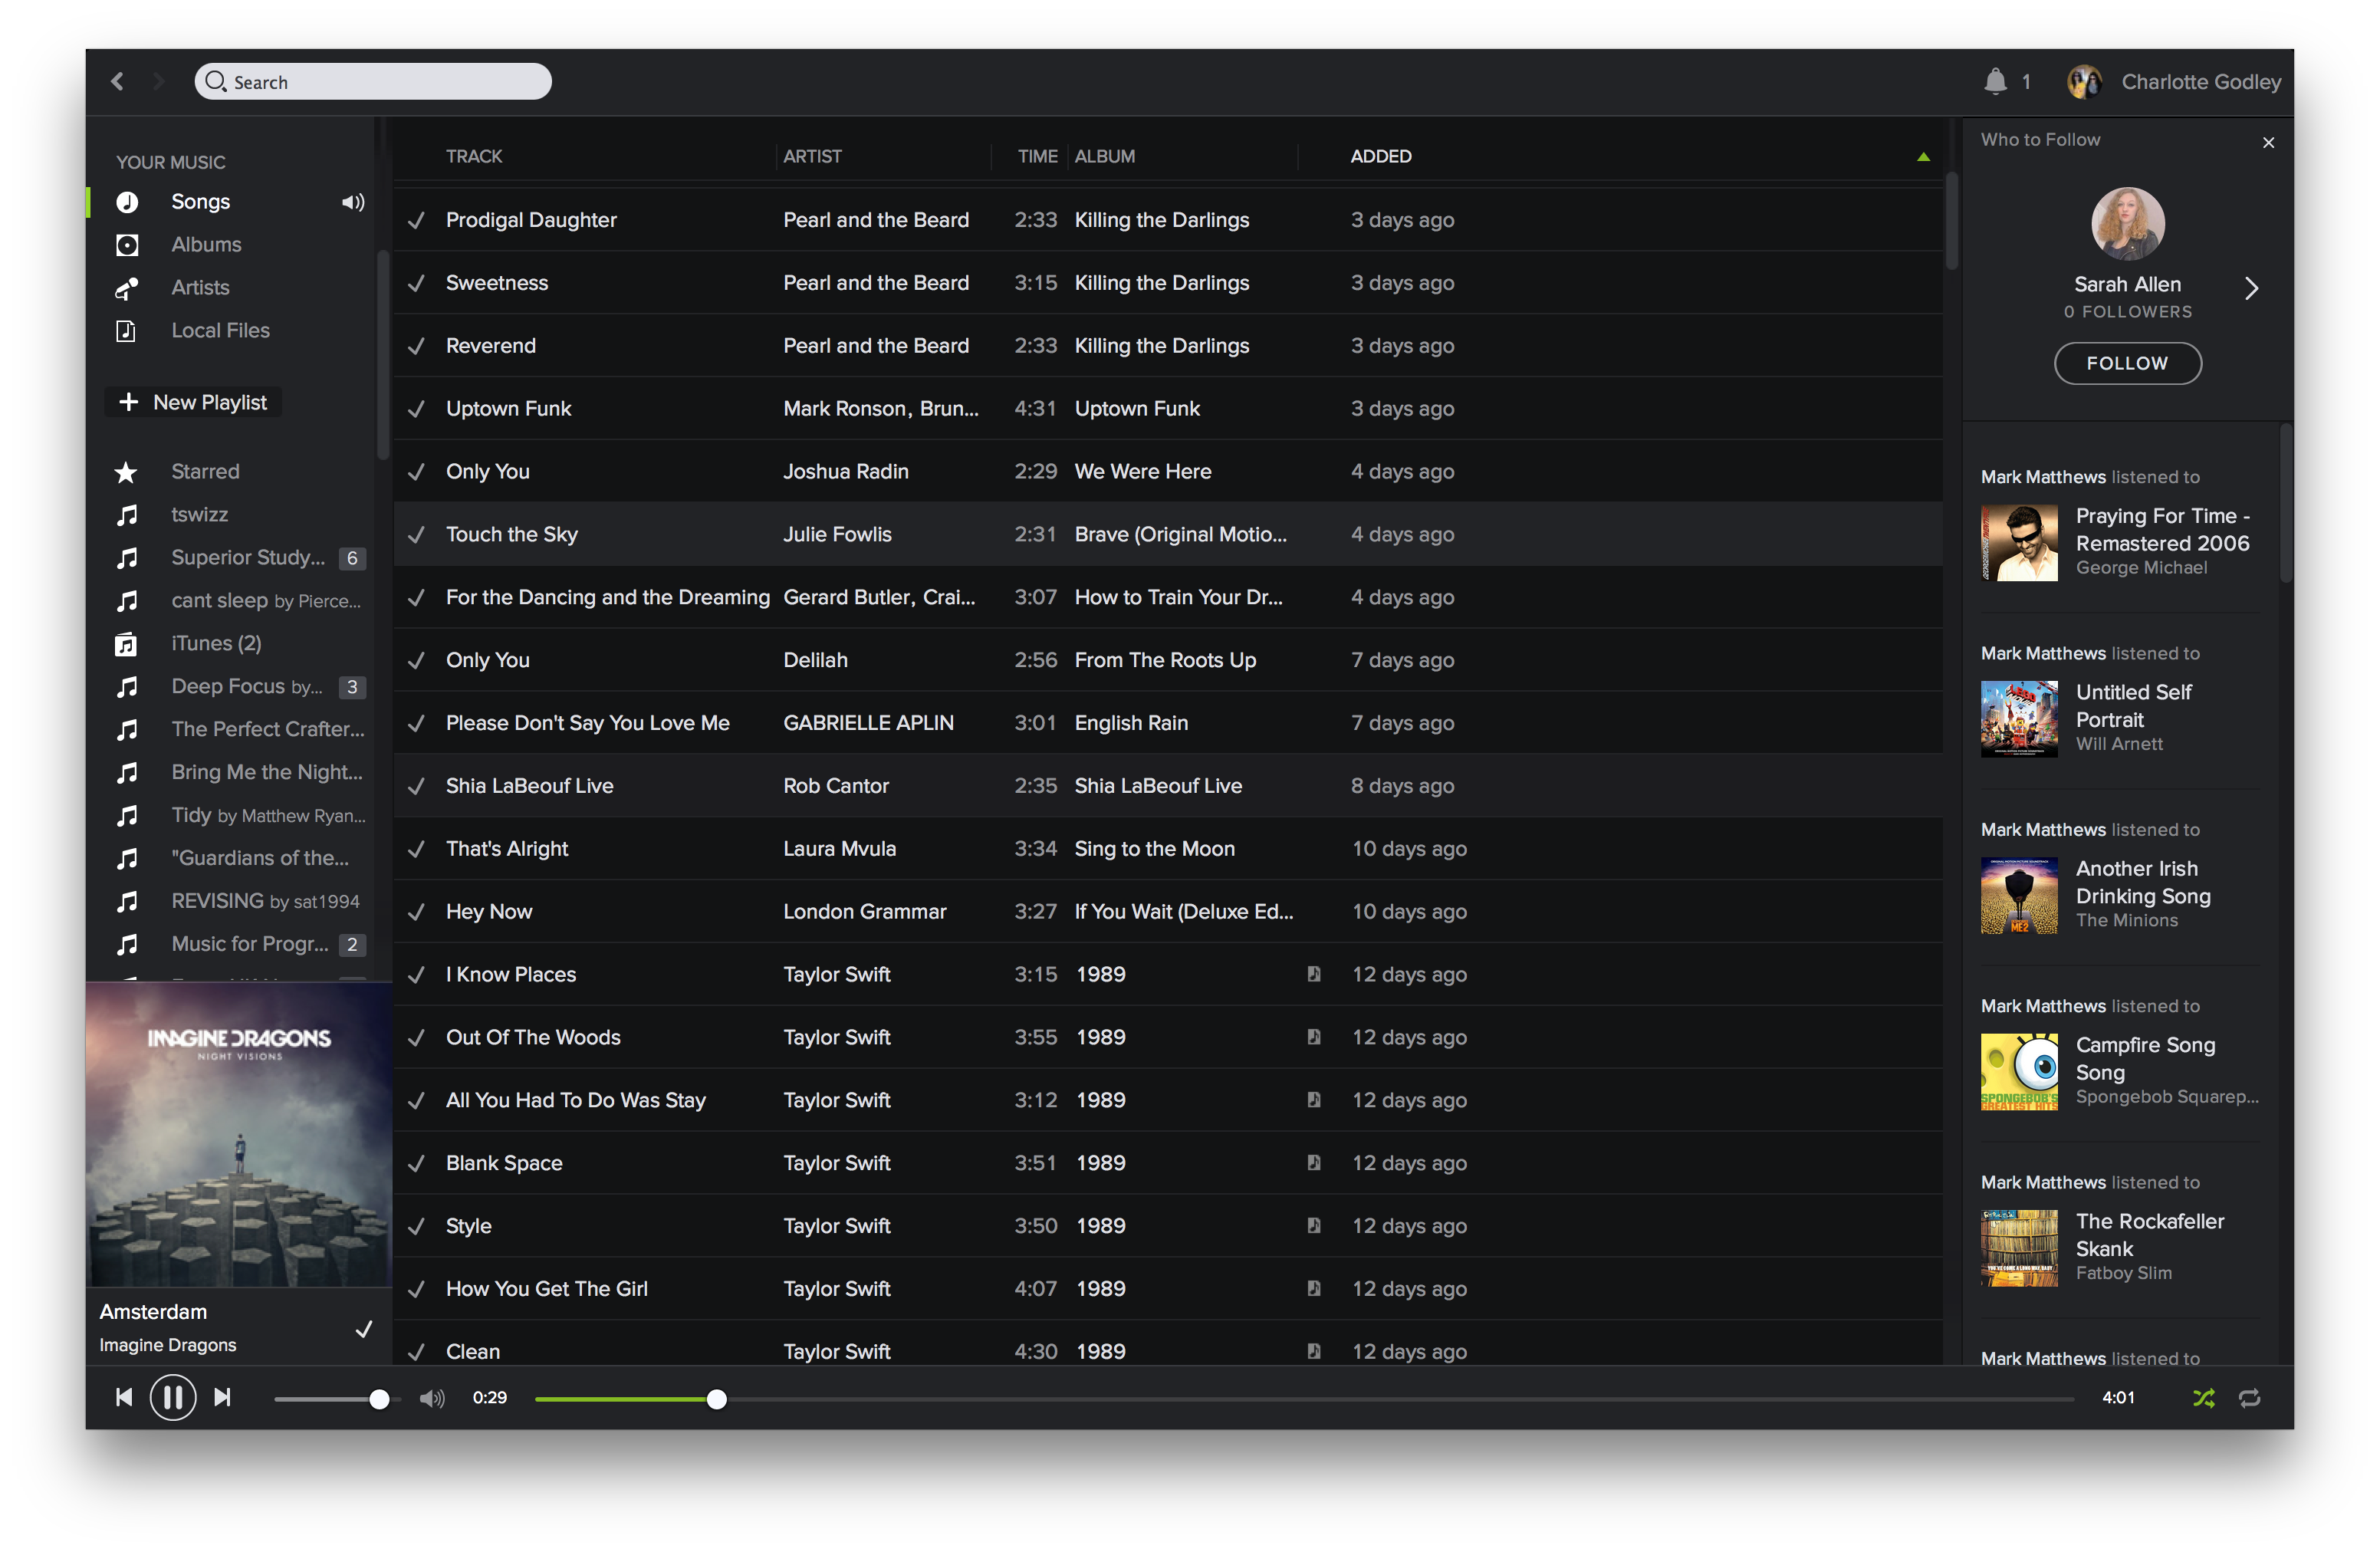
\includegraphics[width=\textwidth]{screen.png}
    \caption{Spotify user interface}
    \label{fig:spotify}
\end{figure}
\subsubsection{Main Display}
\begin{figure}[H]
	\centering
    \includegraphics[width=500pt]{main_diagram-crop}
    \caption{Main User interface of the project - design}
    \label{fig:main}
\end{figure}
Figure \ref{fig:main} shows the main view of the application, as mocked up before being developed and implemented. The developer took the this design, and the others which are in the appendix and produced a prototype using QtDesigner. This prototype is shown in figure \ref{fig:annotated}, updated to show details about the sheet music displayed in the PDF window.
\begin{figure}[H]
	\centering
    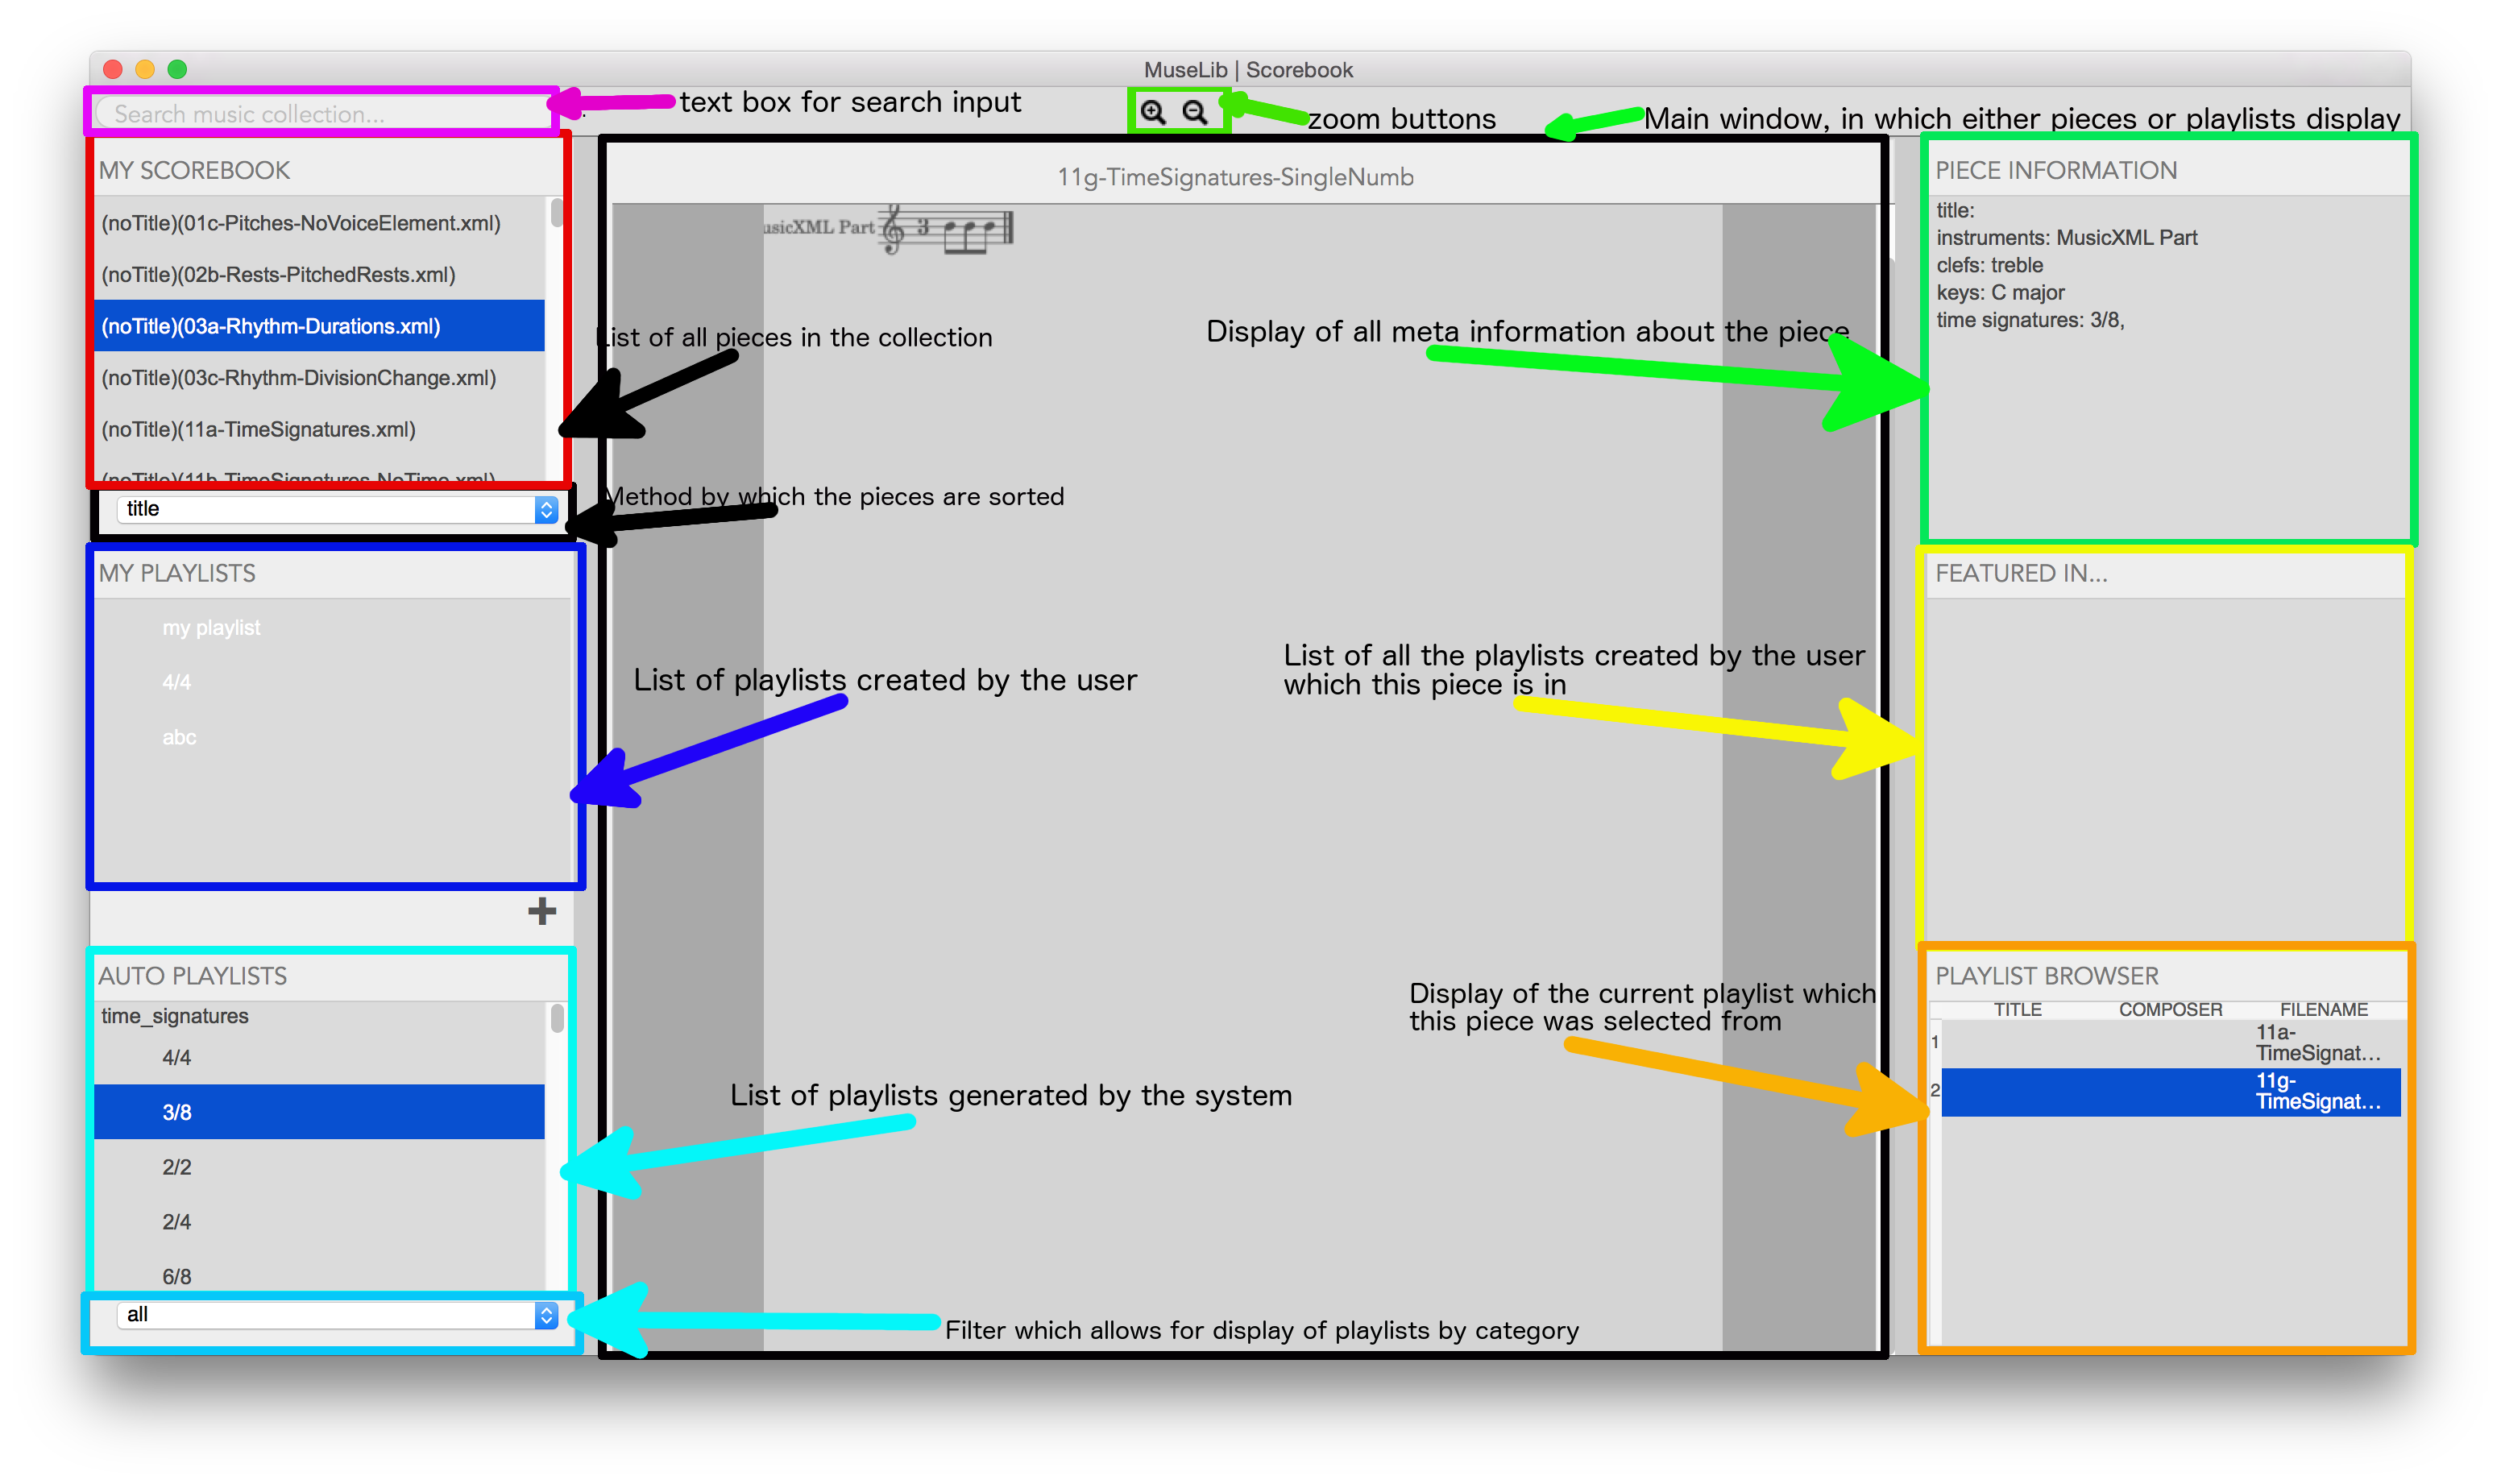
\includegraphics[width=500pt]{annotated_gui}
    \caption{Main User interface of the project - implementation}
    \label{fig:annotated}
\end{figure}
All of the frames of the user interface are styled using a CSS stylesheet, so that the developer could customise everything with precision. The use of CSS also enabled the developer to easily create new themes. The remaining screenshots with an explanation of how different windows link together and screenshots of the additional themes are given in the user guide which is in the appendix.

\subsection{Test Design and System Testing}
\subsubsection{Test Driven Development}
The project was developed using Test Driven Development (TDD). Test Driven Development is an Agile software development methodology which utilises the rule that a line of code should not be written unless there is a failing automated test \parencite{TDD}. This methodology has been chosen because the nature of the notation of music means that attention must be paid to how and with what symbol every element is notated, and Test Driven Development will significantly improve the quality of the software by closely integrating testing with the development process.

As such, the test plan is the same as the feature list provided in the appendix, as tests were developed at the point of introducing each new feature. Each class and file containing tests was designed to be a self contained unit testing the smallest possible details, such as an accent being added to a measure correctly, or a note's pitch being created with a particular note name or octave number.

\subsubsection{Unit Testing}
Unit tests for this project were created on an objective by objective basis using the standard python unit tests testing suite. The developer's IDE of choice, Pycharm, has built in support for this module, with an intuitive interface for running tests in a given file and production of readable output of what happened in each tests, as shown in figure \ref{fig:testing_interface}.

\begin{figure}[h]
	\centering
	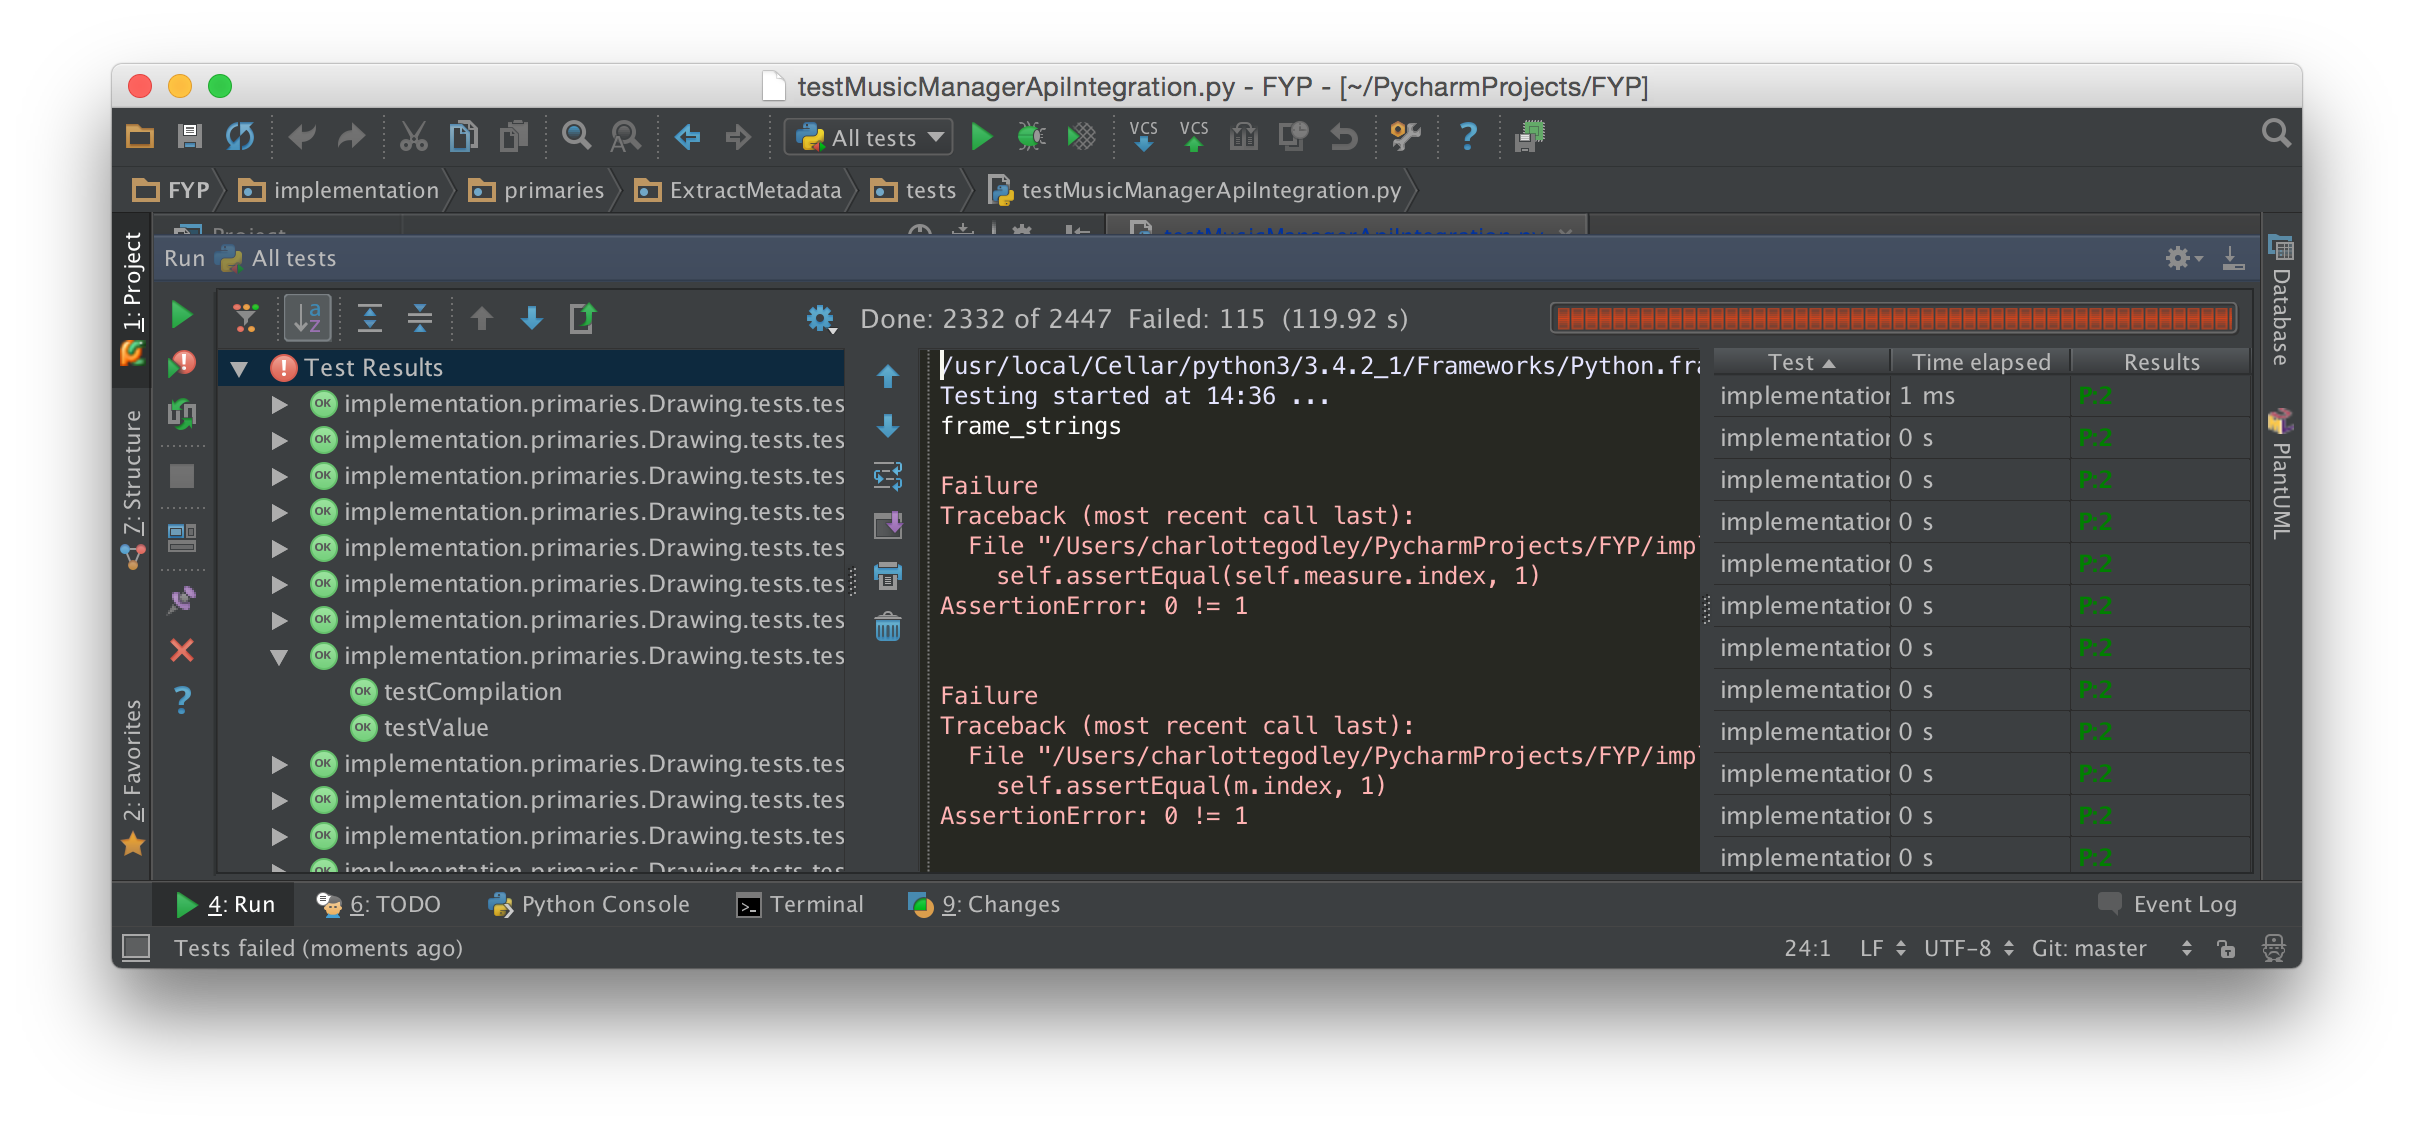
\includegraphics[width=\textwidth]{testing_interface}	
	\caption{An example of testing integration in PyCharm}
	\label{fig:testing_interface}
\end{figure}

The interface also includes the ability to create scripts which discover and run tests on folder, file, class and method level, as shown in figure \ref{fig:testscript}. The developer used this feature to create scripts which ran all of the tests for specific areas of each objective, as well as the objective itself. This enabled the developer to quickly check new features had not affected the status of previous features. 
\begin{figure}[H]
	\centering
	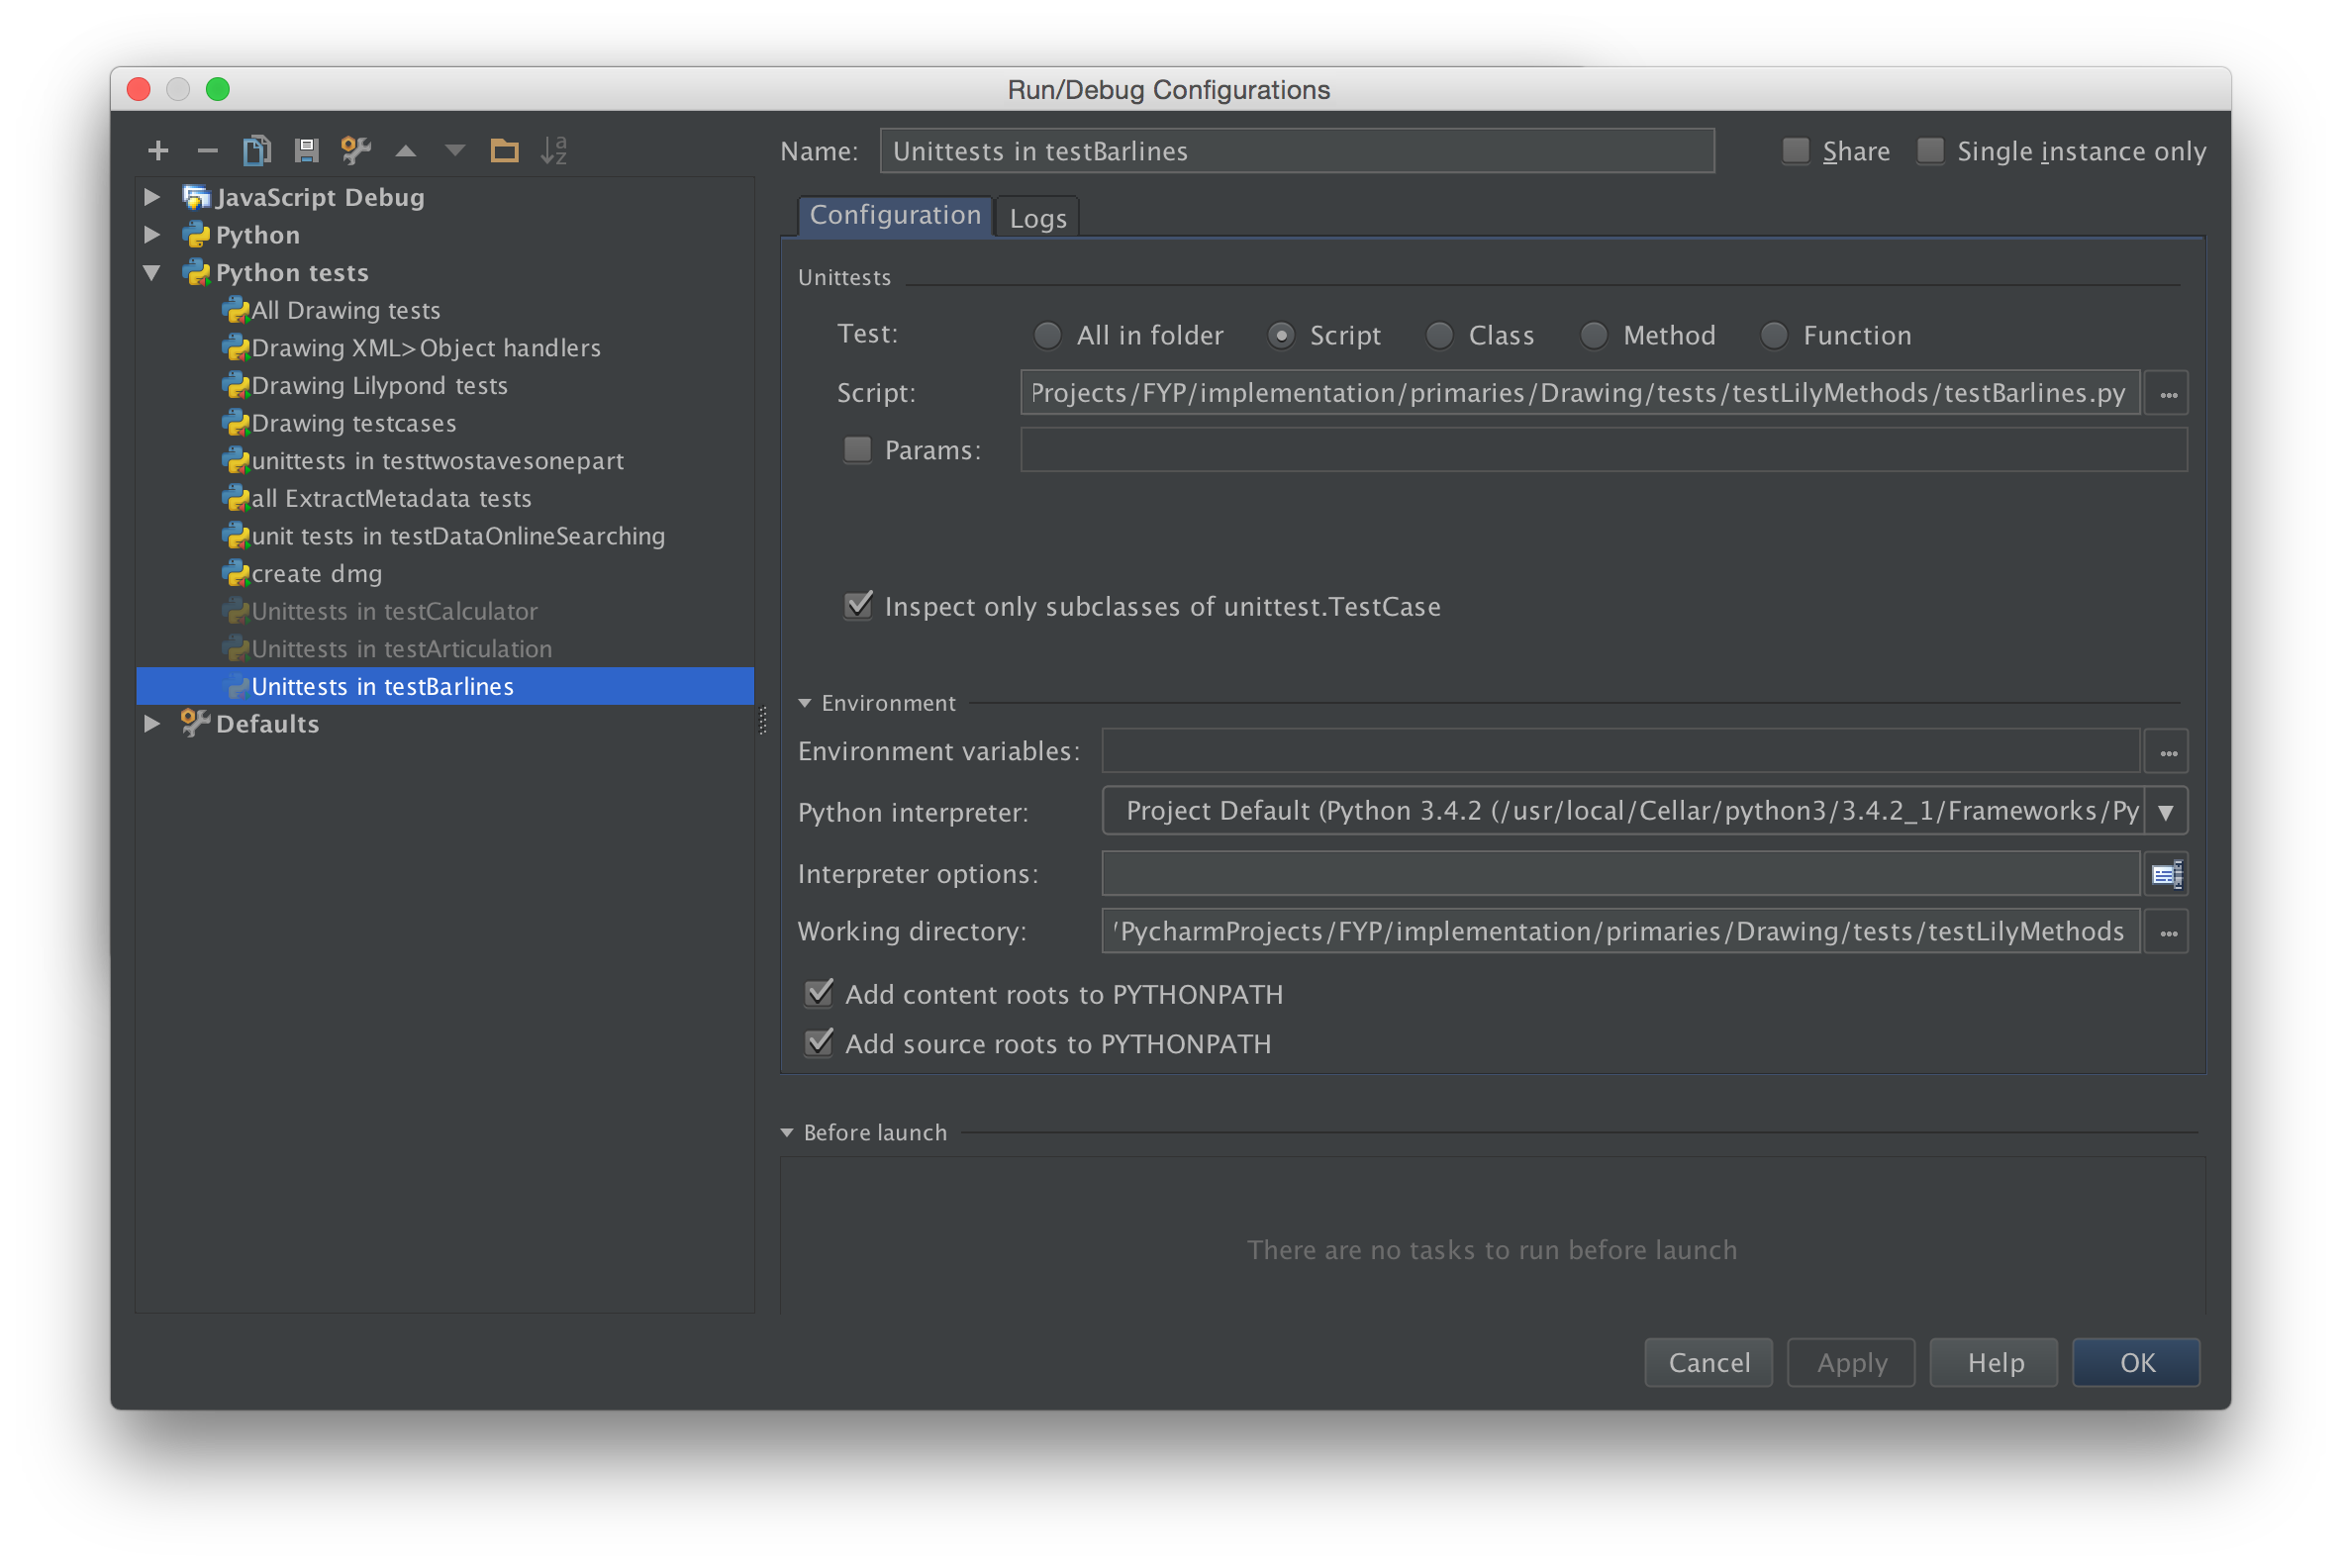
\includegraphics[width=400pt]{create_test_script}	
	\caption{An example of script creation in PyCharm}
	\label{fig:testscript}
\end{figure}
\subsubsection{Unit Testing the rendering system}
In the initial phase of developing the rendering system, the SAX parser was tested at base functionality level, with checks that new tags, new data and closing tags modified various lists which handler methods used to extract information. As new functions and tags were handled, more and more tests were developed for every tag, termed handler tests. These tests included combinations of tags and combinations of tag attributes, as well as testing tags in exclusion from other tags. When new features were introduced the developer would run the full set of unit tests before committing the code to source control, in order to ensure that new features did not cause regressions or changes in previously developed code.

When the object extraction algorithm portion of the rendering system was completed, the developer created unit tests for the individual symbol classes to confirm their ToLily method worked according to what was expected in the Lilypond documentation. 


Once the individual symbols were tested, the developer created tests to check the classes containing the symbols concatenated the strings of output in the correct order. As every possible value and change to each symbol had been tested at symbol class level, this portion of testing was not as extensive and only included tests to confirm ordering of notes, directions and expressions were valid where they had any effect on each other. For example, it would be unnecessary to test a note with every possible dynamic marking, but it was necessary to test a dynamic did not occur before a note.


\subsubsection{Development of Test cases}
In order to test the system more extensively, the developer created several MusicXML test cases. A full list of the test cases used is given in the appendix, as well as a sample file. In order to produce the test cases the developer used the composition software MuseScore, and systematically went through each category of symbols provided producing every possible type of symbol for that category. These were saved as individual files, titled by each category of symbol.
The developer then produced unit tests which checked the object hierarcy when the parser loaded the file. Each test and test method confirmed that the objects were in the right place within the piece, part and measure, and that each object had the appropriate values.

Once the lilypond output section of the objective was completed, the developer reused the test cases to check their lilypond output. Initially, the tests were primitive, only confirming that a pdf file with the same name had been created. Later, the developer produced an expected output lilypond file and checked the output of the test against the expected output.

\subsubsection{Use of Third Party Test cases}
As there was no official test suite available for MusicXML, the Lilypond project released an unofficial collection of music xml files for testing purposes \parencite{LilypondTestcase}. Each file tests individual elements of music xml, sometimes in collaboration with other areas. In total the test suite contains 131 files and represents the most comprehensive test suite currently available openly.

The developer ran the rendering system against each test case in the suite. Initially, the developer ran them individually, visually checking the output against the images in the documentation for the test suite, and then moving test cases which passed to a separate folder from the remaining test cases. Later, an automated script was created to attempt to speed up the process, though visual checking of the output was still necessary as no lilypond files were provided with the xml files.


Due to time constraints, the developer prioritised failures according to severity, which had three levels. The first level was failure to produce a lilypond output due to an exception in the program. The second level was failure to produce a pdf output due to the lilypond output being invalid. The third and final level was failure to produce a pdf output which matched the expected output. Each failure in any sense was reported using the issue tracker on Github, with an indication of the filename which failed as well as the reason for the failure. An example of such an issue report is given in figure \ref{fig:issue}.

The developer ensured that all test cases were above the first two levels of severity, and then made a decision on how important the symbol was in the context of it's usage in western music, as well as the time remaining to work on the other two primary objectives.

At the point of stopping work on the rendering system, 65$\%$ of the test cases in this suite passed and produced the correct graphical output. 
\begin{figure}[H]
	\centering
	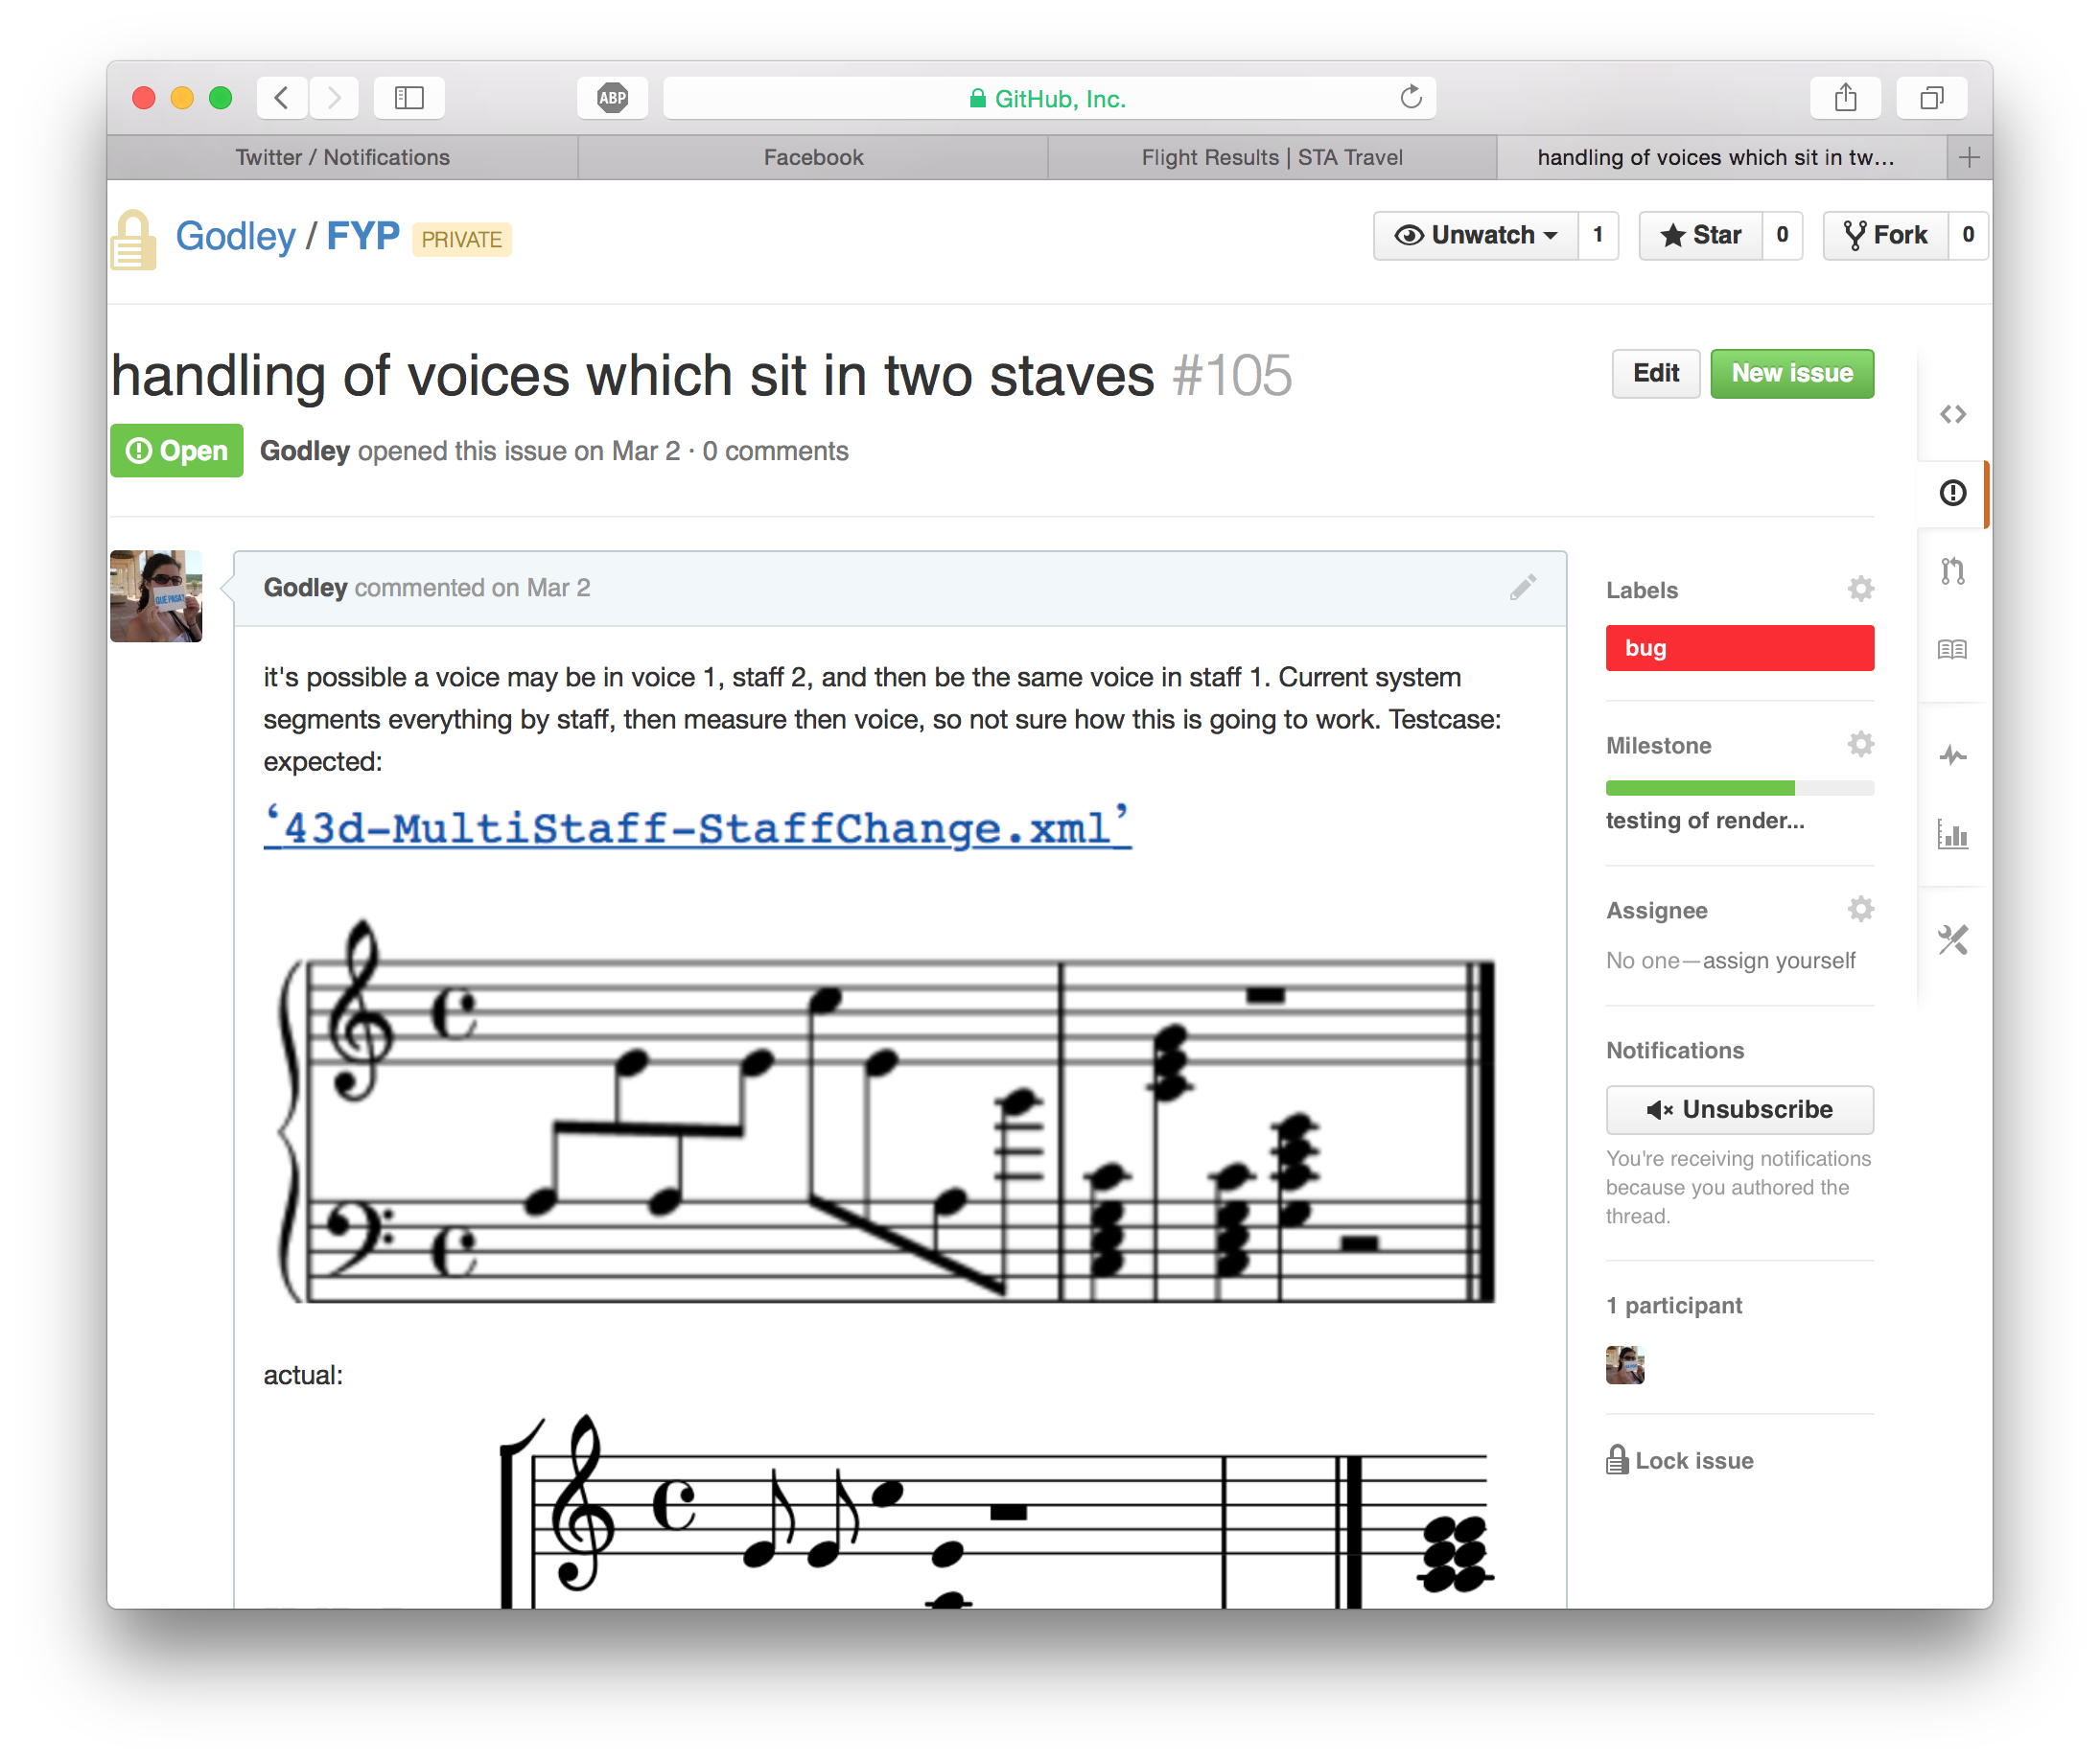
\includegraphics[width=400pt]{issue_report}	
	\caption{An example issue report}
	\label{fig:issue}
\end{figure}

\subsubsection{Unit testing the metadata and API objectives}
Unit tests were written for the other two objectives in a similar way to the rendering system.

For the metadata scanning objective, the developer tested each element of the system in exclusion from each other. This divided the process into four classes, the folder browser, the unzipper, the data layer, and the metadata parser, as visualised in the class diagram in figure \ref{fig:metadiagram}. One main class, the music manager, handles the connections between each element. Like the rendering system, this meant that the tests for combining the elements together did not need to be so complicated as the functionality of each element had been tested rigourously.

For the online collections objective, tests were created at source API class level, then API manager level, and finally the API manager was tested when integrated with the music manager class.

\subsection{System Design}
\subsubsection{Overall Architecture}
The flow chart in figure \ref{fig:flowchart} was designed in the initial prototype phase in order to visualise how the objectives would interlink with each other.
\begin{figure}[h]
    \centering
    \includegraphics[width=400pt]{diagrams/overall_system.pdf}
    \caption{A flow diagram describing the project}
    \label{fig:flowchart}
\end{figure}

\subsubsection{Metadata Scanning system}
The flow diagram in \ref{fig:flowchart} refers to applying a metadata scanning system to the folder. This is described in more detail in the flow diagram in figure \ref{fig:meta}. 
\begin{figure}[H]
    \centering
    \includegraphics[width=250pt]{metadata_algorithm-crop}
    \caption{A flow diagram describing the meta scanning system}
    \label{fig:meta}
\end{figure}
\subsubsection{Metadata Class Structure}
The metadata scanning objective implements the popular Model View Controller design pattern, which separates the user interface (view) from the program logic (controller) and any databases or information storage (model) \parencite{mvc}.
In this instance, as shown in the class diagram in figure \ref{fig:metadiagram}, the music manager class acts as the controller, which takes input from the application interface. The music manager processes the input and turns it into requests for data, which are sent to the data layer. The data layer communicates with an SQLite file containing several tables, and sends collections of requested data back to the music manager, which updates the user interface with the new information.

The decision was taken to use this pattern in order to avoid coupling to any particular database and to ensure that the objective was properly organised according to functionality. The decision was also influenced by considerations about the future of the project, including expansions to include online data layers or improvements to the UI without affecting program logic.

\begin{figure}[H]
    \centering
    \includegraphics[width=\textwidth]{diagrams/api_and_meta_data_diagram}
    \caption{Metadata and API Class Diagram}
    \label{fig:metadiagram}
\end{figure}

\subsubsection{Modular Design}
The MVC design pattern was complemented by the implementation of the  modular design pattern, in which functions and collections of functions are separated into independent blocks or modules \parencite{modular}.

This is shown in the class diagram in figure \ref{fig:metadiagram} as the music manager also interacts with other classes such as the folder browser, which handles all functionality involving scanning the given folder for new, old, or zipped files, and the unzipper, which handles the functionality for manipulating zip files.

It is also present in the rendering system explained in detail in section 4.3.5, as each section of the object hierarchy collects its own Lilypond formatting, and then calls upon its child classes to collect theirs, finally collaborating into one complete Lilypond file. In the context of sheet music this is particularly important, as symbolic notation has many options for symbols which may or may not be present, so in program logic they must all act independently of other symbols occurring in the file.

This design was influenced by the decision to use test driven development, as this development methodology aims to test small units of program functionality in an isolated environment \parencite{TDD}.
 As such, this was easier to achieve if each independent class had one role in the system, with management classes handling the collaboration of these roles without needing to test multiple elements of functionality at once. 

This makes the code and overall architecture reusable in different situations. For example, the API manager class sends data collected online back to the Music Manager, which can then communicate with the metadata scanner to extract further information, which avoids code duplication.

\subsubsection{Rendering Architecture}
The class diagram in figure \ref{fig:classdiagram} shows an abstract structure of the sheet music rendering implementation used in this project. This implements a tree, each node of which holds an item containing the notation specific to that node. Each node object implements the ToLily method, which generates a string of Lilypond formatted output representing itself and then calls each of its child nodes in turn for their outputs, combining them into one string. 

A tree was chosen as the object structure in order to give an indication of time, and in order that specific elements could be positioned according to sequential instructions from the MusicXML parser. 

Each node in the tree inherits from the Node class. This class gives some generic methods for manipulating and returning its children, which each of the sub classes use in their own specific manipulation methods. Node is different from IndexedNode only in the sense that node contains a list of children, whilst IndexedNode stores them as a dictionary. The indexed node is used in the Staff, Voice, Measure, Part and Piece nodes because each of these classes contains items which have specified keys when they are loaded in using MusicXML, but anything below the voice node does not have an index in MusicXML.

Symbolic classes which add elements to a note or to a measure are added using the methods supplied by measure which contains the logic to decide what to do with the element. The measure handles additions, rather than the note to which the element should be assigned, as some elements must wrap the measure in Lilypond code, some must wrap a note and other more simpler elements add their code to the end of the current measure or note. The logic to decide what to do with the element is easier to achieve at measure level rather than note or direction level so that all options are available.
\begin{figure}[H]
    \centering
    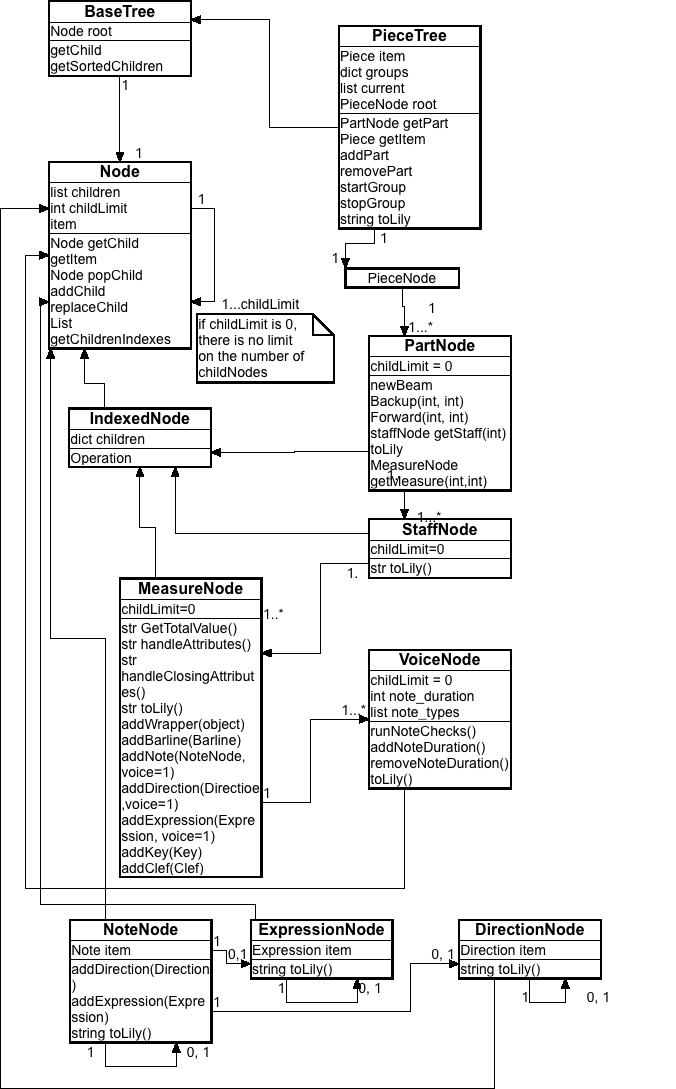
\includegraphics[width=250pt]{diagrams/render-tree.png}
    \caption{Renderer Class Diagram}
    \label{fig:classdiagram}
\end{figure}




\subsubsection{Duck Typing}
The rendering system visualised by figure \ref{fig:classdiagram} implements a feature of dynamic typing known colloquially as Duck Typing. Duck Typing is a method of type inference by which the program assumes that an object is of one type according to the behaviours that it has, not the exact type or attributes it may or may not contain. %todo ref

In respect to the rendering system, duck typing is applied in the production of output, whereby each class assumes any child classes present will have the ToLily method, call the method and concatenate the results. Using this method of type inference is important to the project as this avoids assumptions about what the music will or will not contain, and instead defines that symbol as suitable for inclusion if it has the ToLily method. Using type inference means that future symbol classes which are implemented only need to provide a ToLily method and be linked into the MusicXML parser in order to be included in the output.

Duck typing can have some negative effects in system design and development. For example, if a class does not have that method this could cause the program to crash without warning. Static type checking used by other languages such as C\# and Java would avoid this problem and create a more robust program. However, the use of test driven development and the generation of test cases have counteracted this risk sufficiently to make the design decision worth taken, resulting in a fluid, experimental and rapid development environment.

\subsubsection{Designing for extensibility}
The project is designed with a particular aim of extensibility. This affects each area of the system in a different way, but in general, it means that the elements in the system are able to be modified, improved or expanded without requiring changes to the organisation of the system. 

An example of this is the API manager, which holds a dictionary of sources, with each index pointing to a class. The API manager will cycle through these sources when its methods are called, meaning that to implement a new API, the developer would simply put a new entry into this dictionary.

Each source implements the API class. To avoid causing problems with classes missing particular methods, the API class will throw a not implemented exception if the sub class does not override the method, in order to indicate to the developer working with a new API that this method is necessary.

\subsubsection{Difficulty Rating input from users}
When considering the difficulty rating objective for this project, the developer was aware of the subjective nature of sight reading and rating. To assess how this varied from instrument to instrument, the developer produced a survey which was given to a wide range of musicians, as shown in figure \ref{fig:survey_difficulty}. The results of this survey are given in the appendix.

\begin{figure}[H]
\centering
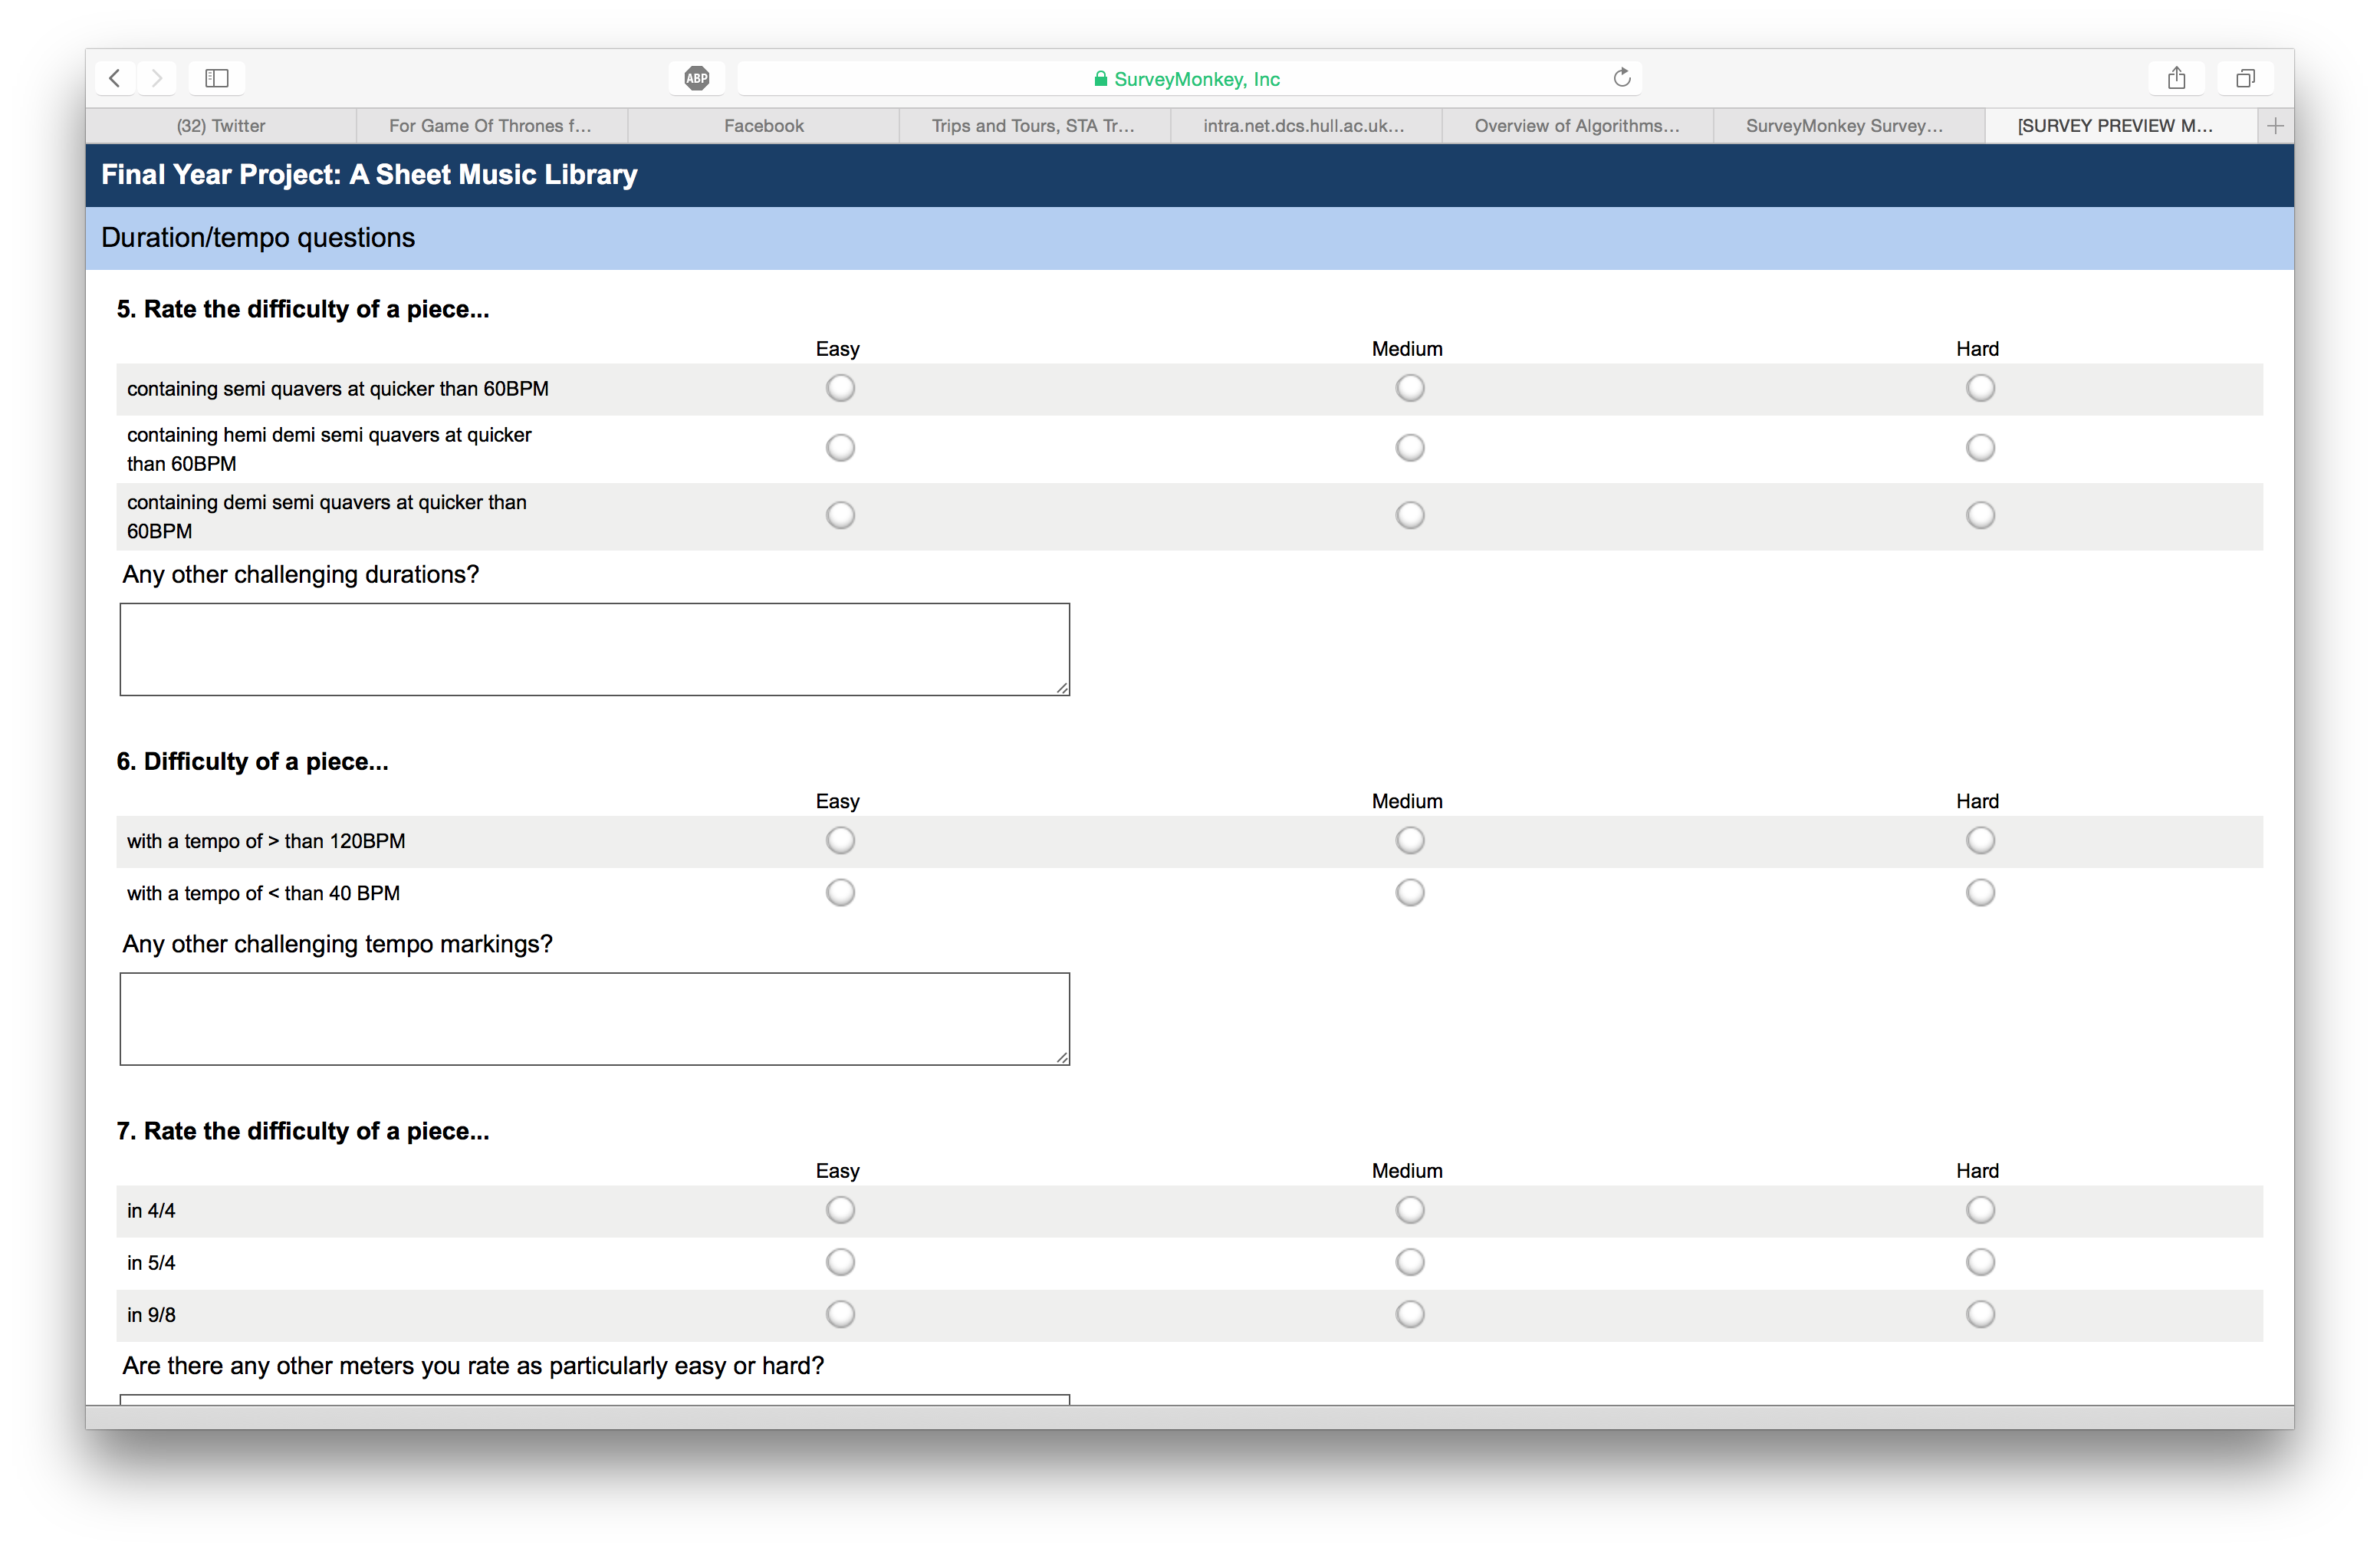
\includegraphics[width=400pt]{survey_difficulty}
\caption{An online survey on piece difficulty}
\label{fig:survey_difficulty}	
\end{figure}



\subsection{System Implementation}
\subsubsection{Development Methodology}
The project was implemented using a developer informed process. In this process, the developer would review the project's status for bugs, issues and features which had yet to be implemented and note this using the Github Issue Tracker. When the developer began working with the code, they would select an issue based on the priorities of the project, develop tests for this issue and finally, develop the production code and close the issue.


Issue tracking and reporting was used so that the developer could think and reflect on areas of the system which needed improvement, modification or implementation. The methodology worked well in the context of a year long project in which development was not continuous because it ensured that when development was paused, the developer could see instantly what needed to be doing or what was being worked on before the pause to work on something else. 

This adds the benefit that in the future, when this project may be worked upon by more than one developer, new developers can see things which have yet to be implemented and choose which features are most relevant or doable by their own standards, as well as discuss or contest previous issues in the system.


\subsubsection{Challenges in the rendering system}
The renderer in this project was designed around two open formats - MusicXML and Lilypond. Whilst every effort was made to avoid coupling with either format, designing the system to work seamlessly with both formats was difficult, and many problems were encountered structuring the object format.

Initially, the project used a simpler object structure in which measures contained a list of items contained within that measure. The decision was taken to use lists of items loaded sequentially because elements belonging to each measure in MusicXML have no unique identifiers which could be used to indicate at which point they occurred within that measure, so objects had to be loaded and stored sequentially. An example is given in listing \ref{code:example}, with the visual representation given in figure \ref{fig:lilyexample}.
\lstset{
    language=xml,
    tabsize=3,
    %frame=lines,
    caption=Note followed by dynamic followed by note followed by dynamic,
    label=code:example,
    frame=shadowbox,
    rulesepcolor=\color{gray},
    xleftmargin=20pt,
    framexleftmargin=15pt,
    keywordstyle=\color{blue}\bf,
    commentstyle=\color{OliveGreen},
    stringstyle=\color{red},
    numbers=left,
    numberstyle=\tiny,
    numbersep=5pt,
    breaklines=true,
    showstringspaces=false,
    basicstyle=\footnotesize,
    emph={food,name,price},emphstyle={\color{magenta}}}
    \lstinputlisting{example.xml}
    
\begin{figure}[H]
\centering
\includegraphics{lilyexample-crop}
\caption{Example as represented in sheet music}
\label{fig:lilyexample}	
\end{figure}


It was then discovered that Lilypond dictates that dynamics and some other elements had to occur directly after the note to which they should be assigned \parencite{ExpressionLilypond}.  The above listing would look like figure \ref{code:lily} in Lilypond.

\begin{figure}[H]
\centering
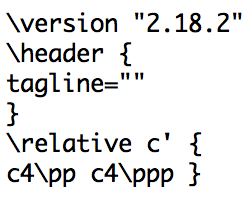
\includegraphics{lilyexample-code}
\caption{MusicXML example written in Lilypond}
\label{code:lily}	
\end{figure}


 The system was affected because some musicXML files, such as the one given in listing \ref{code:example}, contain directions before a note has occurred within the measure, which would cause the Lilypond output to be invalid. 
 The structure had to be redesigned based on this information in order to classify notes as first class objects, for which other elements would be indexed according to which note they occurred after. Directions and expressions needed to be split into two lists, in order to ensure that expressions (like dynamics) could be put before directions, but not before the note they should be assigned to.

Later it was discovered that MusicXML allows for navigation through a measure using two specific tags called "forward" and "backup" \parencite{forward}, which in the original system would require a lot of list manipulation to position elements correctly. 

Various other feature inclusions led to the developer redesigning the system around these factors, finally reaching the tree structure described in the design section. This enabled the developer to move objects around according to the tags which next occurred.

Fundamentally, the difference in the design aims for MusicXML and Lilypond is that MusicXML dictates a sheet music file by how it appears, as in the above example, sequentially positioning the elements is how a viewer would see the overall piece. Lilypond, on the other hand, dictates a sheet music file by how it is played - after all, a dynamic without a note would not achieve the desired result as these dictate the volume of a particular element or elements of music. 

 The change in design of the system was caused by the developer analysing a limited subset of cases for both the input file format and the output format. It may have been a suggestion to extend the research period before development to accommodate this, but a research period long enough to understand the design aims of the formats in enough detail to fully design the structure from the outset would have reduced the development time by a significant amount. Redesigns and refactors were made at late stages of development, and new data structures were considered to solve the problem. The options were analysed according to their various merits in recursive sorting and searching, as well as the links which needed to be made between each symbol or element of music. The late redesign and refactor was implemented after a period of experimentation with new data structures, where a generic tree structure was assessed against a linked list. The test harness highlighted areas which the developer needed to change in order to have a working refactored system. This improved the quality of software and reduced the development time needed to find and fix problems.
 
 However, the negative side of having a test harness so extensive was that changes to production code sometimes required changes to test code, depending on the assumptions of the previous system design. Each test which failed had to be reviewed first for whether it failed because of these assumptions, or whether it was a genuine bug in the production code. Despite this negative aspect, the developer regarded the test harness as a benefit which improved the quality of the software and ensured no detail was missed. 
 
\subsubsection{Use of external technologies and libraries}
For this project, external libraries were used for the graphical user interface and for the database layer. Both were necessary to avoid development duplication and will be discussed in the sections below.

\textbf{User interface libraries} \\
There are several libraries available for creating a graphical user interface in Python, with the most popular ones summarised in table \ref{table:gui}.

\begin{table}[h]
\centering
\begin{tabu} to 1.05\textwidth {| X[c] | X[c] | X[c] | X[c] |} \hline
  {\textbf{Library}} & {\textbf{Benefits}} & {\textbf{Drawbacks}} & {\textbf{Cross platform}} \\ \hline
  Qt & Has its own designer program (QtDesigner) and some other third party designer programs & Long installation process & \checkmark \\
  & & no built in PDF viewer & \\
   &  popular amongst many languages &  & \\
   & & & \\
   &  can use CSS to style widgets & & \\\hline
  Wx 
  & Built in PDF display & Designers not as powerful as Qt + all are third party & \checkmark \\ 
  & several designers made for it &  & \\ \hline
  TKinter & Built into Python itself & No designers & \checkmark \\ 
  & & No built in PDF/PNG viewers & \\
  & & Binds to an old language which is rarely updated &  \\ \hline
  AppKit & Works well on OSX & OSX only &  $\times$ \\ \hline
  
\end{tabu}
\caption{Table of GUI libraries in python}
\label{table:gui}
\end{table}

In Python there is only one library in popular usage (AppKit) which is locked to one platform, as shown by the table. This library was ignored due to it being locked to one platform.

In the initial phases of GUI prototyping, the developer trialled two of the suggested GUI libraries.


The first trial was TKinter, being as it is built into the Python library and did not require any further installation. TKinter is a library which provides a python binding to TCL's user interface libraries \parencite{PythonTCL}.
 The TCL user interface library has not been updated or upgraded for today's image formats, and does not support PDF or PNGs. Any use of either of these formats required installation of other libraries, such as the Python Image Library (PIL) \parencite{PIL}.
 Furthermore, as discussed by \cite{GuiProgramming}, there are very few open, non-commercial options for graphical GUI designers for TKinter, meaning that any interfaces had to be hard coded using python code, rather than creating designed files to be imported.
 
 
 The second trial was Qt. This library took longer to install, being as PyQt, like TKinter, is only a binding to a lower level C++ library. This means that PyQt cannot be installed in the same way as Wx, using the Python Package Library pip, and for windows meant installing and compiling all sections of PyQt, Qt and SIP which links the two together from source, as no pre compiled installer was available.
 
 In addition to this development time, Qt does not provide a widget for PDF documents, which meant the developer installed a second third party library called Poppler, which is also a C++ library with Python bindings. This library was found to be far easier to use than the Python Image Library used by TKinter.
 
 Whilst this extended the time taken to produce a fully cross platform application installer, Qt provides a fully extensible QtDesigner application, which enables developers to produce their designs, including applying CSS to widgets, in a graphical user interface which outputs UI xml files. 
 
 The xml files are then loaded into Python, meaning that any changes to the files through the designer automatically affect the python binding the next time the developer runs the application.

Furthermore, as Qt is a common library to other languages and is reasonably popular, far more support was found for installing, using and extending Qt than the other libraries the developer tried to use, so the developer decided to use Qt.

Wx was not trialled because the developer felt comfortable using Qt for the reasons given above, and did not want to reduce development time further by trying a new library when Qt functioned as needed.

\textbf{Databases and Database Libraries}\\
Table \ref{table:databases} shows the options for databases the developer could have implemented in this project. These three options were selected because all of them are free and have a reasonable amount of documentation for beginners in each database.

\begin{table}[H]
\centering
\begin{tabular}{| l | l | l |} \hline
  {Database} & {Benefits} & {Drawbacks} \\ \hline
  MySQL & Open source & Installation process long \\
  & Widely used/supported & \\ \hline
  MongoDB & JSON friendly & Low developer experience with NoSQL \\ 
  & scalable & \\ \hline
  SQLite & Single file & some types not supported \\
  & Portable & not very scalable \\
  & Library built into Python & \\ \hline
  
  
\end{tabular}
\caption{Table of database solutions}
\label{table:databases}
\end{table}

The first option, MySQL, was dismissed because this application is not an online solution, and as such, the developer would need to install MySQL and probably have the user install MySQL on their machine when the application was created \parencite{mysql}. MySQL is also a much larger system which is not as suited to a smaller local application.

The second option, MongoDB was dismissed because the developer did not have experience with using NoSQL, the query language used by MongoDB. Furthermore, the recommendations for MongoDB usage are when an application has large amounts of data and needs to scale \parencite{mongod}. It is not expected that there will be a large amount of data when this application is in general usage, or that scalability is a factor unless future extensions use bigger data sets.

The third and final option, SQLite, was selected because of it's portability as it only creates one file upon connection. The library for SQLite comes with Python itself and is fully documented in Python's documentation site \parencite{PythonSQLite}. The developer found the library intuitive to use which helped to reduce development time.


\section{Evaluation}
\subsection{Project Achievements}
All four primary objectives of this project have been implemented, and as such the project is considered a success. The four primary objectives of rendering sheet music, extracting data from the sheet music files provided, processing queries on the data collected and expanding the collection using online sources were set as each contribute a way to automatically organise, expand and view their collection and are achievable, measurable objectives. The sub sections below go into each objective in detail, in order to convey any particular technical challenges which had to be overcome to reach each objective.
\subsubsection{Rendering System}
This project implements the ability to view sheet music stored as MusicXML files. Composition software such as Finale by \cite{finale}, MuseScore by \cite{MuseTour}, and Sibelius by \cite{avid} each implement their own file format and provide export and import options to and from MusicXML. Focussing on their own file format means that the input and output of MusicXML is less precise, proven by the number of issues in the MuseScore issue tracker shown in figure \ref{fig:issues}.

\begin{figure}[H]
\centering
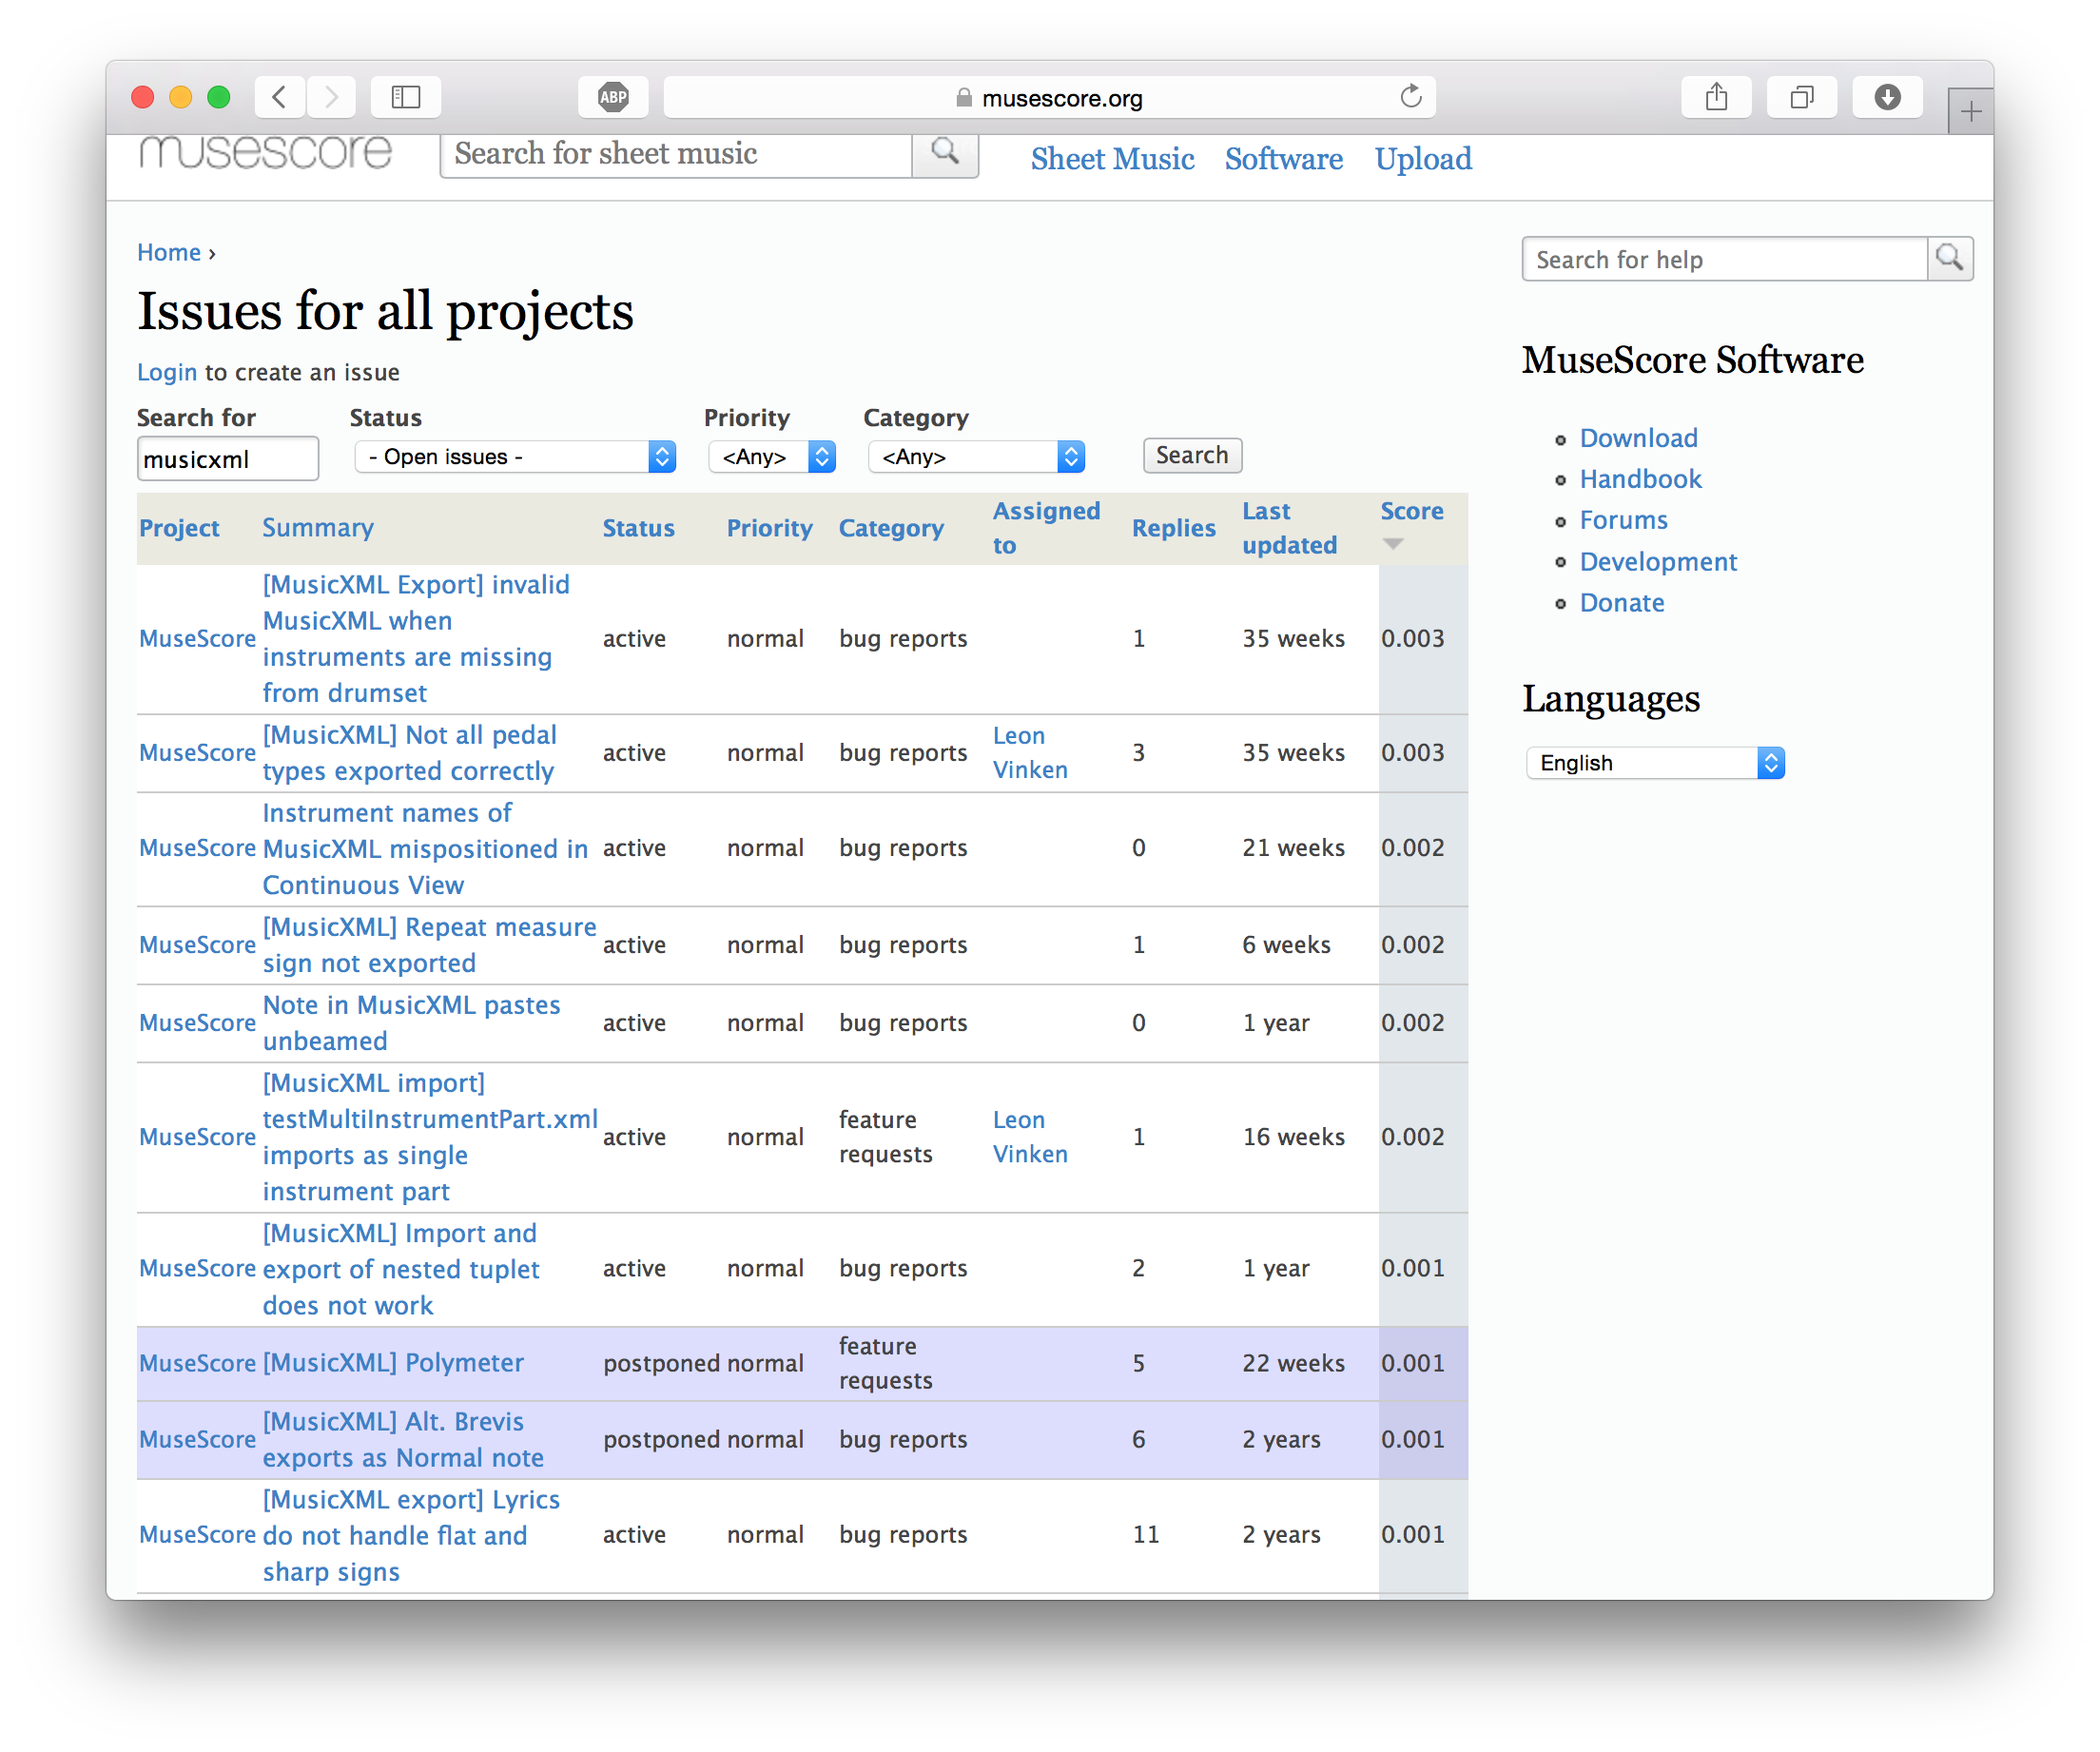
\includegraphics[width=400pt]{issue_tracker}
\caption{Issue tracker for the MuseScore project}
\label{fig:issues}	
\end{figure}

This project focussed on MusicXML, and therefore the input and output of elements should be more precise than the software referenced in the previous paragraph. This is achieved with low coupling to either format, as the system implements an object structure to manage communications of data into or out of the system.

Technical challenge was overcome in designing the objects used in the system around two separate input and output formats which had very different design aims for how sheet music should be stored and processed. This was achieved in the late stages of development through redesign with the test harness confirming that implementation of the redesign did not introduce any problems.

The classes and scripts for input and output are loosely coupling to other features, meaning that it would be possible for a new developer or new project to take this code and use it in a different context without requiring other objectives and features to make the system work. Using the SAX method of XML parsing means that the renderer can easily be extended and iteratively improved to handle more and more complex XML information.

\subsubsection{Metadata scanning}
This project implements the ability to organise sheet music through the extraction of information about each piece of sheet music. The information is general in the sense that the data collected is of relevance to the majority of pieces of music and all instruments. 

Further to automated scanning, the system allows users to create their own playlists. The search with suggestions system described in section 5.1.3 is modular, so the playlist creator has the same query structure and abilities as the general search function.

The metadata model created for this project was designed so that it would be of the most use to all performers. This design decision was made so that the application would be useful to a cross section of musicians, and with the additional intent of defining a standard model for future projects to implement.

\subsubsection{Search and Playlist operation}
From the extracted metadata it is be possible to search the catalog of music for specific requirements, such as key, clef, meter, time signature. This is achieved using a string of user input which is transformed into queries, which are handled by the data layer.

Suggestions for what the user might be looking for are updated in near-real time and avoid blocking the user from updating their query using multi processing. The challenge overcome here was designing the syntax for a non-technical user, but providing enough scope for complexity to produce a wide range of queries, and was achieved using a mix of language processing and new query syntax.

The system also uses the meta information to produce auto generated playlists which are listed in the user interface. Playlists provide an alternative viewing format to queries, in that it provides a list of pieces which are related to each other, and was made part of the search objective as this is a way in which the data can be used to create an organised user interface. 


\subsubsection{Importing Online APIs}
The application makes it possible to connect to online music collections and search them using the same user interface as searching for local files.

A general API class was implemented in this project to handle communications with networked sheet music collections. This class will be useful to future applications or extensions as new sheet music collections can easily wrap their own APIs in this class, and implement them without needing too many requests or changes at code level.

Whilst the API initially downloads an XML file in order to extract information for every piece in the source, when a user decides to download a file, the API will request PDF files where available. This means that the renderer does not have to be used, which reduces the processing overhead needed for downloaded files to be displayed.

Furthermore, applying the same model and metadata scanner used on local files to online files makes this feature more useful, as users can search their local collections and online collections using the same queries. This enables users to expand their collections without leaving the application or changing their behaviour.

\subsubsection{Cross Platform Capabilities}
All four of the objectives and the graphical user interface for this project are built to be used on the three most popular operating systems - Mac OSX, Windows 8.1, and Ubuntu (GNU/Linux).

A packaged version of this application has been produced for OSX, with work to produce a Windows installer program ongoing. This was achieved by paying close attention to which libraries were available in Python and avoiding any which did not explicitly state they would function cross platform.

\subsubsection{Graphical User Interface}
All of the objectives and functions of the program are accessed from the same user interface, which provides several views and options to the user depending on how they wish to view and organise their music. As well as automatic organisation, this also provides a create playlist function which allows users to create sub-collections of music which are related to each other, or create set lists for orchestras. The user interface is shown in figure \ref{fig:annotated}, and also in the user guide in the appendix.


\subsection{Further Work}
\subsubsection{Improved Rendering Capabilities}
The current renderer has the capability to handle much of the most common symbols used in sheet music. This varies from the notes themselves to dynamics and articulation, and includes all of the symbols mentioned in the problem context. The rendering system covers all instruments which have parts written using the standard Western Classical sheet music notation, such as Clarinet, Cello, Piano, and Trumpet.

However, this objective in particular took more time than originally intended or expected, and despite the importance of a working renderer in order for a musician to view their sheet music, it was decided that covering the majority of use cases was enough. As such, some specific areas of notation including guitar tablature, drum tablature, lyrics and some notation used in foreign countries and previous generations of western music were ignored. This was due to it becoming obvious that some of these areas would take too much time modifying the current structure, and others were not considered to be important enough to take precedence over the other objectives.

The decision was therefore taken to limit the functionality of the renderer at the advantage of having more time to work on the remaining objectives, but with clear instruction noted for future development on which areas needed to be improved or included in the future. This was achieved using the test cases released by \cite{Lilypond}, with visual checking of the output and reporting issues on which test cases failed, and why they were considered failures. It is important to note that the developer ensured that all of these test cases did not cause a program crash, and that all test cases generated some form of PDF output.

\subsubsection{Creation and release of an Open Rendering Library}
This project had baseline requirement of developing a sheet music rendering system in order to achieve the "view sheet music" part of the aim.  The baseline requirement was needed because there was no third party library available for download and installation which would do the same job without extracting the code from a previous project \parencite{pypi}.

It is the intention of the developer to take the current rendering system and produce an independent rendering library, which will be used by the project but also released into the Python Package Index (PyPi), making it available to be downloaded and used by anyone else who needs to use a rendering system.

\subsubsection{Secondary Objectives}
The three secondary objectives were not included in the final project outcome.  The decision was taken to ensure that the three primary objectives were all tested thoroughly, and that the application is a rounded and polished product, with packaging for OSX and Windows taking precedence over features which may or may not be finished to the same quality as the four primary objectives. 

The first secondary objective, Sound output, was not implemented because the developer felt that it would take time researching the best file format to use for sound output. Furthermore, the developer would need to research and learn to use the libraries needed in python to produce those files using music symbols. Lilypond supports output to midi using the $\midi{}$ command, but this would tightly couple the sound output objective with the rendering objective. This area was researched however in the sense that the developer planned the structure for producing sound output, which would be the same implementation as the rendering objective, using a method call like ToMidi() or ToMp3.

The second secondary objective, image input, was not implemented because the developer felt the area high risk because of the potential amount of work and research required. Research was put into finding third party OMR libraries like \cite{audiveris} and \cite{openomr}, but Audiveris did not appear to have an OSX installer which is the developer's development platform. OpenOMR did not have sufficient documentation for the developer to be able to learn the functionality in time, and both projects are written in Java which means that the project would need to implement some sort of extension to communicate between the platforms.

The third secondary objective, difficulty rating, was not implemented because the developer did not have sufficient time or knowledge of machine learning algorithms. Whilst the developer had a clearer picture of how to implement this objective, using contextual analysis of each symbol against a knowledge database, the developer felt the aspects to be researched had the potential to take too much time understanding how they worked. Research here was done into collecting data about which instruments had difficulty with particular aspects of music, which involved producing a survey which was then given to a wide range of non-technical music. The results of this survey are given in the appendix, and will be used in development of this objective in the future.

The developer will prioritise the second objective, image input, because it is believed that this would be of the most use. Implementation of image input would make the process of importing and organising new music from physical copies completely automatic if the application implemented links to scanners and cameras, which would reduce the time and effort taken to digitise sheet music collections.

\subsubsection{Porting to Linux based operating systems}
The intention of the developer was to create a packaged version of the application for the three major operating systems - Windows, OSX, and Ubuntu. 

Time constraints meant that the developer had to prioritise based on usefulness and user count for the chosen demographic, and it was predicted that Windows and Mac OSX would be the most used operating systems by musicians.

Whilst it is expected that the GNU/Linux installer will be relatively simple to create, the developer chose to leave this process to after the demonstration.

\subsection{Future Developments}
\subsubsection{Porting to Raspbian}
It is hoped that a Raspberry Pi compatible version can be created which may involve optimising certain features in order to fit on a smaller operating system. 

With this comes potential for new input mechanisms, such as the PiPiano, an add on board which allows users to input music using buttons arranged in a piano keyboard organisation \parencite{pipiano}, and new output mechanisms, such as Sonic Pi, which was created as an educational tool to teach children how to program using music as the inspiration and final output \parencite{sonicpi}. 

\subsubsection{Symbolic Searching}
The current project uses text input formatted in a particular manner in order to query the database. It is hoped that in future, a Music Ngram searcher such as \cite{Peachnote} can be used. 

The Peachnote viewer is an engine which presents the user with a staff, and allows for input via a virtual piano keyboard interface. It then searches the database it is connected to for any instances the note pattern the user has selected. A screenshot of this interface and the results produced is shown in figure \ref{fig:peachnote}.
\floatstyle{boxed}
\restylefloat{figure}
\begin{figure}[t]
\centering
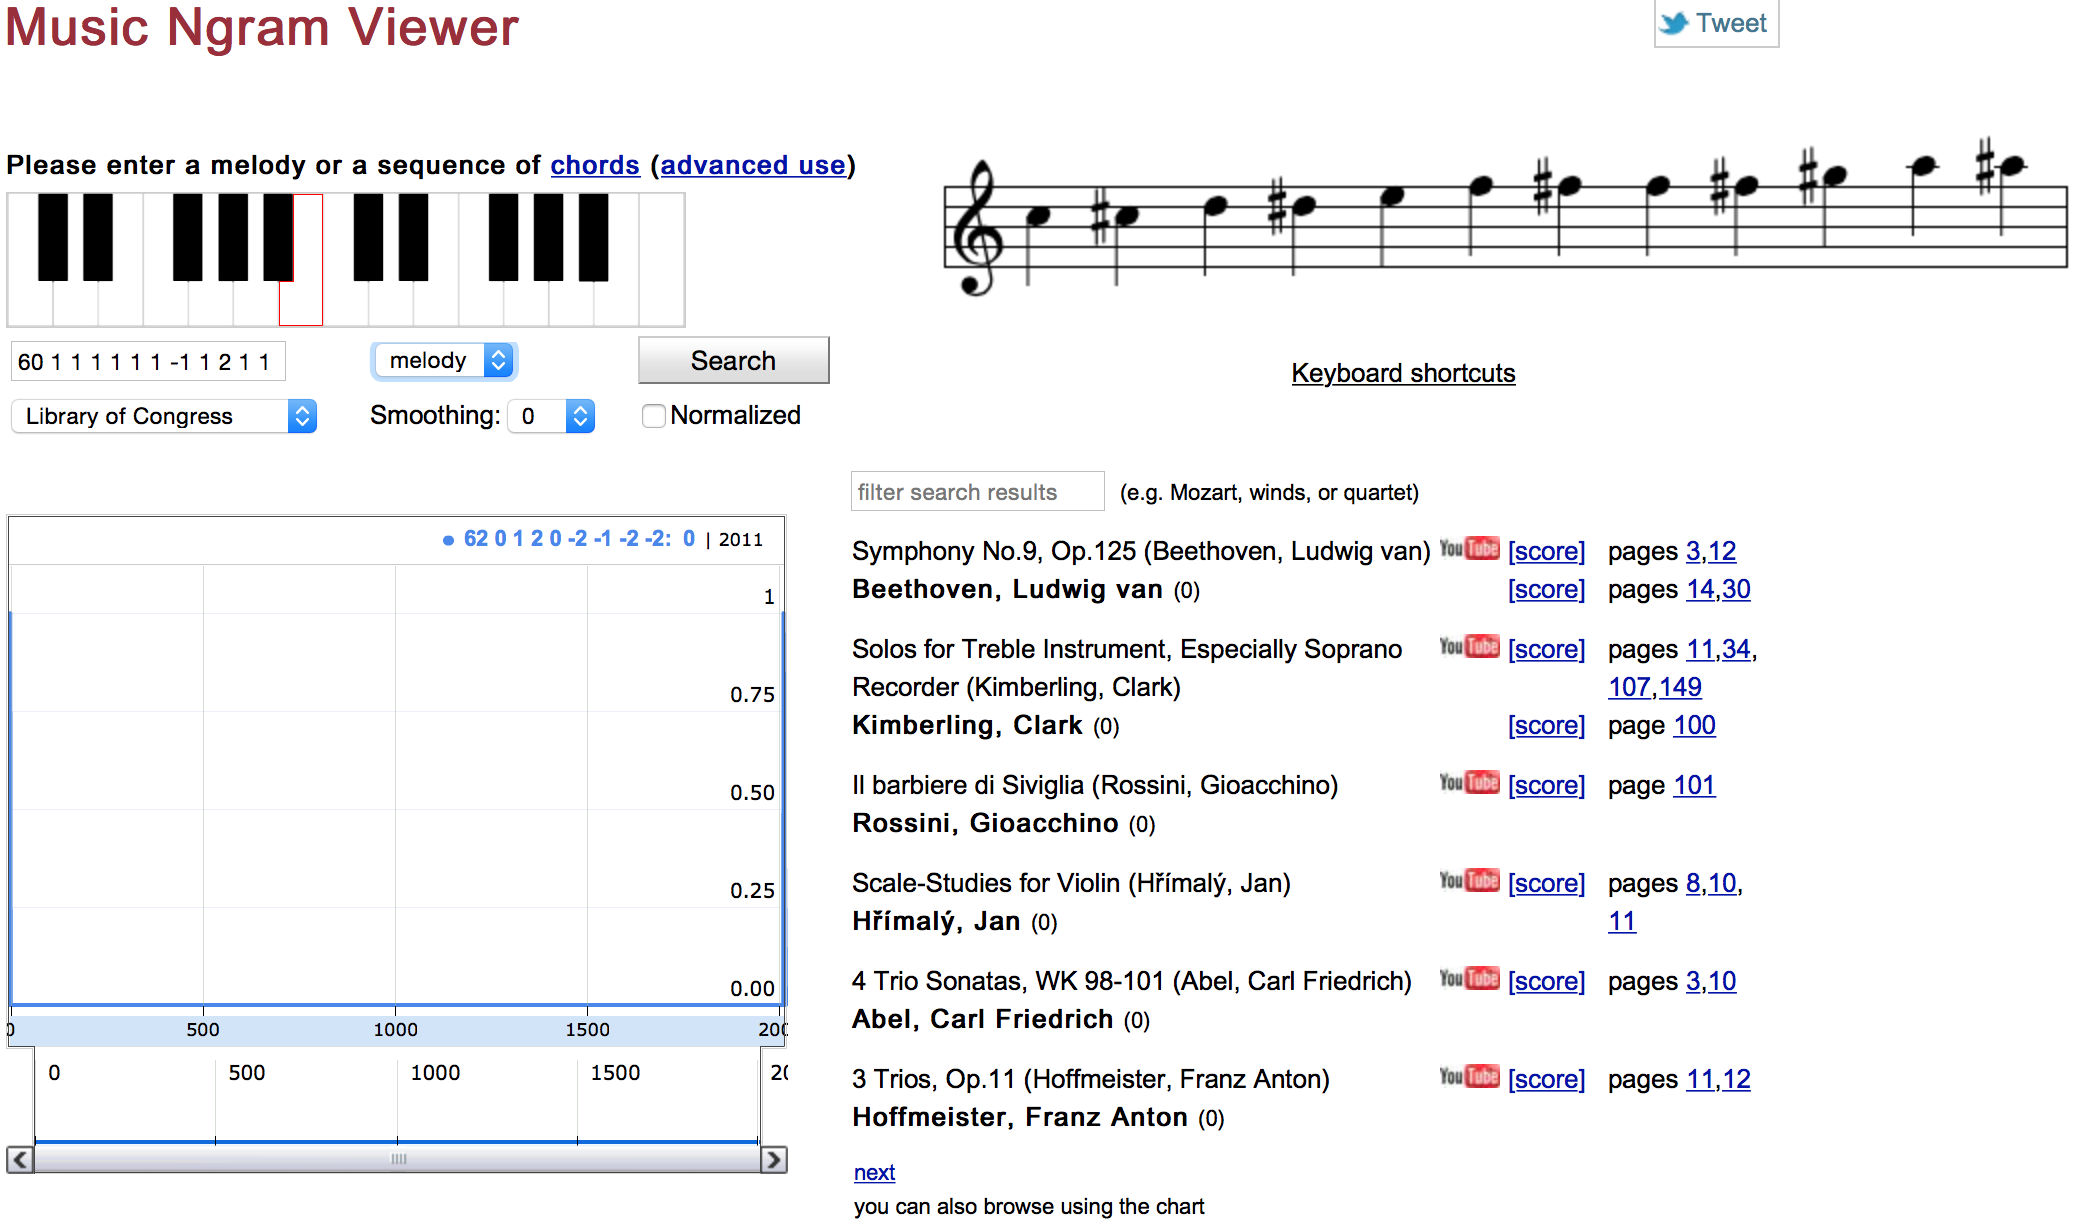
\includegraphics[width=\textwidth]{peachnote}
\caption{Peachnote Ngram Viewer}
\label{fig:peachnote}	
\end{figure}
\floatstyle{plain}
\restylefloat{figure}

Using something similar to the Peachnote interface would make the application more musician-friendly, and would mean that novice musicians would not need to know all of the symbol names in order to query the database.


\subsubsection{Advanced rendering and sound output options}
It is hoped that the project may be expanded so that users can pick and choose what parts and notation are rendered and outputted to sound. 

This would enable the system to be used as a teaching tool, whereby teachers and students could choose to simplify the music by displaying only the symbols they have learned. It would also allow the sound output generator to be used to create accompaniment parts for practice purposes.

\subsubsection{Implementation of paid or subscription APIs}
A further extension of the online API implementation which would be useful is the implementation of new sources which are not open or free. 

This would be useful as these sources, such as MusicNotes which implements a pay-per-piece business model, generally contain a larger variety of sheet music, and at a higher quality as they are generally published by the original arranger or composer.

\subsubsection{Centralisation of APIs}
The current project does all processing of online APIs locally. This could be improved by using a centralised API server, which would communicate with other APIs to access information and scan new files for meta data, which would be stored in a database.

The project would then connect to this API alone, sending formatted query input from the application and receiving suggestions and downloads from the APIs.

This would mean the local user's machine would not have to process XML files which may or may not be requested by the user, and that inclusion of new APIs in the eco system would not require users to update. 

\subsubsection{Online Sharing}
The metadata system currently stores all data to a single SQLite database. This could be expanded in future to offer users the opportunity to upload that data to a centralised online database, in a similar way to the suggested improvement in section 5.3.5.

Users would then be able to browse a larger collection of music from a centralised online point, and request downloads from user created collections. Users who shared their collections would be able to view, accept and reject requests, with an accept resulting in the application uploading the file to the server, sending it to the user requesting the file, and finally, delete the copy on the server.

This functionality would allow users to send files to each other in a more intuitive way than using email or other cloud based services, and wouldn't require much more code or changes to the current system architecture. This may, however, incur problems with licensing which would need to be addressed.

\section{Conclusion}
This project intended to solve the problem of organising sheet music. Sheet music is a visual representation of a piece of music which is given to performers in order to understand how a piece of music is to be performed. The organisation problem has many facets to how it could and should be solved, as some useful information about a piece of music is symbolic and some is bibliographic, some information is general, and some information is specific to each instrument. Automating this process is a feature that previous systems have avoided because the information can be subjective and specific to the context in which the information is needed.

The objectives of having a method to view, organise and expand the collection of music were all met as explained in the evaluation, and therefore this project is considered to be a success. Having an automated information extraction mechanism removes a layer of manual entry when digitising music collections, which should help to move the classical music performance industry into the 21st century. 

Whilst the goals of this project were met, the developer learned that the process of rendering sheet music is a longer process than first expected. The degree of complexity of sheet music notation means that the project does not cover every symbol possible in music composition, but covers enough of the most commonly used symbols to be considered a success.

In the future, it is hoped that more will be done on this project to improve the process of digitising music collections. In particular, conversion from images to the format used in this project would make the process from scanning physical copies of sheet music to organising the collection completely automated. There is further work to be done in improving the rendering capabilities, completing the other secondary objectives and producing an application which works on all platforms, but optical music recognition would be the feature of most use to musicians using this application.


The contributions of this project to the field of music information retrieval and organisation are three fold. The first is a rendering system which could be extended and modified depending on new file input and output as decided by future developers, but which is designed to work well with the input and output sources which are currently integrated. The second is a metadata model which is general enough to cover a wide variety of musicians, but with enough symbolic information that it is of more use than the bibliographic and textual data that other systems provide. The third is the project application itself, which provides a usable, extendable application which could integrate new research on a platform which is designed for musicians, not researchers. The platform could be considered a uniting piece which joins the software development community with the music community.

\begin{appendices}
\section{Mind map of elements of Music}
\section{Initial class diagram}
\section{Revised computerised class diagram}
\section{Initial User Interface Design}
\section{User Interface Feedback survey}
\section{Revised User Interface Design}
\end{appendices}
\section{References}
\printbibliography[heading=none]

\end{document}
